%% History:
% Ondrej Guth (01.05.2015)
% Josef Hlavac & Tomas Zahradnicky (4.10.2010)
%  + Built on the FEL CVUT template by Daniel Sykora and Pavel Tvrdik
%  + Made for FIT CVUT
%  + Joined several chapters and cleaned
%  + Undefined references are typeset in an orange box to alert the writer!
%  + Index is automatically printed if the \usepackage{index} and
%    \newindex{default}{idx}{ind}{Index} lines are uncommented.
%
\documentclass[12pt,oneside,a4paper,final]{memoir}%two-page printing

\usepackage{a4wide}

%\usepackage[T1]{fontenc}


\usepackage[czech]{babel}
\usepackage[utf8]{inputenc} 
\usepackage{lmodern} 
\usepackage[T1]{fontenc}
\usepackage[unicode]{hyperref}
\usepackage{epigraph}
\usepackage{graphicx}
\usepackage{pdflscape}
\usepackage{xfrac}
\usepackage{subcaption}
\usepackage{comment}
\usepackage{tabu}
%\usepackage{svg}
%\usepackage{amsmath}
%\usepackage{setspace}
%\usepackage{epic} % Images drawn in Xfig, exported as .epic

\usepackage{tikz}
\usetikzlibrary{trees}

\usepackage{pdfpages}
\usepackage{colortbl}
\usepackage{xcolor}
\usepackage{array}
\newcolumntype{L}[1]{>{\raggedright\let\newline\\\arraybackslash\hspace{0pt}}m{#1}}
\newcolumntype{C}[1]{>{\centering\let\newline\\\arraybackslash\hspace{0pt}}m{#1}}
\newcolumntype{R}[1]{>{\raggedleft\let\newline\\\arraybackslash\hspace{0pt}}m{#1}}

\usepackage{hyperref}
%\usepackage[hidelinks]{hyperref} %hyperlinks without colour boxes
% \usepackage[usenames]{color}
\usepackage{amssymb}
\usepackage{xspace}
\usepackage{amsmath}
\usepackage{relsize}
\usepackage{amsthm}
\usepackage{listings}
\usepackage{inconsolata}
\usepackage{color} %red, green, blue, yellow, cyan, magenta, black, white
\definecolor{mygreen}{RGB}{28,172,0} % color values Red, Green, Blue
\definecolor{mylilas}{RGB}{170,55,241}

\lstset{language=Matlab,%
    %basicstyle=\color{red},
    basicstyle=\tiny\ttfamily,
    breaklines=true,%
    morekeywords={matlab2tikz},
    keywordstyle=\color{blue},%
    morekeywords=[2]{1}, keywordstyle=[2]{\color{black}},
    identifierstyle=\color{black},%
    stringstyle=\color{mylilas},
    commentstyle=\color{mygreen},%
    showstringspaces=false,%without this there will be a symbol in the places where there is a space
    numbers=left,%
    numberstyle={\tiny \color{black}},% size of the numbers
    numbersep=9pt, % this defines how far the numbers are from the text
    emph=[1]{for,end,break},emphstyle=[1]\color{red}, %some words to emphasise
    %emph=[2]{word1,word2}, emphstyle=[2]{style},    
}



% \usepackage{tikz}
\usepackage[chapter]{algorithm}
% \usepackage{algpseudocode}
% \renewcommand{\algorithmicrequire}{\textbf{Input:}}
% \renewcommand{\algorithmicensure}{\textbf{Output:}}

%\usepackage{proof}
%\usepackage{latexsym}
% \usepackage{rotating}
%\usepackage{epsfig}
% \usepackage{subfigure}
% \usepackage{multirow}
%\usepackage{index}
%\newindex{default}{idx}{ind}{Index}

\usepackage[
nonumberlist, %do not show page numbers
acronym,      %generate acronym listing   -> Not used in this example (see line with %%% )
nomain,
numberedsection
% notoc,          %show listings as entries in table of contents
]      %use section level for toc entries
{glossaries}
%\makeglossaries
\input tex/phdmacro.tex %couple of macros for formatting the dissertation thesis,
                    %your personal and specific macros can be placed also there


\renewcommand{\labelitemi}{\(\circ\)}

\newenvironment{chapterintro}{\slshape}{\par}

\usepackage{etoolbox}
% fix TOC in memoir class
\makeatletter
\renewcommand{\@pnumwidth}{2em} 
\renewcommand{\@tocrmarg}{3em}
\patchcmd{\@endtheorem}{\@endpefalse}{}{}{}
\patchcmd{\endproof}{\@endpefalse}{}{}{}
\makeatother

\newcommand\DissTitle{Hodnocení kvality zvuku v systémech digitálního rozhlasového vysílání\\\small \medskip Audio Quality Assessment of Digital Radio Broadcasting Systems}
\newcommand\FirstandFamilyName{Adam Bartyzal}
\newcommand\Email{bartyada@fel.cvut.cz}
\newcommand\Month{Praha, Květen}
\newcommand\Year{2019}
\newcommand\Supervisor{Ing. Karel Ulovec, Ph.D.}
\newcommand\SupervisorAffiliation{
Katedra radioelektroniky\\
%Department of Digital Design\\
%Department of Software Engineering\\
% Department of Computer Systems\\
Fakulta elektrotechnická\\
České Učení Vysoké Technické v Praze\\
Technická 2\\
160 00 Praha 6\\
Česká Republika}
%%-> uncomment if you have a thesis co-supervisor
%\newcommand\CoSupervisor{prof. RNDr. COSUPERVISOR, Ph.D.}
%\newcommand\CoSupervisorAffiliation{
%Computer Science and Engineering Department\\
%Faculty of Electrical Engineering\\
%Czech Technical University in Praha\\
%Karlovo n\'{a}m.~13\\
%121 35 Praha 2\\
%Czech Republic}

\newcommand\PhDProgram{Rádiová a optická technika}
%\newcommand\PhDSpecialization{Informatics}
\newcommand\Department{Katedra elektromagnetického pole}
%\newcommand\Department{Department of Digital Design}
%\newcommand\Department{Department of Software Engineering}
% \newcommand\Department{Department of Computer Systems}
\newcommand\Faculty{Fakulta elektrotechnická}
\newcommand\University{České Učení Vysoké Technické v Praze}
\newcommand\Address{Technická 2, 160 00 Praha 6, Česká Republika}

\def\UrlBreaks{\do\/\do\-}



\newacronym{DFA}{DFA}{deterministic finite automaton}
\newacronym{NFA}{NFA}{nondeterministic finite automaton}
\newacronym{FA}{FA}{finite automaton}

\maxsecnumdepth{subsubsection}
\setcounter{tocdepth}{2}
\makeheadstyles{FITthesis}{
	\chapterstyle{madsen}
	\setsecheadstyle{\Large\bfseries\sffamily}
	\setsubsecheadstyle{\large\bfseries\sffamily}
	\setsubsubsecheadstyle{\bfseries\sffamily}
}
\headstyles{FITthesis}

% \includeonly{
% 	tex/abstract
% 	,tex/acknowledgement
% 	,tex/introduction
% 	,tex/stateoftheart
% 	,tex/conclusions
% }

\begin{document}
\tikzstyle{every node}=[draw=black,thick,anchor=west]
\theoremstyle{definition}
\newtheorem{lemma}{Lemma}[section]
\newtheorem{theorem}[lemma]{Theorem}
\newtheorem{definition}[lemma]{Definition}
\newtheorem{preposition}[lemma]{Preposition}
\newtheorem{example}[lemma]{Example}
\newtheorem{corollary}[lemma]{Corollary}
\newtheorem{proposition}[lemma]{Proposition}
\newtheorem{property}[lemma]{Property}
\newtheorem{observation}[lemma]{Observation}
\theoremstyle{remark}
\newtheorem{notation}[lemma]{Notation}
\newtheorem{note}[lemma]{Note}

\setlength\epigraphwidth{1\textwidth}
\setlength\epigraphrule{0pt}

% allow @ to appear in macro names
% \makeatletter

% % produce undefined references in an orange box rather than just ??
% \def\@setref#1#2#3{%
%   \ifx#1\relax
%    \protect\G@refundefinedtrue
%    \nfss@text{\reset@font\bfseries\fcolorbox{black}{Orange}{??}}%
%    \@latex@warning{Reference `#3' on page \thepage \space
%              undefined}%
%   \else
%    \expandafter#2#1\null
%   \fi}


\frontmatter

\coverpagestarts

\pagestyle{ruled}

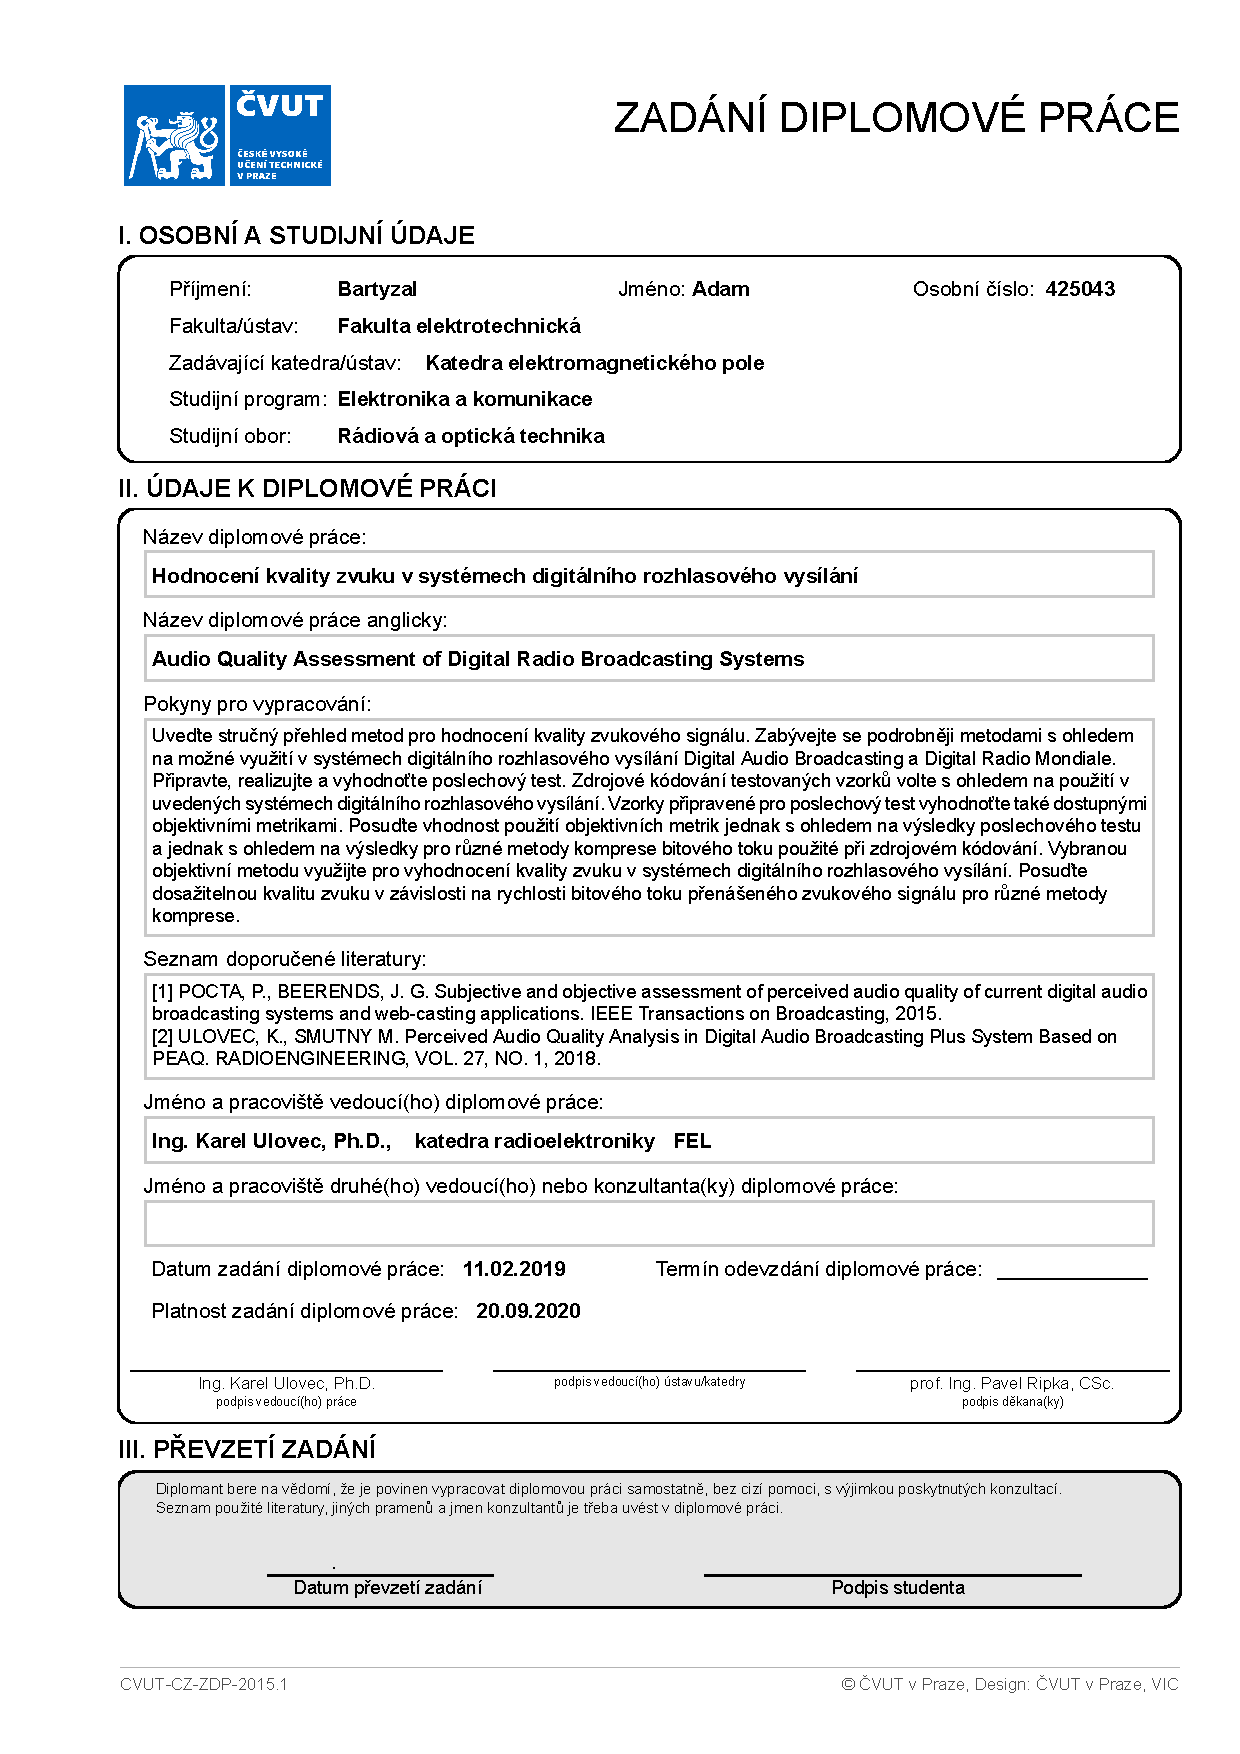
\includepdf[pages={1}]{pdf/zav_prace.pdf}

\chapter*{Prohlášení}
\label{declaration}



Prohlašuji, že jsem předloženou práci vypracoval samostatně a že jsem uvedl veškeré použité informační zdroje v souladu s Metodickým pokynem o dodržování etických principů při přípravě vysokoškolských závěrečných prací.

\vfill


\noindent V Praze dne....................................... \hfill .......................................Podpis Autora




\chapter*{Poděkování}
\label{chap:acknowledgement}

Rád bych tímto poděkoval Ing. Karlu Ulovcovi, Ph.D. a Ing. Františku Rundovi, Ph.D. za cenné rady a konzultace týkající se akademické stránky diplomové práce. Dále bych chtěl vyjádřit dík členům mé rodiny a mým přátelům za podporu psychickou, která byla snad ještě důležitější.

\vfill

\null\hfill Tato práce byla podpořena grantem studentské grantové soutěže \\ \null\hfill ČVUT č. SGS17/190/OHK3/3T/13





\chapter*{Abstrakt}
\label{abstract:czech}

Diplomová práce se věnuje problematice hodnocení kvality zvuku ve vztahu k nastavení parametrů vysílání v systémech digitálního rádia. Nejprve jsou stručně popsány systémy DAB/DAB+, DRM(+) a techniky zdrojového kódování zvuku. Další část se věnuje postupům hodnocení poslechové kvality. Napřed je uveden přehled subjektivních poslechových metod a poté jsou vysvětleny principy objektivního testování různými počítačovými algoritmy. Praktická část se soustředí na realizaci poslechových testů MUSHRA a objektivního testování užitím čtyř různých metrik: PEAQ Basic, PEAQ Advanced, PEMO-Q a ViSQOL. Pomocí výsledků subjektivního testování je určena nejlepší metoda, která je následně použita k vyhodnocení kvality přenášeného zvukového signálu v závislosti na bitovém toku a způsobu komprese.

\bigskip

\noindent\textbf{Keywords:}

~digitální rádio, hodnocení kvality zvuku, MUSHRA, PEAQ, PEMO-Q, ViSQOL.

\vfill


\chapter*{Abstract}
\label{abstract:english}

The thesis deals with the issue of sound quality evaluation in relation to the setting of broadcasting parameters in digital radio systems. In the beginning, DAB/DAB+, DRM(+) systems and audio source coding techniques are briefly described. The next part focuses on the procedures of listening quality assessment. First, an overview of subjective listening methods is given, and then the principles of objective testing by various computer algorithms are explained. The practical part focuses on the implementation of listening MUSHRA tests and objective testing using four different metrics: PEAQ Basic, PEAQ Advanced, PEMO-Q and ViSQOL. Using subjective testing results the best method is chosen and used to evaluate the quality of the transmitted audio signal, depending on bitrate and compression method.

\bigskip

\noindent\textbf{Keywords:}

~digital radio, sound quality assessment, MUSHRA, PEAQ, PEMO-Q, ViSQOL.

\vfill


% \newpage
%\chapter*{Poděkování}
\label{chap:acknowledgement}

Rád bych tímto poděkoval Ing. Karlu Ulovcovi, Ph.D. a Ing. Františku Rundovi, Ph.D. za cenné rady a konzultace týkající se akademické stránky diplomové práce. Dále bych chtěl vyjádřit dík členům mé rodiny a mým přátelům za podporu psychickou, která byla snad ještě důležitější.

\vfill

\null\hfill Tato práce byla podpořena grantem studentské grantové soutěže \\ \null\hfill ČVUT č. SGS17/190/OHK3/3T/13





% \newpage
%\include{tex/dedication}
% \newpage

\tableofcontents*
%------------------------------
%  LOF, LOT
%----------------------------------------------------------------------------------------------------------
% \newpage\addcontentsline{toc}{chapter}{\protect\numberline{}{List of Figures}}

\clearpage
\listoffigures*
% \newpage\addcontentsline{toc}{chapter}{\protect\numberline{}{List of Tables}}

\clearpage
\listoftables*
% \newpage\addcontentsline{toc}{chapter}{\protect\numberline{}{List of Algorithms}}

%\clearpage
%\listofalgorithms

% \newpage\addcontentsline{toc}{chapter}{\protect\numberline{}{Definitions, Notations and Abbreviations}}\input{tex/definitions.tex}
%----------------------------------------------------------------------------------------------------------
% \newpage
\setsecnumdepth{part}
%\chapter*{Seznam symbolů a zkratek}

\textbf{Použité symboly}

\begin{tabular}{ll}
{$\mathbb N$} & Natural numbers set

\end{tabular}
\vskip 1cm

\noindent\textbf{Použité zkratky}

\begin{tabular}{ll}
ITU & Mezinárodní telekomunikační unie\\
SDG & \textit{Subjective difference grade}\\
ODG & \textit{Objective difference grade}\\
GUI & Grafické uživatelské rozhraní\\
STFT & \textit{Short Time Fourier Transform}\\
MPEG & Motion Picture Experts Group\\



\end{tabular}




% \mainbodystarts
\mainmatter

%\singlespacing
%\onehalfspacing
%\doublespacing
%\part{The Parameter Extraction Methodology}
%-----------------------
%  Chapters start here
\chapter{Úvod}
\label{chap:introduction}

\epigraph{\hfill\textit{Zkuste to bez drátů, milý Marconi!}}{-Ladislav Smoljak, Zdeněk Svěrák, \textit{Jára Cimrman ležící, spící}}

%\section{Letmý pohled do historie vysílání}
Letmým pohledem do historie můžeme zjistit, že rozhlasové vysílání je tu s námi už zhruba jedno století. V roce 1922 bylo v Anglii zahájeno první pravidelné rozhlasové vysílání BBC (\textit{British Broadcasting Corporation}). Jen rok na to následoval počátek vysílání i na území Československa. Tehdejší Český rozhlas Radiojournal vysílal monofonně amplitudovou modulací a ta přenášela převážně mluvené slovo skrz éter až do roku 1959, kdy se k ní připojila modulace frekvenční.\cite{web:cro} Postupem času se k rádiím připojily i další technologie jako například televizní vysílání, telekomunikační či datové služby a elektromagnetické spektrum začalo být velmi ceněnou komoditou.

%\section{Důvody k digitalizaci}
Snaha o rozšíření nabízeného obsahu a zároveň o minimalizaci využitého pásma vedla k myšlence digitalizace rozhlasového vysílání. Digitální rádio, přenášející zvuk ve formě jedniček a nul, umožnilo využít kompresních algoritmů a tím výrazně snížit spektrální náročnost. Tento krok ovšem postavil před poskytovatele vysílání nelehký úkol. Jaké parametry přenosu nastavit, aby posluchač nepostřehl vliv digitální komprese. Jinými slovy jak zachovat dostatečnou kvalitu zdrojového signálu a zároveň docílit co nejefektivnějšího přenosu. Řešení tohoto problému se nalézalo ve výsledcích poslechových testů. Aby byly výsledky testů relevantní, bylo třeba zaručit různorodost vzorků, dostatečné množství subjektů a správnou metodiku. Staré rčení ovšem říká \uv{Čas jsou peníze} a nejinak tomu je i v případě subjektivních testů. 


Rozvoj výpočetní techniky ovšem umožnil nahradit skupiny lidí v poslechových místnostech algoritmy, odhadujícími kvalitu zvuku zakódovaného ztrátovou kompresí. Ta na rozdíl od komprese bezztrátové, nesnižuje pouze entropii dat, nýbrž z původního zdroje odstraňuje irelevanci. Jaká data mohou být označena za irelevantní pro poslech lidským uchem zkoumá ve světe zvukového zpracování obor zvaný psychoakustika. Kodeky využívají objevů této vědní disciplíny, jimiž jsou například spektrální či časové maskování, ve prospěch úspory dat. Obecně se dá říci, že čím modernější kodek je, tím více těchto poznatků využívá. To je sice velice pozitivní z hlediska přenosu signálů skrze kanál, nicméně se ukazuje, že algoritmy určené pro objektivní hodnocení audiosignálů si s takovýmto vývojem neumí dobře poradit a výsledky hodnocení dopadají při použití nových efektivnějších kodeků hůře, než kdyby byl hodnotícím prvkem lidský posluchač. To ve výsledku může vést k nesprávnému nastavení parametrů přenosu v digitálním rádiu a tím k neefektivnímu využití spektra. 

Ověřením zda k tomuto jevu dochází a v jaké míře se zabývá tato diplomová práce. V následujících kapitolách je uveden vhled do systémů digitálních rádií a v nich používaného zdrojového kódování. Dále je zde přiblížena problematika subjektivního a objektivního hodnocení audiosignálů. Podrobně jsou popsány jednotlivé metody, jenž jsou poté v praktické části využité k testování zvukových vzorků zpracovaných různými kompresními metodami. Dále je v práci popsáno, jaké programové vybavení bylo vyvinuto a využito a v závěru se práce věnuje výsledkům jednotlivých testů společně s jejich souvislostmi. Na jejich základě je vybrána a použita nejvhodnější metoda k vyhodnocování kvality zvuku v systémech digitálního rozhlasu.

\chapter{Digitální rádio a metody komprese audiosignálu}
\label{chap.digitalRadio}

\epigraph{\textit{\hfill Video killed the radio star.}}{The Buggles, \textit{název písně}}

Přestože smrt rádia prorokovali \uv{The Buggles} v historicky prvním videoklipu vysílaném hudební televizí MTV (\textit{Music Television}), analogové rádio je tu s námi dodnes a v následujících letech pravděpodobně bude i nadále. Zdá se že minimálně do roku 2025, dokdy v České Republice platí licence na pásma, ve kterých je klasické FM rádio provozováno. Nicméně digitalizace je všudypřítomný trend a podobně jako se v průběhu poslední dekády přecházelo na digitální vysílání televize DVB-T (\textit{Digital Video Broadcasting – Terrestrial}), čeká nás modernizace i ve vysílání rozhlasových služeb. 

\section{Standardy digitálního rozhlasového vysílání}

V současné době existují dva velké paralelně existující standardy. DAB (\textit{Digital Audio Broadcasting}), ke kterému se po úspěchu v severských zemích upínají i tuzemští poskytovatelé rozhlasových služeb, a DRM (\textit{Digital Radio Mondiale}), momentálně zažívající \uv{boom} v Indii a dalších zemích, kde je rádio provozováno v pásmu středně dlouhých vln. Vedle nich existují i další systémy, jako například Japonský ISDB (\textit{Integrated Services Digital Broadcasting}) standard pro vysílání televize a rádia, nahrazující tamější analogový NTSC-J (\textit{National Television System Committee - Japan}), či IBOC (\textit{In-band on-channel}) užívaný v Americe pod obchodním názvem HD Radio, který vysílá analogový a digitální signál simultánně. Tyto druhy vysílání se ovšem nevztahují k evropské půdě a tudíž se práce v následujících dvou podkapitolách zabývá pouze systémy DAB/DAB+ a DRM(+).

\subsection{Digital Audio Broadcasting}

Standard \textit{EUREKA 147 Digital Audio Broadcasting} (zkráceně DAB) popsaný v normě ETSI EN 300 401\cite{etsi:dab} je normou vyvíjenou již od osmdesátých let Evropským ústavem pro telekomunikační normy ETSI (\textit{European Telecommunications Standards Institute}) společně s Mezinárodní telekomunikační unií ITU (\textit{International Telecommunication Union}). Jedná se o moderní a univerzální multimediální rozhlasový systém, jehož cílem je nahradit současné FM vysílání. Oproti tomu se pyšní například odolností vůči aditivnímu šumu, kvalitou zvuku srovnatelnou se záznamem na CD, energetickou úsporností a možností využití ve více pásmech. Balík několika rozhlasových stanic společně s doprovodnými datovými službami multiplexuje do jednoho datového toku, který je poté vysílán modulací OFDM (\textit{Orthogonal frequency-division multiplexing}), jejíž hlavní předností je odolnost vůči chybám způsobeným vícecestným šířením a možnost využití jedno-frekvenční sítě.

%\subsection{Vysílací módy}

Starší verze systému DAB \cite{etsi:dab:old}, byla navržena pro přenos různými technologiemi v několika pásmech jak je ukázáno v tabulce \ref{table:dab}. Definovány byly 4 vysílací módy, které umožňovaly vysílání až do frekvencí kolem 3 GHz. Ve verzi 2.2.1 doporučení ETSI EN 300 401 \cite{etsi:dab} z ledna 2017 se už s módy II - IV nadále nepočítá a DAB+ tak zůstává ryze terestrickou platformou.

\begin{table}[ht]
\centering
\begin{tabular}{|c|c|c|c|c|}
\hline
\textit{\textbf{}} & \textbf{Mód I} & \textbf{Mód II} & \textbf{Mód III} & \textbf{Mód IV} \\ \hline
Použití & \begin{tabular}[c]{@{}c@{}}Pozemní \\ VHF\\  168 - 240 MHz\end{tabular} & \begin{tabular}[c]{@{}c@{}}Pozemní \\ L pásmo\\  1452 - 1492 MHz\end{tabular} & \begin{tabular}[c]{@{}c@{}}Satelitní \\ L pásmo\\ až do 3 GHz\end{tabular} & \begin{tabular}[c]{@{}c@{}}Městská \\ zástavba\\  L pásmo\end{tabular} \\ \hline
\begin{tabular}[c]{@{}c@{}}Počet nosných vln\\ frekvencí\end{tabular} & 1536 & 384 & 192 & 768 \\ \hline
\begin{tabular}[c]{@{}c@{}}Odstup nosných vln\\ {[}kHz{]}\end{tabular} & 1 & 4 & 8 & 2 \\ \hline
\begin{tabular}[c]{@{}c@{}}Trvání intervalu \\ {[}$\mu$s{]}\end{tabular} & 1246 & 311,5 & 155,75 & 623 \\ \hline
\begin{tabular}[c]{@{}c@{}}Délka ochranného\\ intervalu\end{tabular} & 246,0 & 61,5 & 30,75 & 123 \\ \hline
\end{tabular}
\caption{Provozní módy DAB/DAB+ \cite{etsi:dab}}
\label{table:dab}
\end{table}

%\subsection{Principy}

Norma \cite{etsi:dab} definuje pouze vznik signálu na vysílací straně. Řešení na přijímací straně je ponecháno na výrobci koncových zařízení. Na obrázku \ref{pic:dab} je ukázáno jak je sestavení DAB signálu řešeno.

\begin{figure}[h]
    \centering
    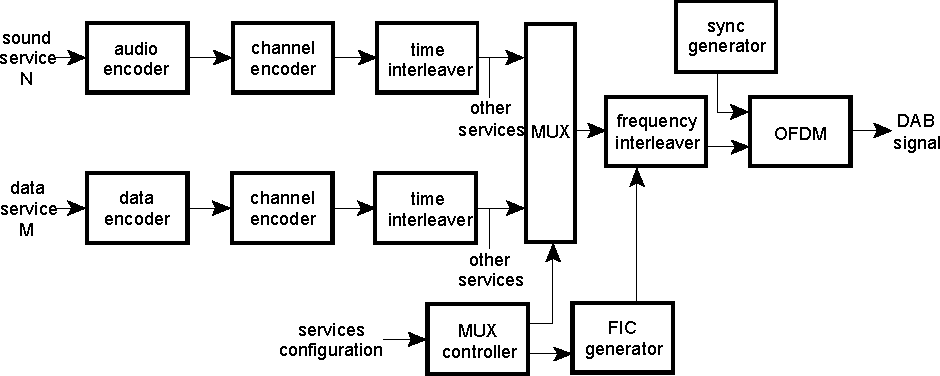
\includegraphics[width=.9\textwidth]{pic/dab.pdf}
    \caption{Blokové schéma sestavení DAB/DAB+ signálu.\cite{etsi:dab}}
    \label{pic:dab}
\end{figure}

Z hlediska zdrojového kódování využívá původní DAB kodek MPEG-1 Audio Layer II (více o kodecích v podkapitole \ref{subchap:codecs}). Je možno použít dva vzorkovací kmitočty: 24 kHz a 48 kHz. Od těch se odvíjí možné bitové rychlosti zdrojového kódování vypsané v tabulkách \ref{table:dabbitrates1} a \ref{table:dabbitrates2}. Výstupem kodéru jsou logické rámce (\textit{Logical Frames}) trvající 48 ms respektive 24 ms pro vyšší vzorkovací rychlost.
V novější verzi DAB+ metodu MPEG Layer II doplnil modernější  kódovací postup HE-AAC v2. Tok nového kodéru je opatřen Reed-Solomonovým ochranným kódem a je vkládán do superrámců (\textit{Super Frames}), dlouhých 120 ms, které jsou rozděleny do pěti logických rámců DAB. Počet vzorkovacích kmitočtů vyrostl na čtyři. Konkrétně: 16, 24, 32, 48 kHz a možné bitové rychlosti jsou násobky osmi od 8 kb/s až do 192 kb/s.

\begin{table}[h]
\centering
\begin{tabular}{|c|c|c|c|c|c|c|c|c|}
\hline
48 kHz jednokanálový mód (kb/s) & 56 & 64 & 80 & 96 & 112 & 128 & 160 & 192 \\ \hline
48 kHz ostatní módy (kb/s) & 112 & 128 & 160 & 192 & 224 & 256 & 320 & 384 \\ \hline
\end{tabular}
\caption{Dostupné bitové rychlosti při použití MPEG Layer II a vzorkovací rychlosti 48 kHz \cite{etsi:mp2}}
\label{table:dabbitrates1}
\end{table}

\begin{table}[h]
\centering
\begin{tabular}{|c|c|c|c|c|c|c|c|c|c|c|c|c|c|c|}
\hline
24 kHz (kb/s) & 8 & 16 & 24 & 32 & 40 & 48 & 56 & 64 & 80 & 96 & 112 & 128 & 144 & 160 \\ \hline
\end{tabular}
\caption{Dostupné bitové rychlosti při použití MPEG Layer II a vzorkovací rychlosti 24 kHz \cite{etsi:mp2}}
\label{table:dabbitrates2}
\end{table}


Po odstranění irelevantních a nadbytečných dat zdrojovým kodérem, přichází na řadu přidání pečlivě řízené redundantní složky pomocí konvolučního kodéru, který je následován časovým prokladačem. Ten determinovaným způsobem přeskládá tok dat tak, že při zpětném složení se případná shluková chyba, vzniklá při přenosu kanálem, \uv{rozmělní} a může být opravena konvolučním kódem. Maximální možné přenosové rychlosti multiplexu DAB v závislosti na stupni ochrany jsou v tabulce \ref{table:dabcoderates}.

\begin{table}[h]
\centering
\begin{tabular}{|c|c|c|}
\hline
Stupeň ochrany & Kódový poměr & Kapacita multiplexu (kb/s) \\ \hline
1-A & 1/4 & 576 \\ \hline
2-A & 3/8 & 864 \\ \hline
3-A & 1/2 & 1152 \\ \hline
4-A & 3/4 & 1728 \\ \hline
\end{tabular}
\caption{Přehled dostupných přenosových rychlostí v DAB/DAB+ pro dostupné stupně ochrany a kódové poměry}
\label{table:dabcoderates}
\end{table}

Počet programů v multiplexu DABu je flexibilní, zrovna tak jako nastavení kvality jednotlivých zvukových služeb a jejich doprovodných informací.

Ortogonálně frekvenčně dělený multiplex, neboli OFDM je modulace využívající velkého množství nosných vln. Dostupná šířka pásma je rozdělena do ortogonálních subkanálů. Ty jsou od sebe vzdáleny $\Delta f = \frac{1}{T}$, kde $T$ je doba trvání jednoho symbolu. Signál omezený v čase si lze představit jako signál trvající nekonečně dlouho vynásobený obdélníkovým pulzem. Takovému signálu ve frekvenčním spektru odpovídá výkonová hustota popsaná funkcí $\frac{\sin{x}}{x}$. Průchody nulou jednotlivých nosných vln jsou umístěny přesně na sebe, díky čemuž jsou postranní laloky potlačeny, jak naznačuje obrázek \ref{pic:ofdm}.

\begin{figure}[h]
    \centering
    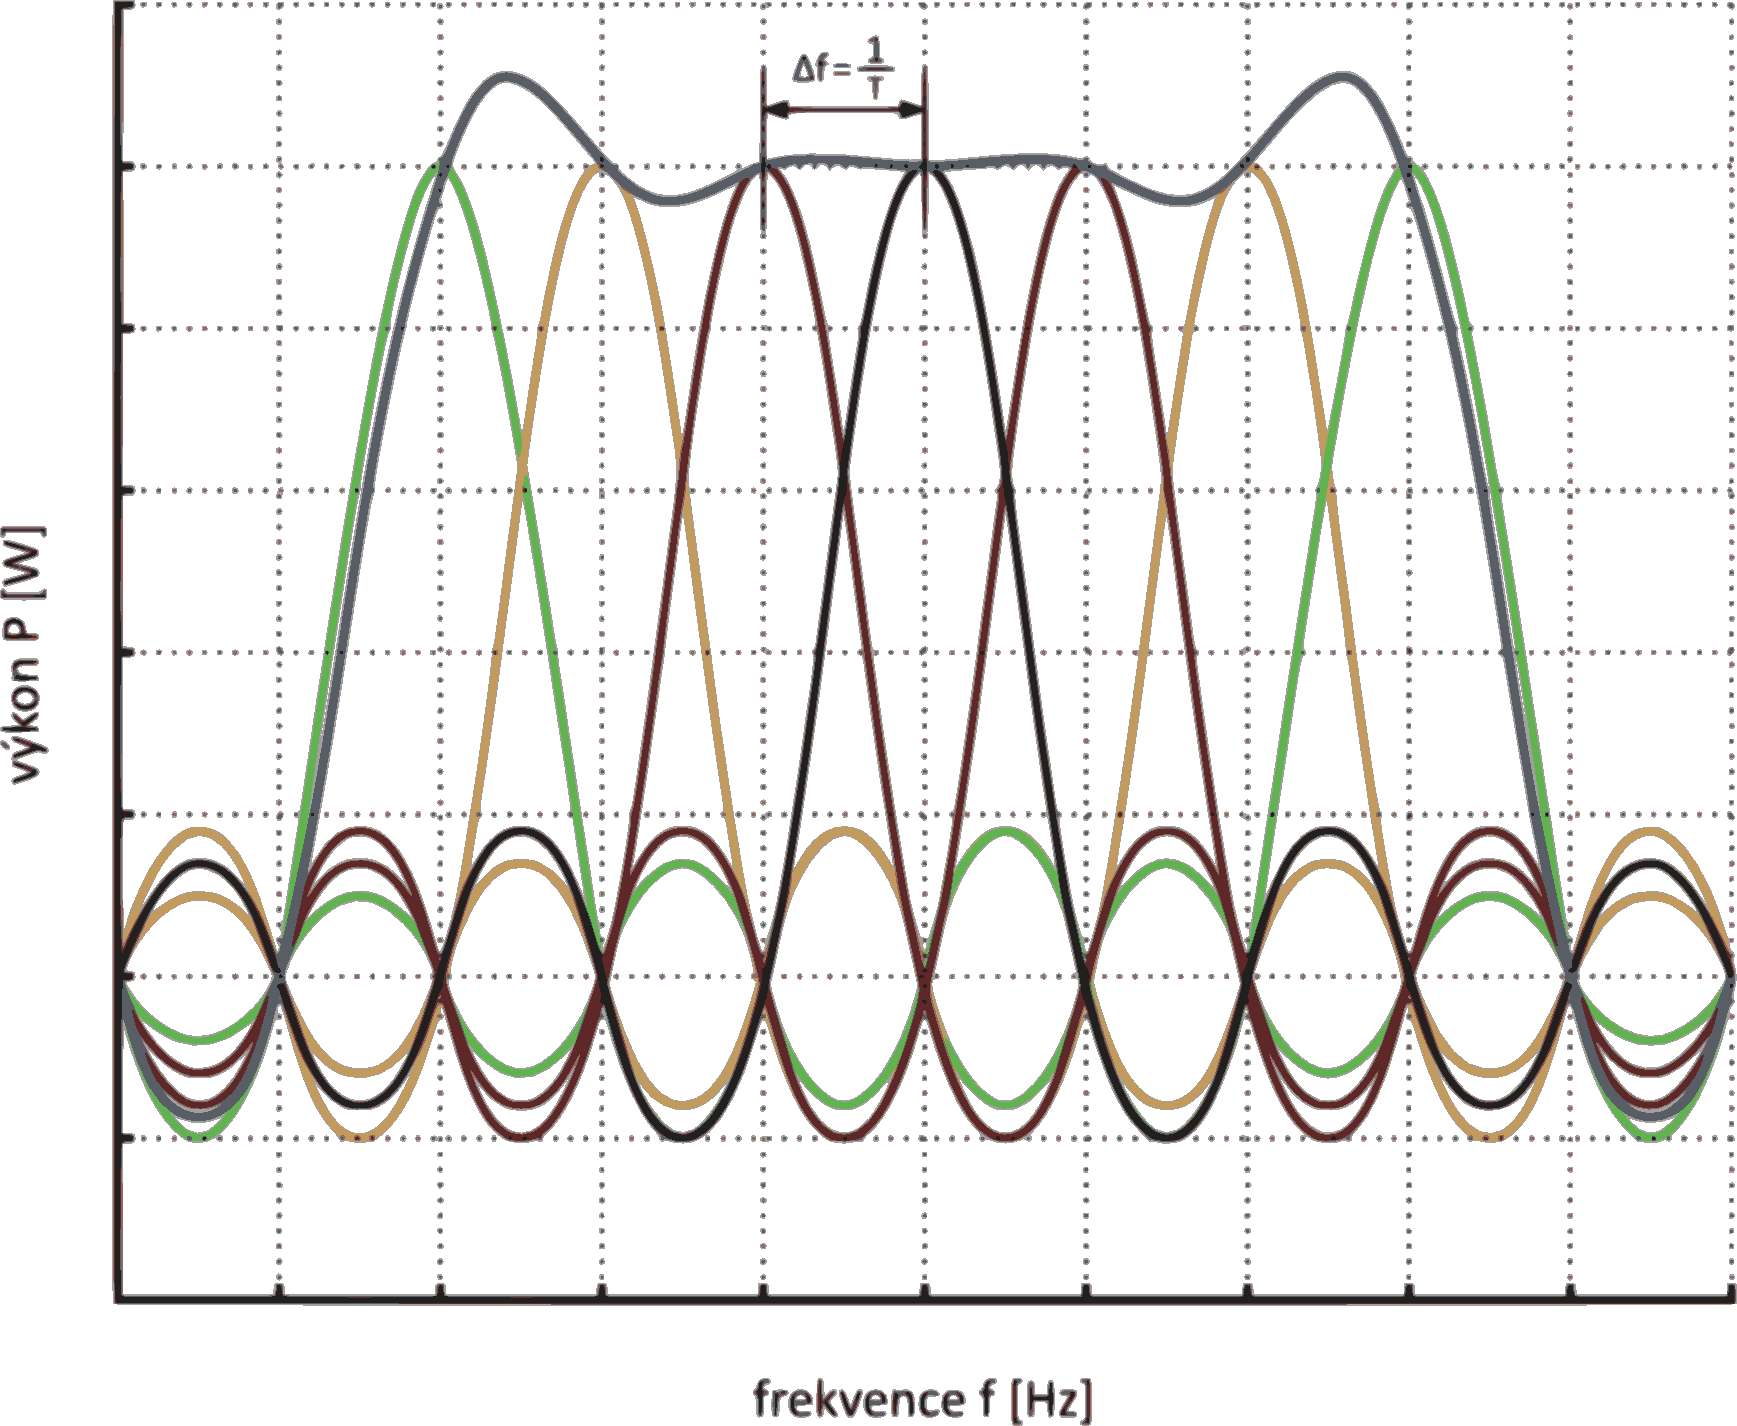
\includegraphics[width = .5\textwidth]{pic/ofdm2.pdf}
    \caption{Naznačení principu rozmístění nosných kmitočtů v systému OFDM \cite{web:ofdm}}
    \label{pic:ofdm}
\end{figure}


K čemu velké množství nosných frekvencí? Zjednodušeně řečeno, čím více nosných vln, tím delší symbolový čas $T$. Odražený signál, který do přijímače dorazí s časovým zpožděním může způsobit chybnou detekci symbolu. Dobře se to dá představit na analogové televizi, kde zpožděný signál způsobil chybu známou jako \uv{duch}. V digitálním světě sice \uv{duchové} neexistují, zato vznikne překryv symbolu zpožděného signálu se symbolem následujícího rámce, tedy jev známý jako mezisymbolová interference ISI (\textit{Inter Symbol Interference}). Prodloužení symbolového času způsobí to, že mírně zpožděný signál dorazí stále \uv{včas} a nedojde k znehodnocení přijatého symbolu. I přesto ve zlomku vysílacího času vzniká překryv dvou symbolů a proto je do vysílání vkládán ochranný interval GI (\textit{Guard Interval}), neboli čas, kdy je vysílání pozastaveno. Tím na jednu stranu klesá efektivita přenosu, nicméně signál je díky tomu značně odolnější vůči odrazům. Zároveň to umožňuje konstruovat sítě s vysílači na téže frekvenci, čímž dochází k značné úspoře spektra.    

Jednotlivé nosné vlny jsou v systému DAB modulovány čtyř stavovým fázovým klíčováním s pamětí neboli DQPSK (Differential Quadrature Phase-Shift Keying).

\subsection{Digital Radio Mondiale (+)}


Na rozdíl od systému DAB, který postupně nahrazuje FM vysílání pouze v pásmu velmi krátkých vln, si DRM brousí zuby i na stanice vysílané amplitudovou modulací ve středních a dlouhých vlnách. ETSI ho definuje normou \textit{ETSI ES 201 980} \cite{etsi:drm}, a k dnešnímu dni existují jeho dvě verze: DRM30 a DRM+. Novější verze standard doplnila o módy pro použití v pásmu VKV a také o modernější druhy zdrojového kódování.

%\subsection{Principy}

Blokové schéma vysílače DRM je znázorněno na obrázku \ref{pic:drm}. V Multiplexu systému DRM je ve srovnání s digitálním rádiem DAB podstatně menší počet rozhlasových stanic. Typicky jedna, maximálně však čtyři (včetně doplňkových dat). To může být výhodou pro poskytovatele obsahu. Odpadá jim tak problematika složitého domlouvání se s konkurencí a tím je mimo jiné zajištěna větší nezávislost. 

\begin{figure}[h]
    \centering
    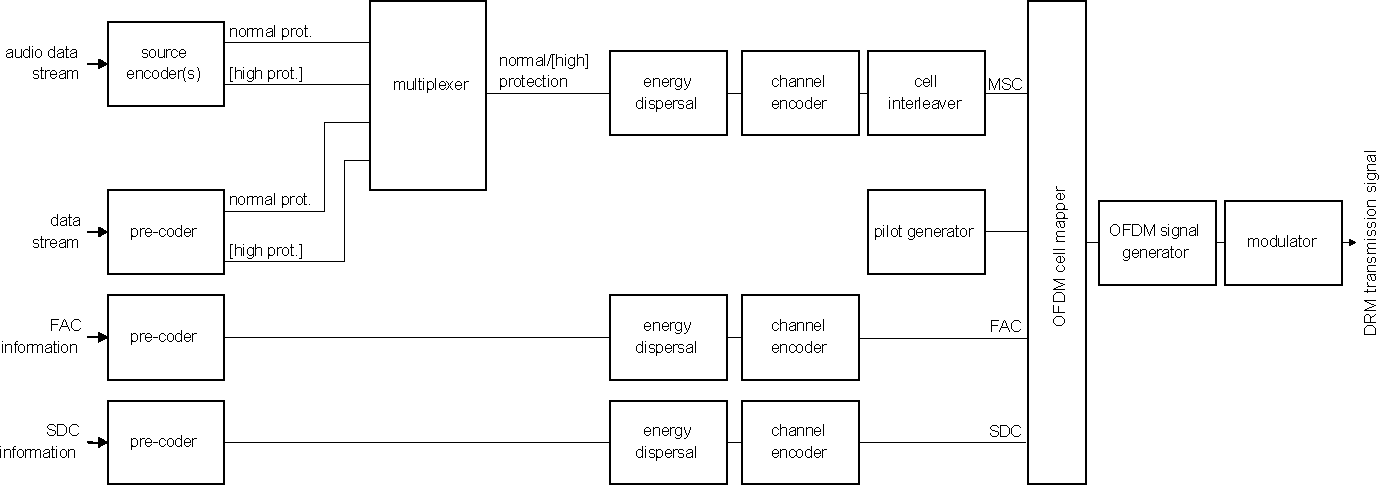
\includegraphics[width=1\textwidth]{pic/drm.pdf}
    \caption{Blokové schéma DRM systému \cite{etsi:drm}}
    \label{pic:drm}
\end{figure}

Pro kanály umístěné ve spektru pod hranicí 30 MHz, nabízí DRM vzhledem k použité modulaci prostor pro datový tok od 8 kb/s po 72 kb/s. Pro kanály nad 30 MHz maximální bitová rychlost povyroste až na 186 kb/s. Nabídka systémů zdrojového kódování je následující:
\begin{itemize}
    \item MPEG-4 CELP, MPEG-4 XVHC - pro monofonní kódování mluveného slova
    \item MPEG-4 HE-AAC v2 - pro kódování hudebních stanic
    \item MPEG xHE-AAC - univerzální kodek pro řeč a hudbu
    \item MPEG Surround - pro kódování doplňkových stop při vícekanálovém přenosu
\end{itemize}

\smallskip

Výsledný datový tok se skládá ze třech kanálů:
\begin{itemize}
    \item MSC (\textit{Main Service Channel}) - kanál obsahující audio a datové služby
    \item FAC (\textit{Fast Acces Channel}) - informace určené k demodulování signálu 
    \item SDC (\textit{Service Description Channel}) - informace potřebné k dekódování MSC
\end{itemize}

Každý z bloků má svůj mírně specifický kanálový kodér. Scrambler zajišťuje pseudonáhodný charakter signálu, čímž vyrovnává výkon ve spektru. 

Poměr redundance přidané konvolučním kódováním je závislý na zvolené robustnosti. Z hlediska kanálu ve kterém lze DRM využívat definuje standard celkem pět typických prostředí (v tabulce \ref{table:drm_environment}) a k nim přiděluje možné kombinace nastavení modulace nosné vlny.


\begin{table}[h]
\centering
\begin{tabular}{|c|c|}
\hline
Mód & Typické podmínky prostředí \\ \hline
A & AWGN kanál, malé úniky \\ \hline
B & \begin{tabular}[c]{@{}c@{}}Časově a frekvenčně selektivní kanál s velkým\\ dopplerovským rozprostřením\end{tabular} \\ \hline
C & \begin{tabular}[c]{@{}c@{}}Jako B, ale s větší pravděpodobností \\ příjmu odraženého signálu\end{tabular} \\ \hline
D & \begin{tabular}[c]{@{}c@{}}Jako B, ale s extrémní pravděpodobností \\ příjmu odraženého signálu\end{tabular} \\ \hline
E & Časově a frekvenčně selektivní kanál \\ \hline
\end{tabular}\caption{Parametry OFDM symbolu.}
\label{table:drm_environment}
\end{table}

Konkrétní nastavení jsou vyjmenována v tabulce \ref{table:ofdm_drm}, kde časy v ní uvedené jsou vyjádřeny jako násobky elementární časové jednotky $T=83\sfrac{1}{3} ~\mathrm{\mu s}$. $T_u$ je čas trvání užitečné doby symbolu a $T_g$ je doba trvání ochranného intervalu.

\begin{table}[h]
\centering
\begin{tabular}{|c|c|c|c|c|c|}
\hline
Seznam Parametrů & \multicolumn{5}{l|}{Mód robustnosti} \\ \hline
 & A & B & C & D & E \\ \hline
$T_u$ [ms] & 288 $T$ & 256 $T$ & 176 $T$ & 112 $T$ & 27 $T$ \\ \hline
$T_g$ [ms] & 32 $T$ & 64 $T$ & 64 $T$ & 88 $T$ & 3 $T$ \\ \hline
$\sfrac{T_g}{T_u}$ & 1/9 & 1/4 & 4/11 & 11/14 & 1/9 \\ \hline
%$T_f$   [ms] & 400 & 400 & 400 & 400 & 100 \\ \hline
\end{tabular}
\caption{Parametry OFDM symbolu.}
\label{table:ofdm_drm}
\end{table}

OFDM má při terestrickém vysílání řadu výhod a i tento standard dělí kanál na velké množství navzájem se neovlivňujících nosných vln. K jejich modulaci je zde ale na výběr ze třech možností a to mezi čtyř, šestnácti a šedesáti čtyř stavovou kvadraturně amplitudovou modulací (4QAM,16QAM a 64QAM).

\section{Kodeky a profily používané v digitálním rozhlasovém vysílání}
\label{subchap:codecs}

V úvodu je zmíněno, že poznatky z psychoakustiky činí objektivní testování čím dál náročnější. Tato kapitola dává nahlédnout pod pokličku různých kódovacích metod jichž je v této práci užito. Výběr s jednou výjimkou, konkrétně kodeku Opus, ctí metody používané ve zdrojovém kódování v systémech digitálního rádia definovaných skupinou expertů pro pohyblivý obraz MPEG (\textit{Moving Picture Experts Group}).

\subsection{MPEG-1 Layer II}

Minulý rok tomu bylo již čtvrt století od momentu, kdy byl vydán standard ISO/IEC 111723 \cite{norm:mp2} zabývající se ztrátovou kompresí multimediálního obsahu. Jeho třetí část pojednávající o kódování audia definuje tři \uv{vrstvy}, jimiž se myslí úroveň integrace psychoakustických poznatků. Standard definuje částečnou dopřednou kompatibilitu jednotlivých vrstev, tedy schopnost alespoň částečně dekódovat tok dat z vyšší vrstvy dekodérem z vrstvy nižší. MPEG Audio Layer III komerčně známá pod označením \textit{mp3} se skrze kapesní přehrávače známe jako \uv{empétrojky} dostala do povědomí běžné veřejnosti, a i přes své stáří se těší úspěchu do dnešních dní.

V digitálním rádiu či televizním vysílání se ovšem používá její o něco méně komplexní verze MPEG Layer II. Na obrázku \ref{pic:mp2} je naznačen princip kódování.

\begin{figure}[h]
    \centering
    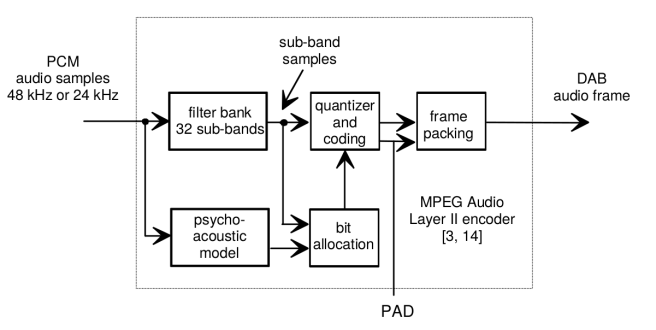
\includegraphics[width=.7\textwidth]{pic/mpeg2.png}
    \caption{Blokové schéma MPEG Layer II v systému DAB. \cite{web:mp2} }
    \label{pic:mp2}
\end{figure}

Vstupní pulzně kódovaný signál je rozdělen do dvou cest. V první z nich se nachází banka třiceti dvou filtrů, dělících signál do frekvenčních subpásem, která jsou poté kódována nezávisle. Blok zvaný psychoakustický model využívá principu zvaného spektrální sluchové maskování, neboli schopnosti lidského mozku nevnímat určité kmitočty, zní-li současně s nimi kmitočty jiné. Výstup tohoto bloku říká, jak hrubě kvantizovat (úrovňově rozdělit) jednotlivá subpásma.

Na takto upravené datové toky je poté použito Huffmanovo kódování, které častěji se vyskytujícím datovým slovům přiděluje kratší kódová slova. Tento princip je známý například z Morseovy abecedy. Konečnou fází je \uv{balení} dat do rámců a opatření hlavičkou obsahující data nezbytná pro dekodér.
 
\subsection{Advanced Audio Coding}

Standard AAC, přestavený jako součást specifikace MPEG-2, později doplněný o nové profily v MPEG-4 \cite{iso:aac} a MPEG-D je rodinou kodeků, která si klade za cíl poskytnout lepší poslechovou kvalitu, než \textit{mp3} při použití stejného bitového toku. Je postaven na modulárním přístupu. Podle potřeby lze využít různých rozšíření základního profilu a tím dosáhnout lepšího kódového zisku, efektivnějšího kódování řeči nebo například nižšího zpoždění. Na obrázku \ref{pic:aac} je naznačeno jakým způsobem jsou vrstveny profily používané v digitálním rádiu, popsané v následujících podkapitolách.

\begin{figure}[h]
    \centering
    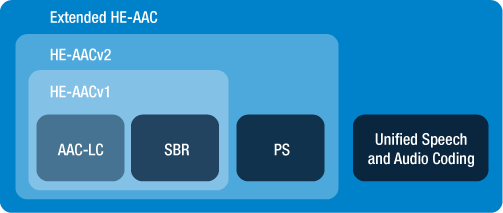
\includegraphics[width=.5\textwidth]{pic/aac.png}
    \caption{Grafické znázornění vzniku jednotlivých profilů kodeku AAC postupným přidáváním moderních technologií zpracování zvuku. \cite{web:voiceage} }
    \label{pic:aac}
\end{figure}

\subsubsection{Low Complexity}

Z funkčního hlediska dosahuje AAC oproti starším kodekům vyššího kódového zisku pomocí několika strategií. Kompletní blokové schéma AAC kodéru převzaté ze standardu ISO 13818-7 \cite{iso:aac} se nalézá na obrázku \ref{pic:aaclc}.

\begin{figure}[h]
    \centering
    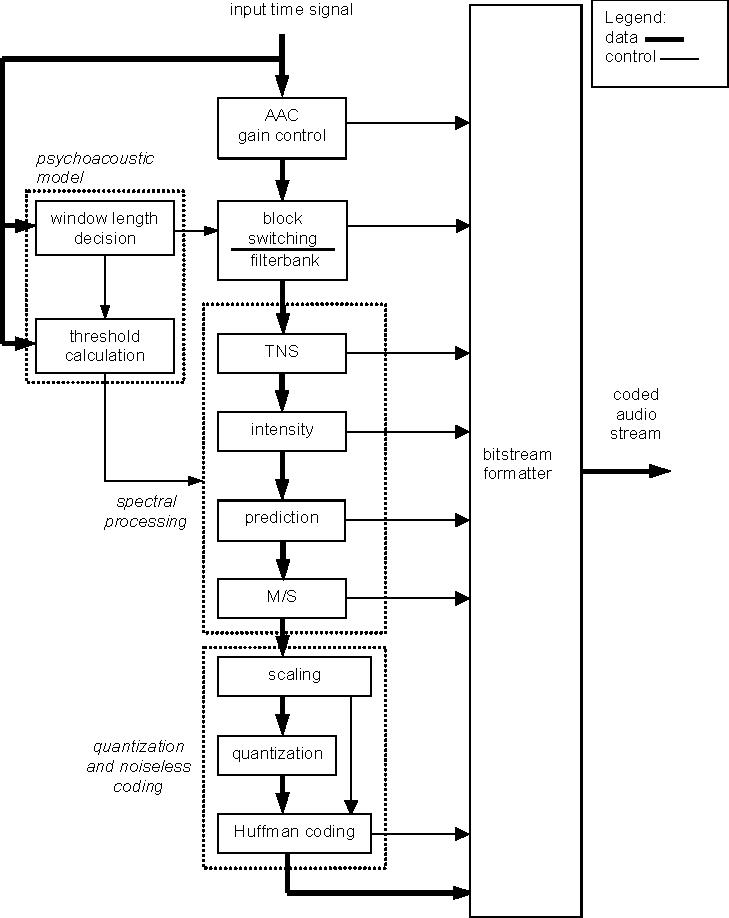
\includegraphics[width=.7\textwidth]{pic/aaclc.pdf}
    \caption{Blokové schéma AAC kodéru převzaté z normy \cite{iso:aac}}
    \label{pic:aaclc}
\end{figure}

Místo dělení signálu do několika desítek pásem pomocí filtrů v časové doméně, používá AAC LC profil modifikovanou\footnote{Modifikace transformace spočívá v úpravě transformačního jádra. Původně kosinový tvar se přibližuje obdélníkovému pulzu} kosinovou transformaci MDCT (\textit{Modified discrete cosine transform}) s proměnlivě dlouhými bloky. Ta je použita k převodu záznamu do 1024 frekvenčních subpásem, které jdou selektivněji kvantizovat výstupem psychoakustického modelu. Dále využívá vyrovnávací paměť pro zpětné adaptivní kódování. Pokud se v paměti kodéru nachází sekvence bitů, která je zrovna na vstupu, uloží se na výstup pouze její adresa. Jedná se o podobný přístup jako známé I, P a B snímky v pohyblivém obraze. V neposlední řadě používá AAC techniky jako jsou například TNS (\textit{Temporal Noise Shaping}), která \uv{posouvá} kvantizační šum nad slyšitelné pásmo, či JS (\textit{Joint Stereo}), které místo dvou plných kanálu ukládá jejich součet a jejich rozdíl, což je z hlediska entropie dat efektivnější.

Maximální bitová rychlost AAC závisí na vzorkovacím kmitočtu. Pro 44.1 kHz je to 264.6 kb/s, pro 48 kHz 288 kb/s. \cite{iso:aac}


\subsubsection{High Efficiency v1}

Vyšší kmitočty zabírají v tradičním kódování audiosignálů poměrně velkou část uložených dat. Ukazuje se ovšem, že z psychoakustického hlediska je exaktní reprodukce posledních jedné až dvou oktáv relativně nedůležitá. Při pouhém potlačení vyšších kmitočtů dolní propustí, jako to dělaly starší kodeky při nedostatečném datovém toku, ovšem označují posluchači vjem jako \uv{neúplný} či \uv{dutý} i přes zachování většiny relevantní informace. To společně s faktem, že z fyzikálního hlediska produkují hudební nástroje zvuky na ve spektru se periodicky opakujících kmitočtech, známých jako vyšší harmonické, vedlo k myšlence spektrální pásmové replikace (\textit{Spectral Band Replication}). Obrázek \ref{pic:sbr} naznačuje, jak takový proces probíhá na straně dekodéru. Pomocí transpozice je základní spektrum \uv{překopírováno} do pásma vyšších kmitočtů a poté je upravena spektrální obálka podle SBR dat vzniklých při kódování dat vstupního signálu. 

\begin{figure}[h]
    \centering
    \begin{subfigure}{.5\textwidth}
        \centering
        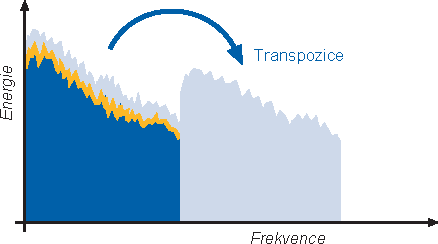
\includegraphics[width=1\linewidth]{pic/sbr1.pdf}
        \caption{Doplnění vyšších kmitočtů transpozicí.}
        \label{fig:sub1}
    \end{subfigure}%
    \begin{subfigure}{.5\textwidth}
        \centering
        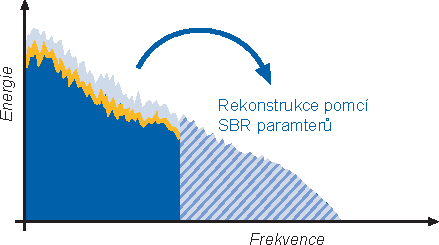
\includegraphics[width=1\linewidth]{pic/sbr2.pdf}
        \caption{Úprava energetické obálky.}
        \label{fig:sub2}
    \end{subfigure}
    \caption{Proces spektrální pásmové replikace.\cite{article:aac}} 
\label{pic:sbr}
\end{figure}
    
Při opětovném pohledu na obrázek \ref{pic:aac} vidíme, že kombinace AAC-LC v kombinaci se SBR tvoří profil známý pod jako \textit{High Efficiency AAC v1}. Tento princip obalování původního přístupu modernějšími technologiemi zajišťuje plnou zpětnou a částečnou dopřednou kompatibilitu.

Je nutno podotknout, že HE-AAC v1 není definován pro stejné bitové rychlosti jako jeho předchůdce. Při postupném snižování bitové rychlosti dostačuje kvalita \textit{Low Coplexity} profilu až do přibližně 128 kb/s. Při nižších datových tocích se již začíná být patrná přítomnost kompresních artefaktů. Snížení kvantizačního šumu lze dosáhnout pomocí zúžení pásma a právě tam nastupují výhody SBR.
    
\subsubsection{High Efficiency v2}
    
Profil známý jako HE-AAC v2 je dalším evolučním krokem v rodině kodeků AAC. Nad jeho předchozí verzi staví proces známý jako Parametrické Stereo PS (\textit{Parametric Stereo}). Podobně jako u SBR, které namísto původních dat využívá parametrického popisu obálkou, používá parametrické stereo signálovou podobnost. Tentokrát nikoli v kmitočtovém spektru ale v čase. Kodér ze vstupního signálu vezme levý a pravý kanál a smíchá je do jednoho \uv{monoaurálního} kanálu, jak naznačuje obrázek \ref{pic:ps}. Dále vypočítá z obou původních kanálů tři následující parametry:

    \begin{figure}[h]
        \centering
        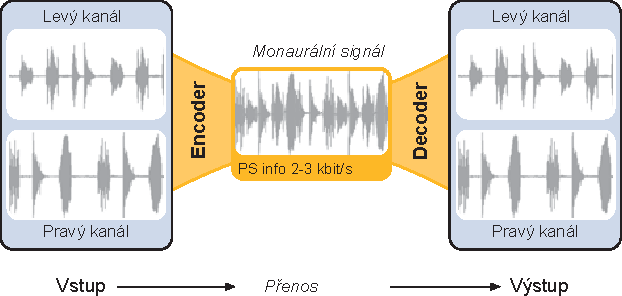
\includegraphics[width=.7\textwidth]{pic/parametricalStereo.pdf}
        \caption{Parametrické stereo \cite{article:aac}}
        \label{pic:ps}
    \end{figure}
    
    \begin{itemize}
        \item IID \textit{Inter-channel Intensity Difference} - Popisující rozdíl intenzity mezi jednotlivmi kanály. 
        \item ICC \textit{Inter-channel Cross-Correlation} - Vyjadřující míru koherence mezi jednotlivými kanály. Je vypočítán korelační funkcí.
        \item IPD \textit{Inter-channel Phase Difference} - Určující míru \uv{zpozdění} jednoho signálu vůči druhému.
    \end{itemize}
    
I tento profil se používá až při rychlostech, kdy již kvalita předchozích dvou profilů není dostatečná. 64 kb/s je maximální bitová rychlost při které lze parametrické stereo použít.
    
    \subsubsection{MPEG-D USAC}
    
Ať už jde o předčítání zpráv, diskuzní pořady či krátké vstupy moderátora mezi hudební reprodukcí, mluvené slovo je v rádiu velmi častým prvkem. Dlouhodobý vývoj přenosu řeči skrze digitální telefonní linku přineslo efektivní kódování mluveného slova zvané LPC (\textit{Linear Predictive Coding}). Vychází z poznatků o rezonanci zvukových vln v dutinách a dekompozici lidské řeči na elementy, které lze popsat databází. Na lidské hlasové ústrojí lze pohlížet jako na soustavu rezonančních trubic, ve kterých jsou zesíleny určité kmitočty, udávající barvu lidského hlasu. LPC analýza pomocí filtrů oddělí tyto kmitočty a vytvoří parametrický popis barvy hlasu. Ve zbytku signálu poté vyhledá řečové elementy a přiřadí jim prvky z databáze, kterou disponuje kodér i dekodér. Na přijímající straně je poté možno zrekonstruovat velmi věrně znějící repliku původního hlasu.

MPEG-D USAC (\textit{Unified Speech and Audio Coding}) vznikl myšlenkou spojit řečové AMR-WB+ (\textit{Extended Adaptive Multi-Rate – Wideband}) a hudební HE-AAC v2 kódování. Standard ISO/IEC 23003-3, známý pod označením MPEG-D, definuje nový přírůstek do rodiny AAC kodeků s názvem xHE-AAC (\textit{eXtended High Efficiency Advanced Audio Coding}) \cite{iso:usac},který cílí na bitové rychlosti 32 kb/s a nižší. Při pohledu na obrázek \ref{pic:aac} se může zdát, že xHE-AAC je jen dalším rozšířením, postaveným nad HE-AAC v2. Ve skutečnosti to tak ale není. USAC využívá stejných technologií jako jeho předchůdce, ale redefinuje většinu bloků aby bylo možné využít LPC analýzu. 

    \begin{figure}[h]
        \centering
        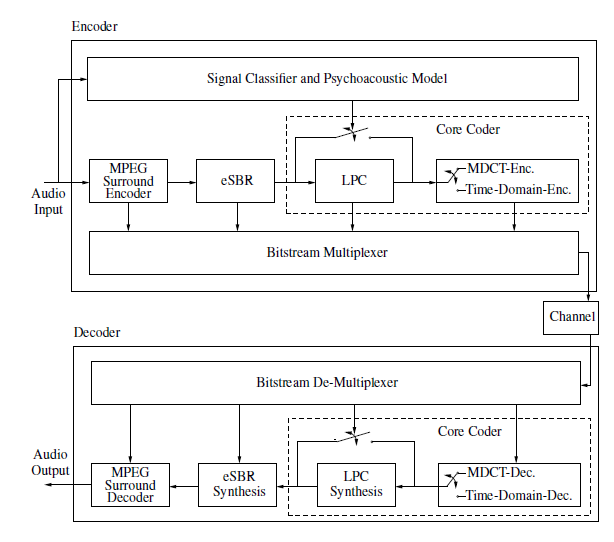
\includegraphics[width=.7\textwidth]{pic/usac.png}
        \caption{Kodér a dekodér xHE-AAC \cite{article:usac}}
        \label{pic:usac}
    \end{figure}
    
Na obrázku \ref{pic:usac} je naznačeno, jak kodek nakládá se vstupním signálem. Blok MPEG Surround produkuje parametrický popis stereofonního signálu a míchá kanály do jedné stopy. Ta je poté zpracována blokem eSBR (\textit{enhanced Spectral Band Replication}), který SBR použité v HE-AAC v2 doplňuje o efektivnější prediktivní vektorové kódování PVC (\textit{Predictive Vector Coding}). Jednokanálový nízkofrekvenční signál je poté po blocích zpracováván MDCT analýzou obdobnou té v Low Complexity profilu s volitelně doplněnou o LPC kodér. Volba přemostění řečového kódování lze vynutit natrvalo, či lze vypínat automaticky výstupem psychoakustického modelu rámec po rámci. Skokové přepínání mezi signálem kódovaným by mohlo produkovat kompresní artefakty. xHE-AAC proto definuje komplexní schéma přepínání mezi jednotlivými kódovacími metodami naznačené na obrázku \ref{pic:usac:switching}.

    \begin{figure}[h]
        \centering
        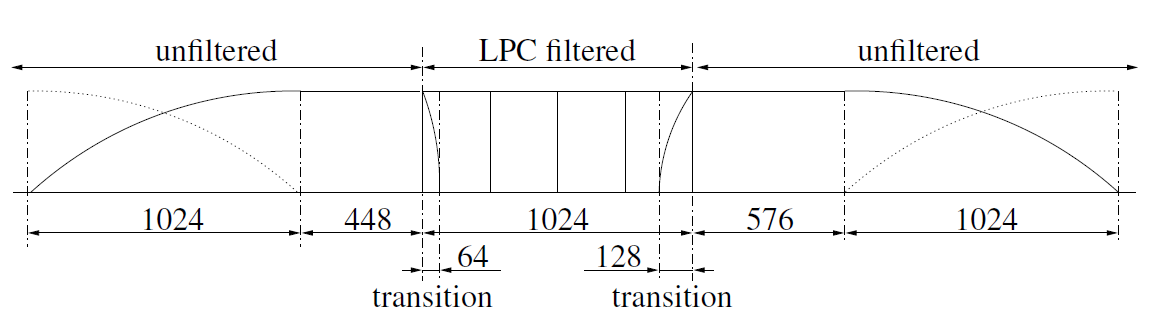
\includegraphics[width=.6\textwidth]{pic/switching.png}
        \caption{Schéma přepínání módů v USAC \cite{article:usac}}
        \label{pic:usac:switching}
    \end{figure}


\subsection{Opus}

Částečně mimo celou koncepci této práce stojí kodek jménem Opus. DAB ani DRM ho nemají ve svých definicích, i když na fóru \textit{HydrogenAudio} \cite{forum:hydro} jsou k nalezení zmínky tom, že s jistými úpravami lze Opus v DRM používat. To je nicméně velmi okrajová varianta a není důvodem proč je ve zdejším výčtu uveden. Skutečným důvodem pro jeho volbu byla jeho dostupnost. Je totiž jediným volně dostupným kodekem využívajícím sjednocené kódování řeči a hudby USAC. Srovnání s xHE-AAC by tedy mohlo být zajímavé.

Opus je standardizován pod záštitou IETF \textit{(Internet Engineering Task Force)} jako RFC6716 \cite{norm:opus}. Je relativně nový tj. jeho vývoj započal v roce 2007 a první verze spatřila světlo světa 11. Září 2012. V oficiálních materiálech autoři poskytují srovnání s velkým množstvím v současnosti používaných kodeků (obrázek \ref{pic:opus}), kde si vede velmi dobře.


\begin{figure}[h]
    \centering
    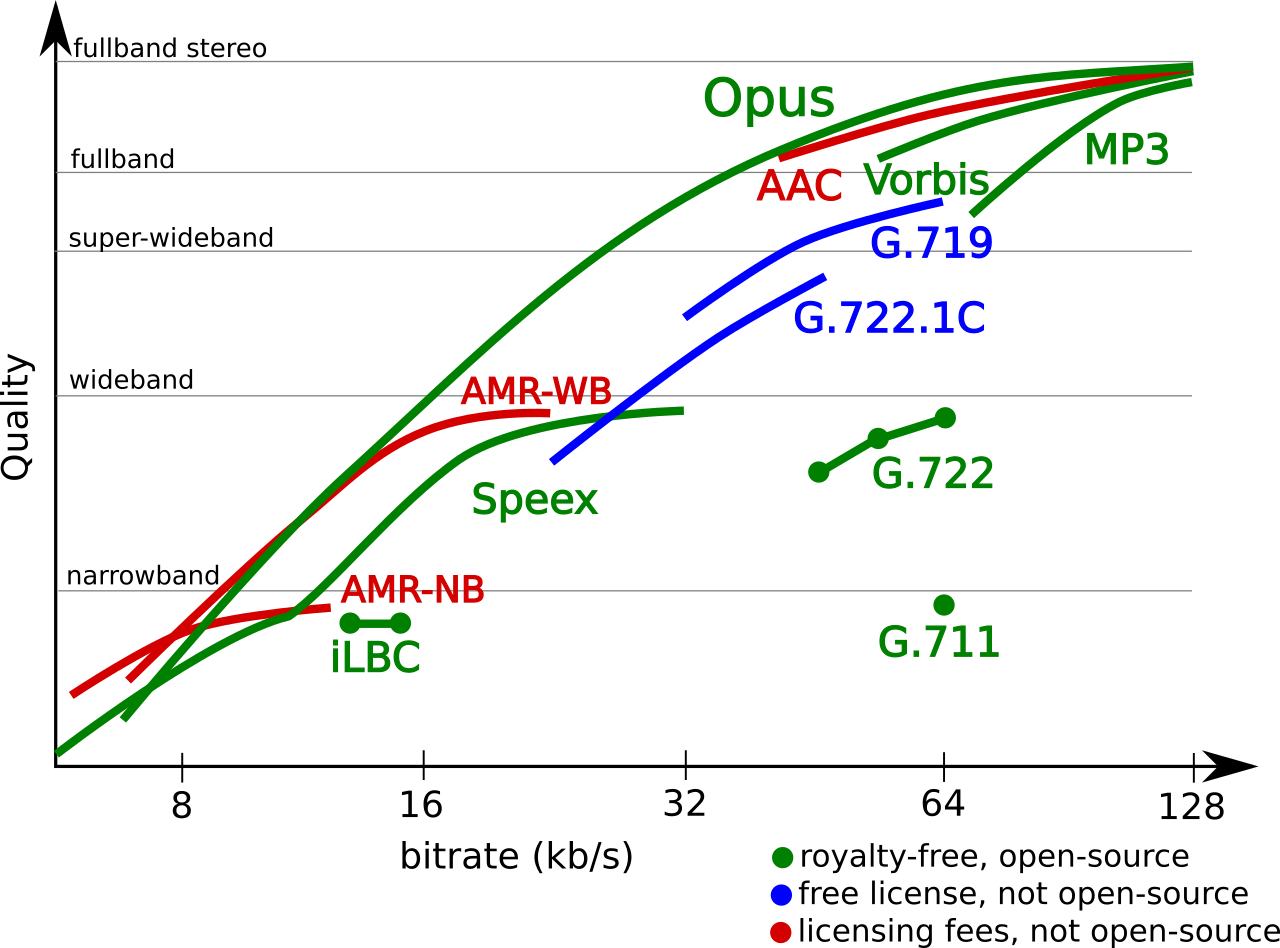
\includegraphics[width=.55\textwidth]{pic/opus.png}
    \caption{Srovnání kodeku Opus s ostatnímu kompresními metodami podle \cite{web:opus}}
    \label{pic:opus}
\end{figure}

Z technologického hlediska se velmi podobá xHE-AAC. Tam kde MPEG utilizuje řečové kódování AMR-WB+, využívá Opus kodek SILK vyvinutý společností Skype Technologies pro internetovou telefonii. Ke kódování zvuku používá CELT (\textit{Constrained Energy Lapped Transform}) otevřený kodek založený, stejně jako AAC, na MDCT analýze \cite{norm:opus}.
\chapter{Poslechové testy}
\label{chap.listeningTests}

\epigraph{\hfill\textit{Nejkrásnější hudba je lidský smích.}}{Jan Werich}


Do dnešních dní jsou subjektivní poslechové testy nejvěrohodnějším způsobem hodnocení kvality ve zvukové technice. V průběhu let vydala Mezinárodní telekomunikační unie řadu doporučení, podrobně popisujících různé druhy poslechových testů, jejich metodiky, zaměření, podmínky za jakých mohou být prováděny, jakým způsobem je vyhodnocovat atd. Akademická obec se jich drží, jelikož test provedený podle doporučení ITU má oproti testům nestandardizovaným zaručenou výpovědní hodnotu.

%\section{Druhy Testů}

Z nepřeberného množství doporučení, jenž ITU-R definuje, se dají vybrat tři normy bezprostředně se týkající subjektivního testování. Seřazeny dle doby vydání jsou to následující:

\begin{enumerate}
    \item Metoda pro nepatrná zhoršení:  ITU-R BS.1116 \cite{itur:1116}
    \item Obecné metody testování: ITU-R BS.1284 \cite{itur:1284}
    \item Metoda pro střední kvalitu, známá pod označením MUSHRA: ITU-R BS.1534 \cite{itur:1534}
\end{enumerate}

Na následujících řádcích je uveden rámcový popis jednotlivých metod vyjma testu typu MUSHRA, který je ze všech metod popsán nejpodrobněji, jelikož je v praktické části využit pro testování kvality komprimovaných souborů.


\section{Metoda pro nepatrná zhoršení}

\label{subchapter:impairment}

Anglicky \textit{Small impairments method} popsaná v \cite{itur:1116} cílí na aplikace, kde lze sledovat zhoršení, které může být nepostřehnutelné bez splnění přísných podmínek a bez důkladné statistické analýzy. Své využití nalézá například při vývoji reprodukčních zařízení či návrhu nových kodeků.

Subjekty musí být tak zvaní znalí posluchači (\textit{expert listeners}) neboli lidé, u nichž je předchozími testy prokázáno, že nedisponují žádnou sluchovou vadou. Před samotným testováním musí projít důkladným výcvikem. Taktéž jsou z výsledků vyřazeny všechny výsledky, jenž neodpovídají přísným kritériím, které doporučení definuje.

Při samotném průběhu testování se využívá přístup anglicky zvaný \textit{The double blind triple stimulus with reference}, neboli dvojitě slepý test se třemi podněty včetně známé reference. Subjektu jsou prezentovány tři stimuly. Referenční označovaný \uv{A} a dva neznámé s označením \uv{B} a \uv{C}, z nichž jeden je stejný jako známá reference a druhý je signál testovaný. Pojmem \uv{nepatrné zhoršení} se myslí jakákoliv odlišnost od původního signálu. Úkolem subjektu je tuto odlišnost odhalit a ohodnotit na škále v tabulce \ref{table:impairment}. Průměr udělené známky je v anglicky psané literatře označován jako $MOS$ (\textit{Mean Opinion Score}).

Udělení známky jednomu vzorku se říká zkouška. Test se skládá minimálně z pěti takovýchto zkoušek, kde délka podnětu nepřesahuje 25 vteřin. Celé sezení by ovšem nemělo přesáhnout třicet minut, aby případná únava subjektu neovlivnila jeho hodnocení. Po udělení známky se bez prodlení postupuje k další zkoušce.

Samotné vzorky by měly být vybrány tak aby reflektovaly zkoumanou problematiku a zároveň by si měly zachovat dostatečnou rozmanitost. Tj. je-li sledována kvalita mluveného slova, je třeba dbát na rozmanitost barev hlasů, rychlosti předčítání, pohlaví interpreta apod. Kapitola 8 doporučení \cite{itur:1116} \uv{Poslechové podmínky} (\textit{Listening conditions}) definuje, jakým způsobem by měl být posluchačům zvukový materiál prezentován. V nejlepším případě by měl být test proveden v poslechové místnosti s definovanými parametry jakými jsou například: objem a rozměry místnosti, doba dozvuku, referenční reprodukční zařízení atd. Pokud poslechová místnost není k dispozici, lze k testování využít referenčních sluchátek\footnote{Definici referenčních sluchátek se důkladněji věnuje podkapitola \ref{subchapter:devices}.}. Hluk na pozadí ovšem nesmí překročit hladinu, která by subjekty rušila při poslechu.

Výsledky testů podle tohoto doporučení se prezentují na stupnici v anglosaské literatuře známé jako $SDG$ (\textit{Subjective Difference Grade}). Hodnota $SDG$ se získá rozdílem udělených známek testovanému a referenčnímu signálu (rovnice \ref{equation:sdg})

\begin{equation}
    SDG = \text{Známka}_{testovaný} - \text{Známka}_{referenční}
    \label{equation:sdg}
\end{equation}


\begin{table}[h]
\centering
\begin{tabular}{|c|c|c|}
\hline
Zhoršení       & Známka ($MOS$) & $SDG$  \\ \hline
Nepostřehnutelné              & 5 & 0  \\ \hline
Postřehnutelné, avšak neruší & 4 & -1 \\ \hline
Mírně rušivé       & 3 & -3 \\ \hline
Rušivé              & 2 & -4 \\ \hline
Velmi rušivé        & 1 & -5 \\ \hline
\end{tabular}
\caption{Hodnotící škála podle \cite{itur:1116} (Překlady z \cite{book:melka})}
\label{table:impairment}
\end{table}

\section{Obecné metody}

Protože doporučení \cite{itur:1116} je v některých ohledech velice striktní, vydala ITU doplňující standard, ve kterém shrnuje další v praxi využívané metody. Definovala pro ně hodnotící škály, parametry prostředí ve kterém testy realizovat a podmínky, které by měli splňovat subjekty testy provádějící.

\subsection{Párové srovnávání}

V této metodě, známé také jako \uv{AB Test} volí subjekt jeden ze dvou stimulů označených \uv{A} a \uv{B}. Test může být koncipován tak, že je hledán poslechově přívětivější podnět, či je rozdíl těchto dvou stimulů označen na hodnotící škále. Doporučení rovněž říká, že jeden ze dvou podnětů může, ale nemusí být referenční.

Hodnotících škál je v doporučení popsáno hned několik. Pro případ že je sledováno zhoršení, využívá se stejného známkování jako v tabulce \ref{table:impairment}. Vyskytují-li se při hodnocení vzorky jak horší tak lepší, měla by být použita následující stupnice.

\begin{table}[h]
\centering
\begin{tabular}{|c|c|}
\hline
Zhoršení       & Známka \\ \hline
Mnohem horší              & -3      \\ \hline
Horší & -2      \\ \hline
Trochu horší       & -1      \\ \hline
Stejné              & 0      \\ \hline
Trochu lepší        & 1      \\ \hline
Lepší        & 2      \\ \hline
Mnohem lepší        & 3      \\ \hline
\end{tabular}
\caption{Bipolární škála podle \cite{itur:1284} (Překlady z \cite{book:melka})}
\label{table:bipolarscale}
\end{table}

Zda bude škála využita či nikoli záleží na sledovaných parametrech. Je-li třeba znát kvalitativní rozdíly mezi jednotlivými stimuly, je užití škály doporučeno. Hledá-li se pouze jeden vzorek s žádoucími parametry, stačí známkování typu \uv{lepší/horší}. 

Je doporučeno, ale ne vyžadováno, aby subjekty byli z řad znalých posluchačů. Pokud to není možné, měli by minimálně projít tréninkem, aby se seznámili s testovací procedurou. Co se poslechových podmínek týče, odvolává se norma na předchozí doporučení \cite{itur:1116}.

\subsection{Seřazování do pořadí}

Ve volbě posluchačů a dodržování reprodukčních podmínek se tato metoda neliší od předchozí. Metodika je ovšem jiná. Subjektu je v rámci jedné zkoušky představeno podstatně větší množství podnětů. Typicky pět až devět. Posluchač poté přiřazuje hodnocení subjektivně vnímané kvality na spojité stupnici $CQS$ (\textit{Continuous Quality Scale}), popsané tabulkou \ref{table:cqs}. Numerickou hodnotou od nuly do sta, či vyznačením bodu na úsečce udělí hodnocení každému z prezentovaných stimulů. Nemělo by být dovoleno udělit stejnou známku dvěma stejným podnětům.

\begin{table}[h]
\centering
\begin{tabular}{|c|c|c|}
\hline
Interval & Slovní popis anglicky & Slovní popis česky \\ \hline
80 \% - 100 \% & Excellent & Vynikající \\ \hline
60 \% - 80 \% & Good & Dobrá \\ \hline
40 \% - 60 \% & Fair & Přijatelná \\ \hline
20 \% - 40 \% & Poor & Špatná \\ \hline
0 \% - 20 \% & Bad & Nepřijatelná \\ \hline
\end{tabular}
\caption{Unipolární sto-dílková škála CQS pro popis kvality se slovními popisy dle \cite{itur:1284} a překlady z\cite{book:melka})}
\label{table:cqs}
\end{table}

\section{Metoda pro střední kvalitu}

Doporučení \cite{itur:1534} definuje tzv. Vícestimulový test se skrytou referencí a kotvou MUSHRA (\textit{MUltiple Stimuli with Hidden Reference and Anchor}). Jedná se o metodu navrženou přímo pro hodnocení kvality výstupu ztrátových kodeků. Využití tedy nalézá při hledání optimálních parametrů pro přenos zvuku v internetových službách, rádiích či televizním vysílání.

\subsection{Metodika} 

Podobně jako při seřazovacím testu je při provádění testu MUSHRA posluchači při jedné zkoušce představeno vetší množství podnětů. Typicky deset, maximálně však patnáct. První z nich je vždy známý, nezkreslený vzorek a ostatní náhodně zamíchané testované stimuly, mezi které je náhodně vložen skrytý referenční vzorek a jedna, či více kotev. Typy vzorků jsou podrobněji popsány v podkapitole \ref{subchapter:stimuli}. Posluchač hodnotí každý stimul na již předem zmíněné sto-dílkové CQS škále naznačené na obrázku \ref{table:cqs}. Opětovné přehrání kteréhokoliv stimulu by mělo být umožněno. 

\subsection{Výběr subjektů}

I přes to že test MUSHRA neslouží k detekci nepatrných zhoršení doporučuje standard vybírat subjekty z řad znalých posluchačů stejně jako doporučení \cite{itur:1116}. Minimalizuje se tím možnost chyby, kterou do testu může vnést subjekt vyplňující poslechový test bez předchozích zkušeností. Výběr posluchačů, jejichž hodnocení bude mít vliv na výsledky pokusu by měl být proveden na základě těchto dvou metod:

\begin{itemize}
    \item Pre-screening
    
    Předtest či forma zaučení, jejíž cílem je objevit, zda posluchač disponuje tzv. normálním sluchem\footnote{Co je normální sluch definuje ISO 389} a zda dokáže hodnotit zvuk kriticky.
    
    \item Post-screening
    
    Výběr subjektů na základě výsledků již provedeného testování. Starší verze normy \cite{itur:1534} definuje dvě kategorie podmínek na základě kterých je možno vyřadit hodnoty hodnocení konkrétního subjektu a to
    
    \begin{itemize}
        \item  nekonzistence opakovaného hodnocení vzorku se stejnými parametry
        \item nekonzistence hodnocení v rámci množiny subjektů jako například přílišná extremizace hodnocení.
    \end{itemize}
    
    Nová verze normy \cite{itur:1534-3} dodává konkrétní podmínku z první kategorie a to doporučení vyřadit subjekty, jejichž hodnocení skryté reference je ve více než patnácti procentech nižší než 90\%.
    
\end{itemize}

\subsection{Tréninková fáze}

Před ostrou fázi testu je vhodné vložit tzv. zaučení, neboli fázi pro seznámení s rozhraním a stimuly. Subjektu by měly být představeny všechny možné druhy podnětů s konkrétním popisem. Vysvětlení jak při testu postupovat, jakým způsobem udělit hodnocení apod. Zaučení je možno provést buď formou instruktážního videa, doprovodných instrukcí na přiloženém návodě, či formou testu \uv{nanečisto}.

\subsection{Podněty}
\label{subchapter:stimuli}

Délka jednotlivých podnětů by neměla překročit dvacet sekund. Obvykle se volí úsek okolo deseti vteřin, potažmo taková doba trvání, aby celý test nepřesáhl délku třiceti minut.
Jak už název testu naznačuje každá zkouška obsahuje následující podněty:

\begin{itemize}
    \item Známá reference:\\Stimul označený slovem \uv{Reference} obsahující nezkreslenou nahrávku.
    
    \item Skrytá reference:\\Stimul obsahově shodný se známou referencí, náhodně zamíchaný mezi testované podněty. Slouží k takzvanému \textit{post-screeningu}. Posluchač by měl být schopen takovýto podnět identifikovat a udělit mu vynikající hodnocení (z čehož mimo jiné plyne, že alespoň jedno hodnocení v každé zkoušce by mělo mít hodnotu 100 \%). Pokud ho posluchač neodhalí a udělí mu opakovaně nízké kvalitativní hodnocení, měl by být při analýze výsledků vyřazen. 
    
    \item Skrytá kotva:\\ Minimálně jeden a nebo více uměle zkreslených vzorků, náhodně vložených mezi ty testované. Může podobně jako skrytá reference sloužit k \textit{post-screeningu} a jeho smyslem je ukotvit kvalitativní škálu \uv{zdola}. Doporučení \cite{itur:1534} říká, že alespoň jedna z kotev by měla být odvozena od referenčního vzorku aplikováním dolní propusti s následujícími parametry.
    
    \smallskip
    
    $f_c=3,5$ kHz
    
    Minimální útlum na 4 kHz = 25 dB
    
    Minimální útlum na 4,5 kHz = 50 dB
    
    Maximální zvlnění v propustném pásmu = $\pm$ 0,1 dB
    
    \smallskip
    
    \item Testované vzorky:\\
    Stimuly označené písmeny \uv{A}, \uv{B} a dále na které je aplikováno zkreslení a na nichž je zkoumána problematika. Kvůli vyhodnocení testu je seznam podnětů konzistentní přes všechny zkoušky, tj. i přes to, že každá zkouška obsahuje jinou nahrávku, je na ní pokaždé aplikována stejná paleta zkreslení (pomocí kompresních algoritmů, či jinak přidaných artefaktů).
    
\end{itemize}

\subsection{Poslechové podmínky}
\label{subchapter:devices}
Doporučení \cite{itur:1534} se odvolává na poslechové podmínky definované v \cite{itur:1116} a v \cite{itur:708}, tj volbu mezi poslechovou místností osazenou referenční reprosoustavou či sluchátky. Protože v praktické části této práce jsou využita sluchátka, je  v tomto textu přiblížena pouze tato možnost. 
\smallskip
Doporučení \cite{itur:708} říká, že sluchátka musí splňovat následující:
\begin{itemize}
    \item Časové zpoždění mezi kanály sluchátek nesmí přesáhnout dobu $t_{delay} = 20\mu s$.
    \item Frekvenční charakteristika musí být plochá tzn. $G_{DS}$ (Odezva sluchátek v difuzním poli) musí ctít masku na obrázku \ref{pic:headphones}.
\end{itemize}

%\textcolor{red}{Zeptat se Runda na charakteristiku sluchátek}



\begin{figure}[ht]
    \centering
    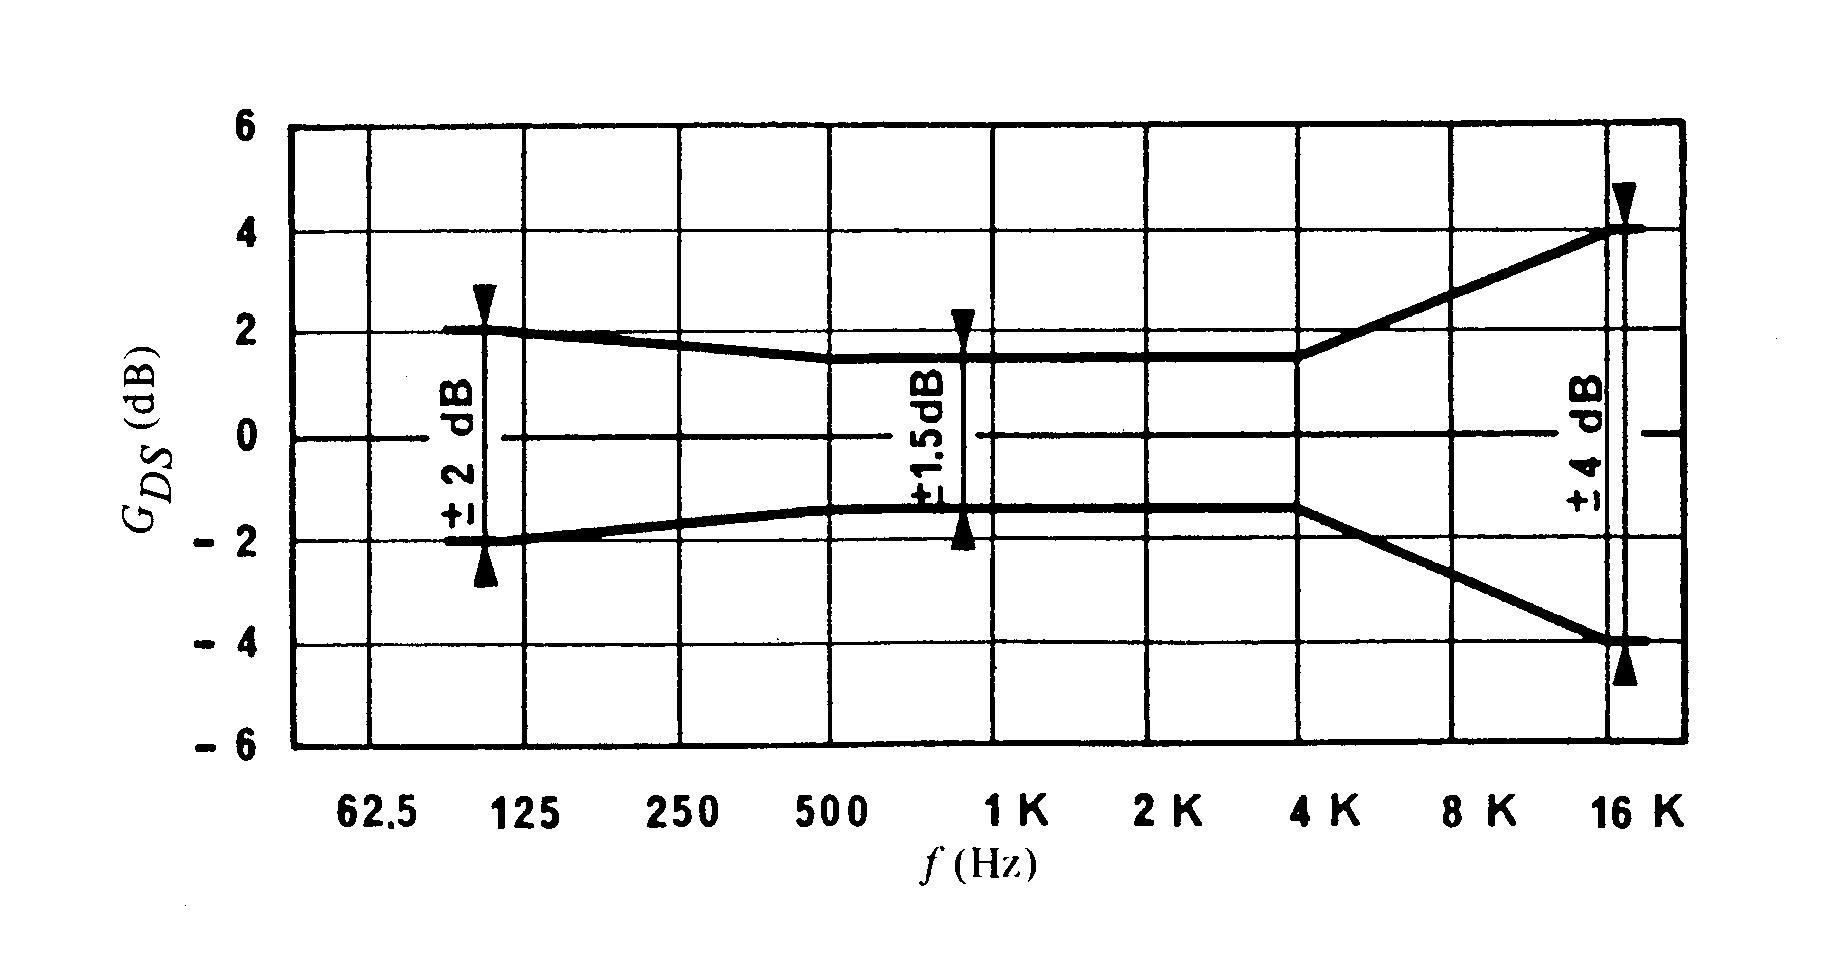
\includegraphics[width=.8\textwidth]{pic/headphones.png}
    \caption{Frekvenční toleranční maska studiových sluchátek z \cite{itur:708}}
    \label{pic:headphones}
\end{figure}


Samozřejmostí je, že všichni účastníci testu musí použít stejné poslechové zařízení.

\subsection{Statistická analýza}

Samotné provedení testu by bylo zbytečné bez provedení správné analýzy získaných dat. Podle knihy Základy statistiky \cite{book:statistika} se množina subjektů, na kterých je prováděno testování označuje jako \uv{výběr}. Cílem pokusu ovšem není zjistit \uv{výběrový průměr}, nýbrž aproximaci pro celou množinu potenciálních posluchačů. Zavádí se tedy pojem interval spolehlivosti ve kterém s nejvyšší pravděpodobností leží takzvaný \uv{populační průměr}. Jeho kalkulaci zahájíme výpočtem výběrového průměru $\bar{u}_{jk}$:

\begin{equation}
    \bar{u}_{jk}=\cfrac{1}{N}\sum_{i=1}^{N}u_{ijk}
\end{equation}

\noindent kde, $u_{ijk}$ značí hodnocení uživatele $i$ ve zkoušce $j$ testované metody zhoršení $k$ a $N$ odpovídá množství subjektů. Obdobným způsobem lze spočítat průměry $\overline{u}_j$ či například $\overline{u}_k$ \\

Doporučení \cite{itur:1534} říká, že výsledky mají být prezentovány na 95\% intervalu s krajními body:

\begin{equation}
    [\bar{u}_{jk} - \delta_{jk},\bar{u}_{jk} + \delta_{jk}]
\end{equation}

\noindent kde $\delta_{jk}$ je padesát procent šířky intervalu spolehlivosti daného vztahem: 

\begin{equation}
    \delta_{jk} = t_{0,05}\cfrac{\sigma_{jk}}{\sqrt{N}}
    \label{equation:inteval}
\end{equation}

\noindent a $t_{0,05}$ je hodnota odpovídající 95\% koeficientu spolehlivosti a stupni volnosti $N-1$, kterou lze najít ve statistických tabulkách. Směrodatná odchylka se poté spočítá podle:

\begin{equation}
    \sigma_{jk} =\sqrt{\sum_{i=1}^{N}\cfrac{(\bar{u}_{jk}-u_{ijk})^2}{N-1}}
\end{equation}
 
Vypočtením těchto hodnot zjistíme, že hodnota populačního průměru se nachází v intervalu spolehlivosti s pravděpodobností 95\%.



\subsection{Prezentace výsledků}

Zpracované výsledky by měly být prezentovány takovou formou, aby jim porozuměl jak laik tak expert v oboru. Na přehledném místě v textu by měl čtenář zprvu narazit na grafické zpracování s vyobrazeným intervalem spolehlivosti. To by mělo být doprovázené popisem toho co jednotlivé grafy vyjadřují nicméně není potřeba uvádět veškeré výpočty vedoucí k daným závěrům. Pokud je autor uvést chce, může je přiložit ve formě dodatku.
\smallskip

Opomenuto by tedy nemělo být následující: \begin{itemize}
    \item grafická reprezentace dosažených výsledků
    \item popis množiny subjektů: počet, průměrný věk..
    \item specifikace poslechového materiálu včetně důvodu pro výběr
    \item charakteristika poslechové místnosti včetně rozměrů, typy měničů, jejich umístění a konfigurace 
    \item popis metodiky testu
    \item způsob zpracování dat
    \
\end{itemize}
\chapter{Objektivní metody hodnocení kvality zvuku}
\label{chap:objectiveMetods}

\epigraph{\hfill\textit{Práce je to, co nikdo nechce dělat.}}{Tomáš Garrigue Masaryk}

Jak už je naznačeno v úvodu, objektivní algoritmy slouží jako alternativa k subjektivním poslechovým testům. Jde o způsob jakým obejít mnohdy náročné testování s velkým počtem posluchačů a tím ušetřit nemalé množství materiálních i časových prostředků.

Snaha o objektivní hodnocení za použití výpočetních metod se dá vysledovat až k počátkům devadesátých let. Existuje několik metod a pohledů na tuto problematiku, nicméně všechny v jádru sdílí obdobný přístup. Konkrétně snahu o modelování lidské sluchové cesty, dále přepočet na vnitřní koeficienty reprezentující nervové vzruchy a v závěru jejich matematické zpracování, často označované jako kognitivní analýza. Výsledkem bývá numerická hodnota odpovídající umístění na hodnotící škále, stejně jako tomu je při subjektivním testování.

V čem se metody liší je jejich zaměření a oblast použití. Telekomunikační sekce ITU-T, která standardizuje systémy jejichž cílem je přenést lidský hlas, se zabývá algoritmy, které sledují převážně srozumitelnost. Naproti tomu hodnocení v systémech definovaných radiokomunikační sekcí ITU-R se soustředí spíše na věrohodnost reprodukce originálního signálu v audiovizuálních systémech.

Dále by se metody daly rozdělit podle toho, zda pro svou funkci vyžadují referenci v plné kvalitě či nikoliv na tzv. \uv{Intruzivní} a \uv{Neintruzivní}. Vyhodnocování kvality řeči bývá častěji řešeno neintruzivně, jelikož algoritmy porovnávají testovaný materiál s vnitřními modely řeči. Hudba, která je zvukově \uv{rozmanitější} většinou vyžaduje přístup intruzivní.

\section{Metody užívané v telekomunikační technice}

I přes to že se tato práce nezabývá telekomunikační problematikou, je dobré zmínit jaké metody objektivního hodnocení kvality poslechu mluveného slova existují. Ať už proto, že do jisté míry sdílí vnitřní filozofii s těmi z oblasti multimediální techniky, tak proto že vývoj některých algoritmů pro hodnocení kvality hudebních nahrávek vzešel právě z této oblasti. 

%\subsection{Algoritmy definované Mezinárodní telekomunikační unií}
%\begin{itemize}
%    \item PSQM, PESQ a POLQA
\subsection{PSQM, PESQ a POLQA}    
    Jsou tři po sobě jdoucí standardy popisují intruzivní algoritmy určené k hodnocení řeči v telekomunikacích. Společně s evolucí telekomunikačního řetězce se vyvíjely i systémy objektivního hodnocení, nicméně všechny tři staví na modelování sluchové cesty a následné kognitivní analýze.
    
    Nejstarší PSQM \textit{Perceptual Speech Quality Measure} popsaný v ITU-T P.861 \cite{itut:861} v roce 1996 se soustředí na oblast telekomunikačního pásma 300 Hz - 3,4 kHz. Signály převádí do frekvenční oblasti, kde pomocí filtrů reprezentujících bazilární membránu vytvoří aproximaci zvuku, který vnímá účastník telefonního rozhovoru. Následovným porovnáváním signálů jsou určeny tři parametry:
    \begin{itemize}
        \item Časově-frekvenční zvlnění (\textit{Time-Frequency Warping})
        \item Frekvenční zvlnění (\textit{Frequency Warping})
        \item Úrovňové zvlnění (\textit{Intensity Warping})
    \end{itemize}
    Jejich váhovaným rozdílem je vypočten parametr označovaný jako $QD$ (\textit{Quality Degradation}), který je mapován na škálu $MOS$ (\textit{Mean Opinion Score}), která se používá jako výstup subjektivních testů.
    
 %   \bigskip
    
    Jako hlavní problém při hodnocení systémem PSQM se ukázalo zpožďování řeči způsobené paketovým přístupem v telefonii. Novější standard PESQ (Perceptual Evaluation of Speech Quality) dle ITU-T P.862 \cite{itut:862} principiálně popsaný obrázkem \ref{pic:pesq} tuto nevýhodu odstranil přidáním bloku \textit{Time alignment}. Ten napřed rozdělí signál na krátké úseky, v telekomunikaci zvané promluvy, korelací obálek odhadne, zda je nutná korekce a pokud ano rozdělí promluvy na rámce dlouhé 64 ms a ty pomocí výsledku korelace po vzorcích seskládá tak, aby testovaný signál odpovídal referenčnímu.
    
    \begin{figure}[h]
        \centering
        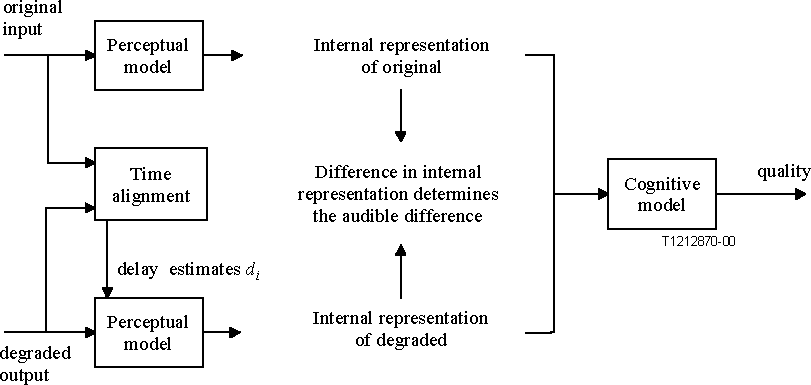
\includegraphics[width = .7\textwidth]{pic/PESQ.pdf}
        \caption{Blokové schéma algoritmu PESQ}
        \label{pic:pesq}
    \end{figure}
  
  %\bigskip
    
    Nejnovější metoda POLQA \textit{Perceptual Objective Listening Quality Assessment} dle ITU-T  P.863 z roku 2011 \cite{itut:863} řeší problematiku rozšiřovaní pásma použitého při přenosu telefonických hovorů. Definuje dva operační módy.
    \begin{itemize}
        \item Úzkopásmový: sloužící pro měření kvality v telefonním pásmu 300 Hz - 3,4 kHz. Pásmový ořez v tomto módu není považován za degradaci signálu a nemá vliv na objektivní hodnocení.
        \item Super-širokopásmový: ve kterém je šířka pásma rozšířena na 50 Hz - 14 kHz.
    \end{itemize}
    
    Princip hodnocení je podobný jako u předchozích modelů. Díky většímu výpočetnímu výkonu současných zařízení může POLQA sledovat více parametrů, a provádět složitější matematické operace při kognitivní analýze.
    
%    \item 3SQM
\subsection{3SQM}
    
    ITU–T P.563 \textit{Single Sided Speech Quality Measure} \cite{itut:536} je oproti dvěma předchozím algoritmům metodou intruzivní. Díky tomu lze využít kdekoliv v telekomunikačním řetězci a hodí se tak pro soustavné monitorování sítě. Principiální schéma je na obrázku \ref{pic:3sqm}.
    
    \begin{figure}[h]
        \centering
        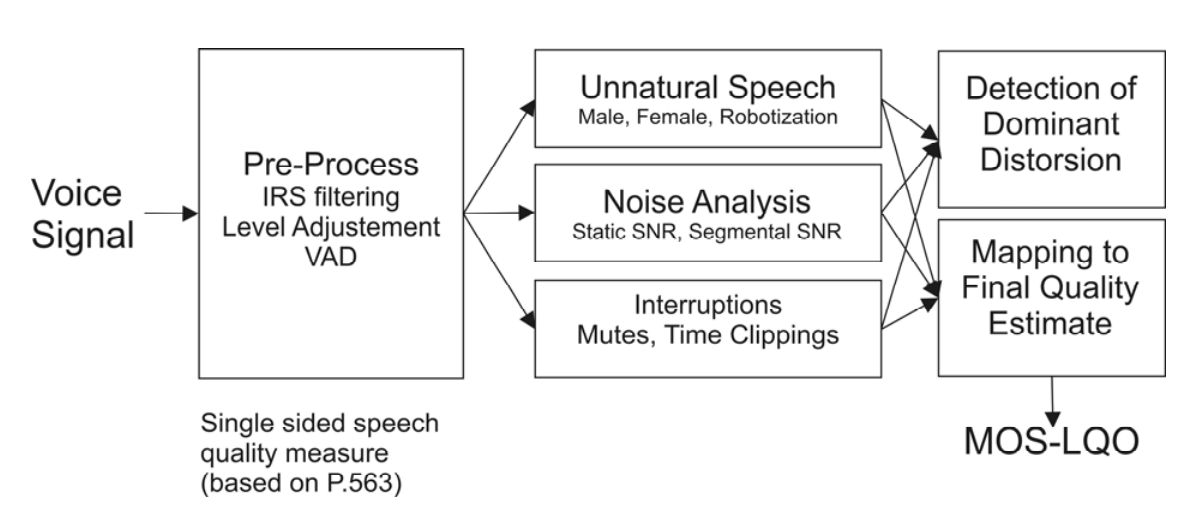
\includegraphics[width = .6\textwidth]{pic/3sqm.png}
        \caption{Blokové schéma algoritmu 3QSM}
        \label{pic:3sqm}
    \end{figure}

    Signál na vstupu prochází blokem předzpracování. Tím je normován a jsou z něj odstraněny rámce, které s řečí nesouvisí, pomocí tzv. IRS filtru (\textit{Intermediate Reference System}). Nehodí se tak pro detekci parametrů jako je zpoždění, ozvěny či poklesy hlasitosti, které mohou negativně působit na kvalitu telefonních hovorů. Samotná detekce probíhá porovnáváním úrovně obálky signálu.
    
    V signálu se poté sledují parametry jako výška hlasu, variace energie, nepřirozená periodičnost či různé druhy šumu. Na základě těchto parametrů je vytvořen pseudo-referenční signál, pomocí kterého je testovaný signál dále zpracováván intruzivním přístupem podobně jako v metodách PESQ či POLQA.
    
%\end{itemize}

\subsection{ViSQOL}
\label{subchapter:visqol}

\textit{The Virtual Speech Quality Objective Listener} je nástroj představený ve stejnojmenném článku v roce 2012 \cite{article:visqol}. Staví na intruzivním algoritmu zvaném NSIM (\textit{Neurogram Similarity Index Measure}), původně vyvíjeném pro řečovou predikci. Neurogram je analogií ke spektrogramu, kde intenzita barvy přestavuje sílu vzruchu neurální aktivity. Na obrázku \ref{pic:visqol} je naznačen tok dat algoritmem ViSQOL.

\begin{figure}[h]
    \centering
    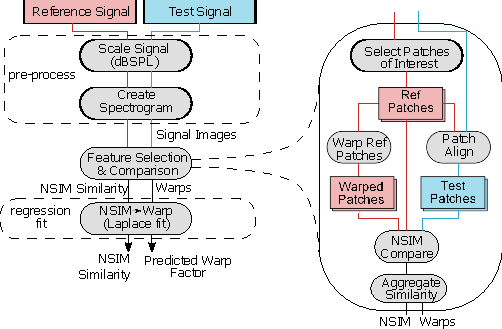
\includegraphics[width = .7\textwidth]{pic/visqol.pdf}
    \caption{Blokové schéma algoritmu ViSQOL\cite{article:visqol}}
    \label{pic:visqol}
\end{figure}

V první části označené jako předzpracování dochází k úrovňovému vyrovnání testovaného a referenčního signálu. Poté jsou pomocí Fourierovy krátkodobé transformace STFT oba signály převedeny na spektrogramy o třiceti frekvenčních pásmech logaritmicky rozdělených od 250 Hz do 8 kHz.

Část označená jako \textit{Feature Selection \& Comparsion} slouží k identifikaci vzájemně korespondujících políček\footnote{Anglicky označována jako \textit{patches}. Žádný dosavadní český překlad nebyl nalezen a z možností ve slovníku slovo políčko nejlépe významově koresponduje.}. Rozměr políčka je 30 rámců x 30 frekvenčních pásem. Algoritmus z obou zpracovávaných signálů vybírá tři takováto políčka nalezením maxima v pásmech 2, 6 a 10, se středními frekvencemi zhruba 250 Hz, 450 Hz a 750 Hz.
Poté je na korespondující políčka aplikována metoda výpočtu rozdílu pomocí kvadratické střední chyby\footnote{RMSE (Root Mean Squared Error)} rámec po rámci a pomocí minima této hodnoty jsou políčka zarovnána.

V posledním kroku se na políčka aplikuje NSIM, který vypočítá rozdílové skóre od nuly do jedné, kde nulové hodnocení dostávají signály bez jakékoli podobnosti a jedničku signály identické. Zároveň algoritmus vrací míru časového zkreslení (\textit{Time Warping}).

\section{Metody v multimediální technice}
\subsection{PEAQ}

\textit{Perceived Evaluation of Audio Quality} zkráceně PEAQ je objektivní metoda hodnocení vnímané kvality zvuku popsaná v ITU-R BS.1387-1 \cite{itur:1387}. Princip metody je zobrazen na obrázku \ref{pic:peaq}. Jedná se o intruzivní metodu, které je třeba dodat společně se zkresleným signálem signál referenční. Ty jsou převedeny do frekvenční oblasti. Jejich spektrální reprezentace prochází modelem slyšení a následně jsou z nich spočítány \textit{Model Output Values} zkráceně $MOV$. V závěru jsou v bloku zvaném \textit{Artificial Neural Network} provedeny výpočty simulující kognitivní procesy mozku. Výsledkem algoritmu je parametr zvaný $ODG$ (\textit{Objective Differemce Grade}), což je ekvivalent jednotky $SDG$, představené v podkapitole \ref{subchapter:impairment}

\begin{figure}[h]
    \centering
    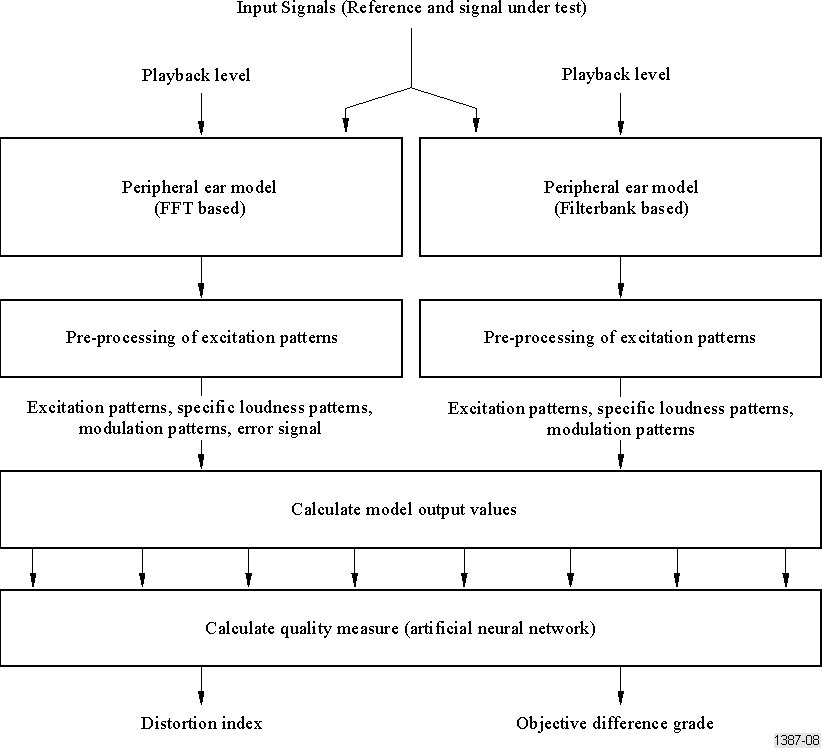
\includegraphics[width = .75\textwidth]{pic/peaq2.pdf}
    \caption{Blokové schéma algoritmu PEAQ}
    \label{pic:peaq}
\end{figure}

Model PEAQ existuje ve dvou verzích. Základní (\textit{Basic}) a pokročilé (\textit{Advanced}). Ta se od první liší především mírou komplexity výpočtů v sluchové a kognitivní části a použitím druhého modelu sluchové cesty založené na bance filtrů.

\begin{table}[h]
\centering
\begin{tabular}{|c|c|c|}
\hline
Název MOV & Model & Popis \\ \hline
\multicolumn{3}{|c|}{PEAQ Basic} \\ \hline
$BandwidthRef_B$ & FFT & Šířka pásma referenčního signálu \\ \hline
$BandwidthTest_B$ & FFT & Šířka pásma testovaného signálu \\ \hline
$Total NMR_B$ & FFT & Poměr Šum/Maska \\ \hline
$WinModDiff1_B$ & FFT & Váhovaný modulační rozdíl \\ \hline
$ADB_B$ & FFT & Průměrné blokové zkreslení \\ \hline
$EHS_B$ & FFT & Harmonická struktura chyb \\ \hline
$AvgModDiff1_B$ & FFT & Průměrný modulační rozdíl 1 \\ \hline
$AvgModDiff2_B$ & FFT & Průměrný modulační rozdíl 2 \\ \hline
$RmsNoiseLoud_B$ & FFT & Hlasitost zkreslení \\ \hline
$MFPD_B$ & FFT & Maximální vážená pravděpodobnost detekce \\ \hline
$RelDistFrames_B$ & FFT & Vzájemně zkreslené rámce \\ \hline
\multicolumn{3}{|c|}{PEAQ Advanced} \\ \hline
$RmsModDiff_A$ & Banka Filtrů &  \\ \hline
$RmsNoiseLoudAsym_A$ & Banka Filtrů & Hlasitost zkreslení \\ \hline
$Segmental NMR_B$ & FFT & Poměr Šum/Maska \\ \hline
$EHS_B$ & FFT & Harmonická struktura chyb \\ \hline
$AvgLinDist_A$ & Banka Filtrů & Lineární zkreslení \\ \hline
\end{tabular}
\caption{Seznam parametrů MOV}
\label{table:movs}
\end{table}

Algoritmus PEAQ předpokládá, že signály jsou vzorkovány kmitočtem 48 kHz a zároveň jsou časově a úrovňově vyrovnané. Po načtení je rozdělí do rámců o 2048 vzorcích s vzájemným 50\% překryvem. Dále je na rámce aplikováno Hannovo okno a pomocí diskrétní Fourierovy transformace jsou převedeny do frekvenční domény.

Model sluchové cesty se skládá z různých filtrů, reprezentace vnitřního šumu a výpočtu rozprostírání frekvenčních složek pomocí násobení bankou tzv \textit{Spreading functions}. Výstupem těchto matematických operací jsou $MOV$, jejichž seznam je v tabulce \ref{table:movs}.

Neuronová síť je rovnice \ref{equation:peaq}, do které vstupují parametry $MOV$ a jejím výstupem je parametr $D_I$ (\textit{Distortion Index}), který je přepočítán na $ODG$.


\begin{equation}
    D_I = w_{yb} + \sum\limits_{p=0}^{P-1}{\big(w_y[p]\text{sig}(w_{wb}[p]+\sum\limits_{q=0}^{Q-1} w_x[q,p]M'_v[q])\big)}
    \label{equation:peaq}
\end{equation}

\noindent kde $w_{y}$, $w_{wb}$, $w_{x}$ jsou váhovací  koeficienty dostupné v \cite{kabal}, $Q$ je počet \textit{Model Output Values} značených $M'$ a $P$ je počet uzlů v takzvané \uv{skryté vrstvě} což je vnitřek orientovaného grafu popisujícího neuronovou síť. Základní model má uzly tři, v pokročilém je jich pět.   

Doporučení \cite{itur:1387} klade velmi striktní nároky na implementaci tohoto algoritmu. Definuje šestnáct párů hudebních vzorků, u jejichž hodnocení implementací algoritmu by se $D_I$ neměl lišit o $\pm$ 0.02\% od hodnot určených doporučením. Jednou z takových implementací je například program Opera od společnosti Opticom \cite{web:opticom}. 



\subsection{PEMO-Q}

V roce 2006 Rainer Hubner a Birger Kollmeier publikovali článek s názvem \textit{PEMO-Q - A New Method for Objective Audio Quality Assessment Using a Model of Audiotory Perception} \cite{article:pemoq}. V tom vysvětlují, že PEMO-Q vychází z algoritmu PEAQ. Rozšiřuje ale jeho přístup o hledání obecných artefaktů jakým je například \textit{pre-echo}\footnote{Zvuk vzniklý kompresí, který se ozývá dříve, než v původní nahrávce.}. Dále se pyšní použitím lepšího sluchového modelu, představeného v publikaci \cite{book:dau}, který byl v rámci testování a optimalizace porovnáván s daty z šesti velkých subjektivních testů, které provedla ITU a MPEG v letech 1990 až 1995. Blokové schéma tohoto modelu je na obrázku \ref{pic:pemoq}. Funkce celého algoritmu poté na obrázku \ref{pic:pemoq2}.

\begin{figure}[h]
    \centering
    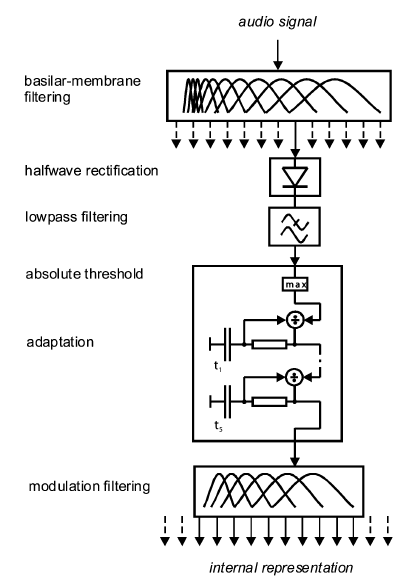
\includegraphics[width = .47\textwidth]{pic/pemoq.png}
    \caption{Blokové schéma modelu sluchové cesty v PEMO-Q\cite{article:pemoq}}
    \label{pic:pemoq}
\end{figure}

Prvním blokem je banka třiceti pěti gammatónových filtrů simulující funkci bazilární membrány. Střední kmitočty jednotlivých filtrů jsou v rozsahu od 235 Hz až po 14,5 kHz. Každá větev je zpracovávána nezávisle. Následné usměrnění a filtrace dolní propustí reprezentuje převod zvuku na nervové impulzy. Zpracovaný signál je přiveden do bloku adaptivní filtrace složeného z pěti zpětnovazebních smyček zapojených do kaskády. Na konci cesty je další banka osmi filtrů modelujících schopnost rozpoznání amplitudově modulovaného zvuku.

\begin{figure}[h]
    \centering
    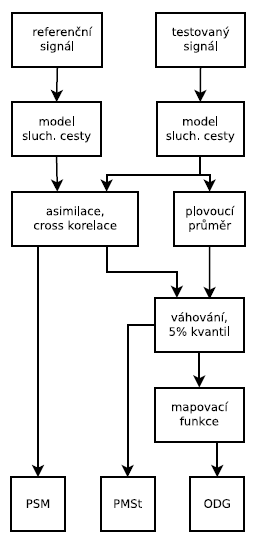
\includegraphics[width = .25\textwidth]{pic/pemoq2.png}
    \caption{Blokové schéma algoritmu PEMO-Q \cite{thesis:zalabak}}
    \label{pic:pemoq2}
\end{figure}

Před kognitivním zpracováním je provedena asimilace signálu. Jedná se o matematický průměr vnitřních tří-dimenzoinálních reprezentací (frekvenční, časové a modulační) testovaného a referenčního signálu tam, kde testovaný nabývá nižších hodnot než signál referenční. Tato operace vychází z poznatku, že \uv{chybějící} prvky jsou méně rušivé než prvky \uv{přidané}. 
Poté je provedena korelace pro každý modulační kanál zvlášť přes všechny časové a frekvenční hodnoty. Z kvadrátů výsledků korelačních funkcí je poté vypočítána hodnota $PSM$ (\textit{Perceptual Similarity Measure}) a z ní i hodnota $ODG$.

\subsection{ViSQOLAudio}

Evolucí původního algoritmu ViSQOL přestaveného v podkapitole \ref{subchapter:visqol} určeného k hodnocení hudebních signálů je tak zvaný ViSQOLAudio. V článku \textit{ViSQOLAudio: An objective audio quality metric for low bitrate codecs} \cite{article:visqolaudio} autoři tvrdí, že k adaptaci původní metody na hodnocení hudebních nahrávek bylo třeba jen drobných změn.

\medskip

Zde je jejich výčet:

\begin{itemize}
    \item Systém porovnávání políček referenčního a testovaného signálu je zachován, nicméně všechna políčka jsou nyní označena za \uv{aktivní} na rozdíl od původních třech signifikantních pro řečové signály.
    \item Množství frekvenčních pásem při předzpracování bylo rozšířeno na celé slyšitelné pásmo od 50 Hz do 20 kHz.
\end{itemize}
%%\chapter{Testovaný materiál}
\label{chap:material}

\epigraph{\hfill\textit{Každá dostatečně rozvinutá technologie je prakticky nerozeznatelná od magie.}}{Arthur C. Clarke}




\chapter{Realizace subjektivních a objektivních testů}
\label{chap:realization}

\epigraph{\textit{\hfill Dvakrát měř, jednou řež.}}{-české přísloví}

K ověření předpokladu, zda objektivní algoritmy hodnotí poslechovou kvalitu nekorektně, k realizaci testů, k přípravě zvukových vzorků a k zobrazení výsledků bylo třeba využít poměrně početného programového vybavení, z jisté části ještě neexistujícího. Vzhledem ke zkušenostem autora s prostředím \matlab z dob bakalářského studia, bylo pro tyto účely využito právě toto interaktivní programové prostředí a skriptovací programovací jazyk čtvrté generace vyvíjený společností MathWorks \cite{web:matlab}. Tato kapitola popisuje jaké existující nástroje byly využity, jak byly propojeny pomocí skriptů napsaných v prostředí \matlab a jaká uživatelská rozhraní byla vytvořena pro uskutečnění poslechových testů a zobrazování výsledků.

\section{Příprava testovaného materiálu}

Před provedením jakýchkoli testů, ať už poslechových či automatizovaných, bylo potřeba připravit množinu zvukových vzorků spolehlivě reprezentující sledované parametry. To znamenalo výběr implementace kodeků, tvorbu skriptů, které je budou dávkově volat a tím generovat vzorky o různých bitových rychlostech a dalších parametrech.

\subsection{Použité kodeky}

U standardů digitálního rádia je struktura jasně definována na vysílací straně a implementace přijímače je ponechána na výrobci zařízení. Ač to může znít paradoxně, u kodeků je tomu právě naopak. Dekodér je normou důkladně popsán, zatímco kodéry mohou být napsány (či sestaveny) různě. Velké společnosti na poli audiovizuálního zpracování, jako například Fraunhoffer či Apple, si licencují vlastní (proprietární) kodéry a nechávají si za ně zaplatit poměrně velké peníze. Proto se souběžně s nimi snaží open-source komunita vytvářet kodéry vlastní. U dvou vzorků stejného profilu a stejné bitové rychlosti se tak může lišit poslechová kvalita, kvůli čemuž je důležité poznamenat jakým kodérem byl signál zakódován.

Na následujících řádcích jsou vyjmenovány implementace kodérů a dekodérů použitých v této práci.
 
\begin{itemize}
    \item TwoLame:
    
použitý ke kódování vzorků do MPEG 1 Layer II je adaptací původního freeware kodéru známého jako tooLame. Je volně dostupný z webových stránek \cite{web:twolame}. Skript \code{makeMp2} volá tento kodér napsaný v jazyce C a generuje vzorky s následujícími parametry:

    \begin{itemize}
        \item konstantní bitová rychlost (kb/s): 56, 64, 80, 96, 112, 128, 160, 192, 224, 256, 320, 384
        \item mód: stereo
        \item vzorkovací rychlost 44100 Hz
    \end{itemize}
    Pro objektivní hodnocení je ovšem nutno mít signál uložený v nezakódované formě. Vzorky tudíž byly převedeny zpět do pulzně kódové modulace pomocí programu FFmpeg \cite{web:ffmpeg}.

    \item Nero AAC Codec
    
    I u rodiny AAC byl v této práci použit freeware nástroj. Nero AAC Codec dostupný z \cite{web:nero} dokáže signál jak kódovat, tak převádět zpět do formy PCM. Dostupné profily jsou: AAC LC, HE-AAC a HE-AAC v2.
    Skript \code{makeAac} volá program \code{NeroAacEnc.exe} a vytváří vzorky s parametery:
        \begin{itemize}
        \item konstantní bitová rychlost : 12 - 256 kb/s pro profil AAC LC, 16 - 128 kb/s pro profil HE-AAC a 12 - 64 kb/s pro profil HE-AAC v2 vždy s krokem 4 kb/s.
        \item mód: stereo (pro HE-AAC v2 mód mono neexistuje, neboť využívá Parametrického sterea)
        \item vzorkovací rychlost 44100 Hz
    \end{itemize}

    \item Opus
    
    \dots je od základu vyvíjen jako open-source. Kodek je proto ke stažení přímo na stránkách standardu \cite{web:opus} a není třeba složitě shánět alternativy ve formě komunitních projektů. Podobně jako u dvou předchozích byl v matlabu vytvořen skript pro generování vzorků s následujícími parametry:
    
    \begin{itemize}
        \item konstantní bitová rychlost : 8 - 128 kb/s s krokem 4 kb/s.
        \item mód: stereo
        \item vzorkovací rychlost 44100 Hz
    \end{itemize}

    \item xHE-AAC
    
    Kódování do xHE-AAC je prozatím problematické neboť jediný současný enkodér poskytuje Fraunhoffer Institute za cenu pro komerční využití. Bylo tak třeba porozhlédnout se po zdroji zakódovaných vzorků jinde.
    Na webu DRM+ \cite{web:drm} je k dispozici ukázkové video v nezkomprimované verzi obsahující tři vzorky jak v originálu, tak zakódované pomocí xHE-AAC do dvou bitových rychlostí. Konkrétně do 8 a 12 kb/s. Pomocí programu Avidemux \cite{web:avidemux} byla z videa extrahována zvuková stopa, ze které byly programem Audacity \cite{web:audacity} vystřihány konkrétní zhruba osmi vteřinové vzorky.
    
\end{itemize}

\subsection{Typy materiálu z hlediska obsahu}
\label{subchap:material}

Doposavad se tato kapitola věnovala tomu, jak hudební vzorky zakódovat a rozkódovat. Neméně důležitým aspektem je ale skutečný obsah nahrávek použitých k testování kvality. Jelikož v éteru rádia existuje mnoho stanic vysílající různý druh obsahu od mluveného slova přes klasickou hudbu až po nezařaditelné alternativní hudební žánry, bylo třeba do palety zpracovávaných vzorků zahrnout různorodý materiál.

Tři vzorky z DRM+ videa představovaly tři kategorie, do kterých jsou nadále rozděleny všechny nahrávky figurující v této práci. Jedná se o signály:

\begin{enumerate}
    \item hudební - v indexech a skriptech značené jako \textit{music}
    \item řečové - s označením \textit{speech}
    \item smíšené - s označením \textit{mixed}
\end{enumerate}

Dalším zdrojem nahrávek byla samotná norma ITU-R BS.1387-1 \cite{itur:1387}, respektive CD přiložené k softwaru Opera \cite{web:opticom} s nahrávkami, které se používají při implementaci algoritmu PEAQ. Jedná se o izolované ukázky různých zvuků či nástrojů jako například klavír, saxofon a zpěv. V rádiu se ovšem takto osamostatněné nástroje vyskytují jen zřídka a proto z nich byl vybrán pouze jeden vzorek, konkrétně úryvek vokální skladby \textit{Tom's Diner} zpěvačky Suzanne Vega, který se ve světě multimediální techniky používá velmi často a může tak fungovat jako určitá reference vůči ostatním testům.
Zbytek nahrávek uvedených v tabulce \ref{table:material} připravil Miroslav Smutný při spolupráci na článku \textit{Perceived Audio Quality Analysis in Digital Audio Broadcasting Plus System Based on PEAQ} \cite{article:ulovecsmutny}.

\begin{table}[h]
    \centering
    \begin{tabular}{|c|c|c|c|}
    \hline
    Název vzorku & Typ & Popis & Zdroj \\ \hline
    'capriccio.wav' & Music & Úryvek klasické hudby & Smutný \\ \hline
    'holmes.wav' & Speech & Čtení z knihy Sherlock Holmes & Smutný \\ \hline
    'cimrman.wav' & Speech & Záznam hry Opeřený Had & Smutný \\ \hline
    'dubstep.wav' & Music & Elektronická hudba & Smutný \\ \hline
    'pennylane.wav' & Music & Úryvek písně od The Beatles & Smutný \\ \hline
    'refveg.wav' & Music (vocal) & A Capella zpěv & Opera \\ \hline
    'frekv3.wav' & Mixed & Řeč s hudebním podkresem & Smutný \\ \hline
    'xhedemomusic.wav' & Music & Hra na elektrickou kytaru & DRM \\ \hline
    'xhedemospeech.wav' & Speech & Úryvek řeči moderátora BBC & DRM \\ \hline
    'xhedemomixed.wav' & Mixed & Řeč s hudebním podkresem & DRM \\ \hline
    \end{tabular}
    \caption{Seznam vzorků použitých při objektivním testování kvality}
    \label{table:material}
\end{table}

Hlavně pro potřeby subjektivního testování byly za pomoci programu Audacity z nahrávek vybrány relevantní desetivteřinové úseky, které byly dále opatřeny pozvolným zesílením v první vteřině a pozvolným útlumem ve vteřině poslední.

\section{Návrh subjektivních testů}

Jak už je v úvodu naznačeno, objektivní hodnocení nahrávek zakódovaných novými kodeky využívajícími psychoakustické poznatky ve vetší míře nekoresponduje s realitou. Na tento fakt již poukazuje akademický článek \textit{Subjective and Objective Assessment of Perceived AudioQuality of Current Digital Audio Broadcasting Systems and Web-Casting Applications.} \cite{article:pocta}, kde je sledována závislost $ODG$ a $SDG$ při použití hodnotících algoritmů PEAQ a POLQA. Subjektivní testy provádí párovým srovnáváním podle \cite{itur:1116}, tedy na velké skupině expertních posluchačů. Pro potřeby této práce se ovšem lépe hodí test s vícenásobným stimulem dle \cite{itur:1534}

\subsection{Důvody pro výběr testu MUSHRA}
\begin{itemize}
    \item Zkoumaná kvalitativní oblast
    
    Protože bylo třeba ověřit zda algoritmy hodnotí věrohodně nejen tam kde je komprese nepostřehnutelná, ale skrze celé kvalitativní spektrum od výborné až po nedostatečnou, je test pro střední kvalitu podle \cite{itur:1534} mnohem vhodnější než test pro nepatrná zhoršení použitý v \cite{article:pocta}. Největší důraz bylo třeba klást na bitové rychlosti využívané v digitálním rádiu DAB/DAB+ a DRM.
    
    \item Posluchači

    Subjekty nemusí procházet sérií rozřazovacích vstupních testů. Stačí pouze zaučení přímo v grafickém uživatelském rozhraní samotného testu a doprovodné informace v přiloženém návodu (K nahlédnutí v příloze \ref{app:2}).
    
    \item Podmínky
    
    MUSHRA nemá tak přísné podmínky na provádění testu. K jeho provedení není třeba poslechová místnost s extrémně kvalitním reprodukčním zařízením. Stačí dostatečně kvalitní sluchátka a úroveň zvukového pozadí taková, aby nerušila posluchače.
    Další výhodou tohoto testu je, že lze provádět individuálně. Je tedy možné přenášet laptop se zvukovou kartou a sluchátky za subjekty a tím ušetřit čas i náklady.
\end{itemize}

\subsection{Výběr vzorků}

Jednou z nesporných výhod objektivního testování je absence únavy posluchačů, se kterou je třeba počítat při návrhu subjektivního testu. Doporučení \cite{itur:1534} říká, že délka testu by neměla překročit půl hodiny. Přímo naproti tomu jde fakt, že k zachování objektivity je třeba dostatečná diverzita poslechového materiálu. Výběr těch správných vzorků se tak stává poměrně zásadním faktorem pro výpovědní hodnotu navrženého testu.

Jak už je zmíněno v podkapitole \ref{subchap:material}. Vzorky byly rozděleny do třech kategorií. Hudební, řečové a smíšené. V druhých dvou zmíněných nedosahuje míra různorodosti vzorků takové výše jako v kategorii hudební. Vetší důraz byl tedy kladen právě na ni, a proto je v subjektivním testování zahrnuto několik vzorků reprezentujících různé hudební žánry.

Stimuly musí být, co do metody zkreslení, konzistentní skrze všechny zkoušky testu a nemožnost kódování nových zvukových záznamů do xHE-AAC tak značně zkomplikovala přípravu vzorků. Nakonec byly vytvořeny testy dva. Jeden na vyšších bitových rychlostech, obsahující všechny kodeky vyjma xHE-AAC. A druhý test na nižších datových tocích, kde společně s xHE-AAC vystupovaly zástupci novodobých kódovacích metod.

Zkoušky sestavených testů tedy obsahují vzorky uvedené v tabulce \ref{table:material:subjective}.

\begin{table}[h]
    \centering
    \begin{tabular}{|c|c|c|c|}
    \hline
    Název vzorku & Typ & Popis & Test \\ \hline
    'capriccio.wav' & Music & Úryvek klasické hudby & 1 \\ \hline
    'holmes.wav' & Speech & Čtení z knihy Sherlock Holmes & 1 \\ \hline
    %'cimrman.wav' & Speech & Záznam hry Opeřený Had & Smutný \\ \hline
    %'dubstep.wav' & Music & Elektronická hudba & Smutný \\ \hline
    'pennylane.wav' & Music & Úryvek písně od The Beatles & 1 \\ \hline
    'refveg.wav' & Music (vocal) & A Capella zpěv & 1 \\ \hline
    %'frekv3.wav' & Mixed & Řeč s hudebním podkresem & Smutný \\ \hline
    'xhedemomusic.wav' & Music & Hra na elektrickou kytaru & 2 \\ \hline
    'xhedemospeech.wav' & Speech & Úryvek řeči moderátora BBC & 2 \\ \hline
    'xhedemomixed.wav' & Mixed & Řeč s hudebním podkresem & 1,2 \\ \hline
    \end{tabular}
    \caption{Seznam vzorků použitých v subjektivních testech}
    \label{table:material:subjective}
\end{table}

\begin{table}[h]
    \centering
    \begin{tabular}{|c|C{1cm}|C{1cm}|C{1cm}|C{1cm}|C{1cm}|C{1cm}|}
    \hline
    bitrate (kpbs) & 24 & 32 & 48 & 64 & 96 & 128\\
    \hline
    Opus & \cellcolor{green!50} $\bullet$ &$\bullet$ & & & & \\
    \hline
    HE-AAC v2 & &$\bullet$&\cellcolor{green!50}$\bullet$& & &  \\
     \hline
    HE-AAC v1 & & &$\bullet$ &$\bullet$ &  &  \\
     \hline
     LC-AAC & & & & $\bullet$ & & \\
      \hline
     MPEG1 Layer II  & & & & &  $\bullet$ & $\bullet$ \\
       \hline
    \end{tabular}
    \caption{Použité bitové rychlosti v testu č. 1}
    \label{table:test1}
\end{table}

\begin{table}[h]
    \centering
    \begin{tabular}{|c|C{1cm}|C{1cm}|C{1cm}|C{1cm}|C{1cm}|}
    \hline
    bitrate (kpbs) & 8 & 12 & 24 & 48 & 64 \\
    \hline
    xHE-AAC &$\bullet$ &$\bullet$ & & & \\
    \hline
    Opus & & $\bullet$&\cellcolor{green!50}$\bullet$&  &   \\
     \hline
    HE-AAC v2 & & &$\bullet$ &\cellcolor{green!50}$\bullet$ & $\bullet$ \\
     \hline
    \end{tabular}
    \caption{Použité bitové rychlosti v testu č. 2}
    \label{table:test2}
\end{table}
Konkrétní bitové rychlosti použité v testech 1 a 2 jsou zobrazené v tabulkách \ref{table:test1} a \ref{table:test2}. Konečná volba proběhla na základě následujících kriterií: 

\begin{itemize}
    \item Bitové rychlosti používané v digitálním rádiu: 
    
    Například \textit{Advanced Audio Coding} se v systémech digitálního rádia na území České Republiky \cite{web:dab:stations} nachází ve verzích HE-AAC v1 a HE-AAC v2, tedy v základní verzi obohacené o SBR potažmo o PS. V zahraničí lze nalézt multiplexy v nichž se vysílá AAC LC profilem avšak není jich mnoho. Velký důraz je tak kladen na HE-AAC v2 profil. O něco menší na HE-AAC v1 a Low Complexity je zastoupen v testech jen jednou.
    
    \item Oblasti kde se výsledky různých algoritmů rozcházely v předběžných testech: 
    
    Například MPEG Layer II byl v předběžných testech hodnocen různými algoritmy s velkými kvalitativními rozestupy. Vzorky zkomprimované do \textit{mp2} se proto v testu nachází ve dvou bitových rychlostech.
   
    \item Výběr stejných bitových rychlostí různých kodeků k porovnání jednotlivých kompresních metod: 
    
    Kupříkladu k určení toho, jak moc velký vliv mají rozšíření SBR a PS na výslednou kvalitu.
    
    \item Sledování spíše nižších rychlostí pro určení hranice nedostatečné poslechové kvality.
    
\end{itemize}

Zeleně jsou zvýrazněny vzorky, ve kterých se testy vzájemně překrývají.

%\begin{comment}
\subsection{Použité vybavení}

Provést subjektivní testy v poslechové místnosti velkou skupinou posluchačů se ukázalo jako časově a hlavně koordinačně velmi náročné. Byla proto zvolena varianta testu přenosného, který lze realizovat kdykoliv a kdekoliv, kde není přítomno zvukové rušení. Testy byly spouštěny přímo v prostředí \matlab bežícím na čtrnácti palcovém notebooku ThinkPad E431. Jako poslechové zařízení byla použita studiová sluchátka, používaná na katedře Radioelektroniky fakulty Elektrotechnické ČVUT k poslechovým testům v rámci výuky zvukové techniky. Konkrétně šlo o model Sennheisser HD 200 PRO. Parametry udávané výrobcem jsou v tabulce \ref{table:hd200}. 

\begin{table}[h]
    \centering
    \begin{tabular}{|c|c|}
    \hline
    Harmonické zkreslení (THD): & \textless{}0,1 \% \\ \hline
    Jmenovitá impedance: & 32 Ohm \\ \hline
    Délka kabelu: & 2 m \\ \hline
    Frekvenční rozsah: & 20 - 20 000 Hz \\ \hline
    Hmotnost: & 184 g \\ \hline
    Konstrukce: & uzavřená, dynamická \\ \hline
    Akustický tlak: & 108 dB ( 1 Vrms ) \\ \hline
    \end{tabular}
    \caption{Parametry  sluchátek Sennhesier HD 200 PRO udávané výrobcem \cite{web:senn}}
    \label{table:hd200}
\end{table}

Zda frekvenční charakteristika sluchátek odpovídá přísné toleranční masce podle ITU-R BS.708 \cite{itur:708} bylo ověřeno měřením na umělém uchu Brüel \& Kjær 4153 \cite{web:earsim}. Blokové schéma zapojení se nachází na obrázku \ref{pic:measure}.

\begin{figure}[h]
    \centering
    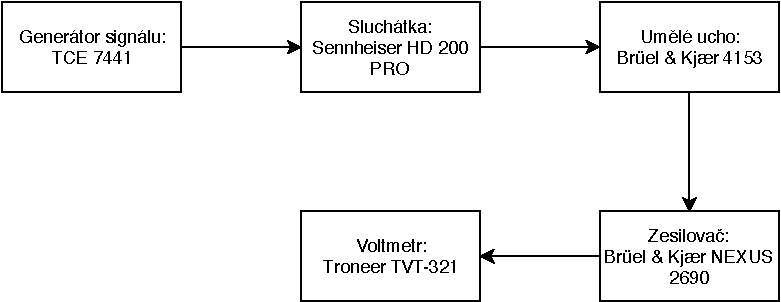
\includegraphics[width = .8\textwidth]{pic/measure.pdf}
    \caption{Blokové schéma zapojení měřícího pracoviště při měření sluchátek Sennhesier HD 200 PRO}
    \label{pic:measure}
\end{figure}

 Naměřená frekvenční charakteristika je na obrázku \ref{pic:hd200}. V nejvyšší části basového pásma a nejnižší oblasti středních kmitočtů nesplňuje přísné hranice masky ITU-R. Sluchátka nicméně byla použita s přihlédnutím k následujícím kritériím.
 
 \begin{itemize}
     \item Doporučení ITU-R BS.1534 MUSHRA se na kvalitu sluchátek odvolávají skrze normu ITU-R BS.1116 pro měření nepatrných zhoršení. Testování v rámci této práce se však zabývá střední kvalitou. 
     \item Frekvenční charakteristika sluchátek Sennheiser HD 280 PRO, která podle webové stránky rtings.com \cite{web:rtings}, věnující se podrobnému měření studiových sluchátek, dosahuje velmi podobného zvlnění a vybočuje tak z masky dané doporučením BS.708 stejně jako Sennheiser HD 200 PRO. I přes to jsou sluchátka HD 280 PRO použita v následujících akademických pracích, které taktéž k hodnocení kvality využívají test MUSHRA.
     \begin{itemize}
         \item \textit{Considering Bluetooth's Subband Codec (SBC) for Wideband Speech and Audio on the Internet} \cite{headphones1} - článek nalezený na webu \textit{Researchgate.com} zabývající se problematikou kódování širokopásmového zvuku pro přenos internetovým rádiem.
         \item \textit{Acoustic echo reduction robust against echo-path change with instant echo-power-level adjustment} \cite{headphones2} - článek nalezený na webu \textit{ieeexplore.com} který se zabývá odstraňováním dozvuku v telekomunikacích.
     \end{itemize}
 \end{itemize}

\begin{figure}[h]
    \centering
    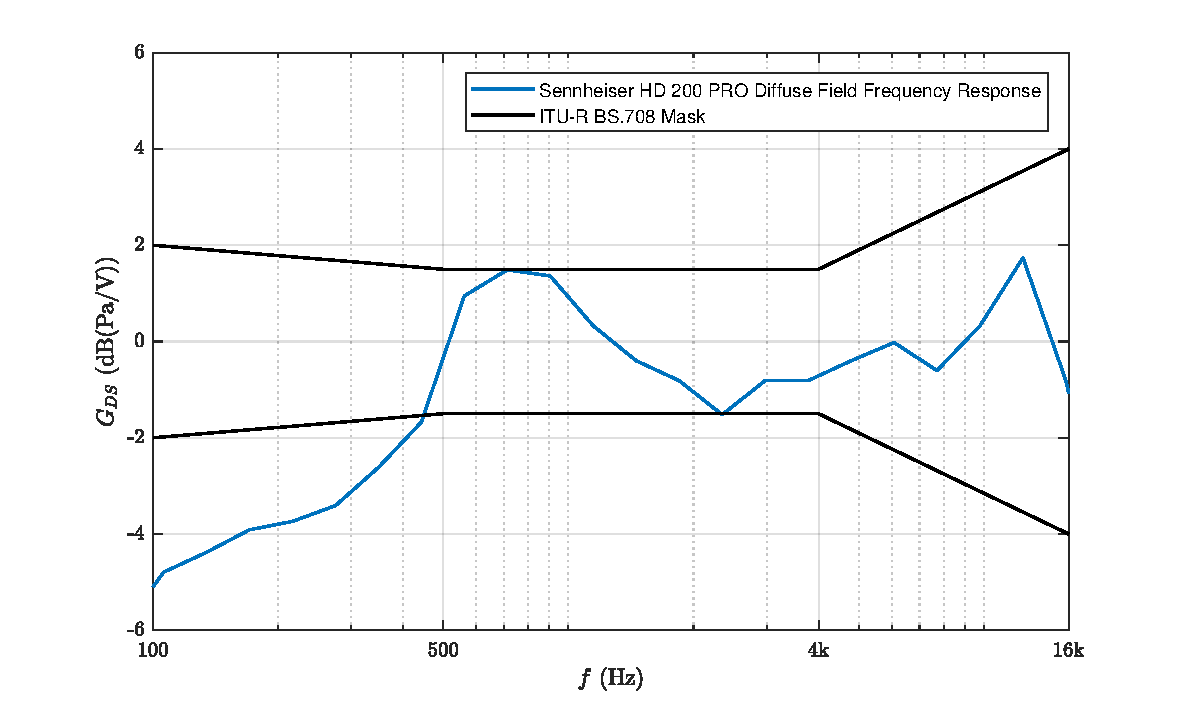
\includegraphics[width = \textwidth]{pic/headphones.pdf}
    \caption{Frekvenční charakteristika sluchátek Sennhesier HD 200 PRO změřená na umělém uchu Brüel \& Kjær}
    \label{pic:hd200}
\end{figure}


K převodu na analogový signál byla použita externí zvuková karta AxagonHQ ADA-HP, jejíž relevantní technické parametry udávané výrobcem jsou uvedeny v tabulce \ref{table:soundcard}. Hladina okolního šumu nebyla při provádění testu měřena, nicméně byl kladen důraz na to, aby ruch okolí nerušil subjekty při poslechu.

\begin{table}[h]
    \centering
    \begin{tabular}{|c|c|}
    \hline
    Analogový výstup & \begin{tabular}[c]{@{}c@{}}2kanálový stereo výstup pro sluchátka \\ nebo aktivní reproduktory\end{tabular} \\ \hline
    Vzorkovací frekvence & 44.1 / 48 / 96 kHz analog \\ \hline
    Rozlišení & 16 / 24 bit pro přehrávání \\ \hline
    Odstup signál / šum & $\geq$ 95dB (Output SNR) pro DAC \\ \hline
    Harmonické zkreslení & $\leq$ -85dB (Output THD+N) \\ \hline
%    Konektor & 3.5 mm stereo jack (sluchátkový výstup) \\ \hline
%    Rozhraní & USB 2.0 / USB 1.1 \\ \hline
    \multicolumn{1}{|l|}{Sluchátkový zesilovač} & \multicolumn{1}{l|}{\begin{tabular}[c]{@{}l@{}}20 - 20.000 Hz, výkon 105 mW / 16 ohm,\\  při 1kHz 0.1\% THD+N, 16 - 100 $\Omega$\end{tabular}} \\ \hline
    \end{tabular}
    \caption{Parametry zvukové karty AxagonHQ ADA-HP udávané výrobcem \cite{web:axagon}}
    \label{table:soundcard}
\end{table}

\subsection{Grafické uživatelské rozhraní}

Jelikož MUSHRA test se využívá k poslechovým testům více než deset let, existují již před-připravené skripty a programy do kterých stačí naimportovat vzorky a není třeba se zabývat programováním GUI a vyhodnocovacích algoritmů. Většina takových programů je ovšem zatížena licenčními polatky. Vedle komerčních produktů existují i komunitou psané freeware programy jako jsou WhisPER\cite{article:whisPER}, APE\cite{article:APE} a Scale. 

Po zvážení byl vybrán právě program Scale \cite{article:scale} připravený pro použití v jazyce \matlab. Jeho předností by měla být implementace rozhraní pro provádění všech testů popsaných v kapitole \ref{chap.listeningTests}. Kromě samotného testu se pyšní i schopností výsledky vyhodnotit.

Po několika pokusech využít Scale se ovšem začaly objevovat problémy. Při větším množství vzorků nahraných do rozhraní MUSHRA prostředí \matlab hlásilo chyby, vyhodnocování bylo spolehlivé pouze pro test pro nepatrná zhoršení \cite{itur:1116} a jednodušší než opravovat existující program se začalo zdát napsat si program od základu.

%\subsection{Zvolené prostředí}

Pro návrh grafického uživatelského rozhraní se v matlabu nachází komponenta GUIDE \cite{web:guide}. Jedná se o nástroj, ve kterém se pomocí kurzoru myši dají rozmístit objekty z nabídky do prostoru okna, které se poté oživují psaním funkcí zvaných \textit{callbacks}. Ty jsou vyvolány akcemi jako například kliknutím myši, či stiskem klávesy. Objekty jsou definovány souborem vlastností uložených ve speciálním datovém typu \textit{handle} a jdou dle potřeby vyčítat či upravovat obdobně jako standardní datové proměnné v klasických funkcích. Na následujících řádcích je stručně popsáno výsledné rozhraní, ve kterém byly testy MUSHRA realizovány.

\begin{itemize}
    \item Uvítací okno
    
    Jednoduché GUI s rámcovým popisem testu, dvěma dialogy pro zadání jména a věku subjektu a tlačítkem pro přechod do další fáze testu. Uvítací okno je k vidění na obrázku \ref{pic:intro}.
    
    \begin{figure}[h]
        \centering
        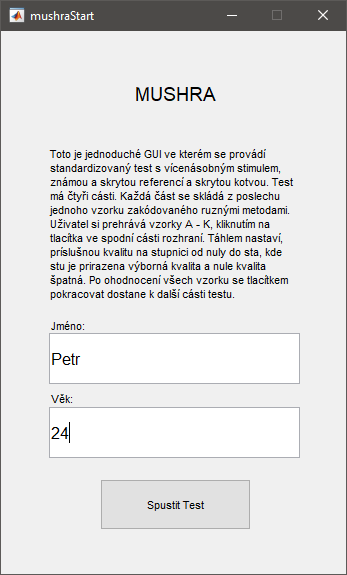
\includegraphics[width=.32\textwidth]{pic/intro.png}
        \caption{Grafické rozhraní uvítacího okna}
        \label{pic:intro}
        \end{figure}
        
        \item Zaučení
        
        Okno velmi podobné \uv{ostrému} testování. Na rozdíl od něj zde nejsou vzorky seřazeny náhodně, ale pod každým tlačítkem se nachází zvuková nahrávka odpovídající popisu v pravé části okna. Uživatel si takto může jednotlivé typy stimulů projít a naučit se, co je to \uv{kotva}, \uv{skrytá reference} a na jaké druhy zkreslení může při testu narazit.

\begin{comment}
    \begin{figure}[h]
    \centering
    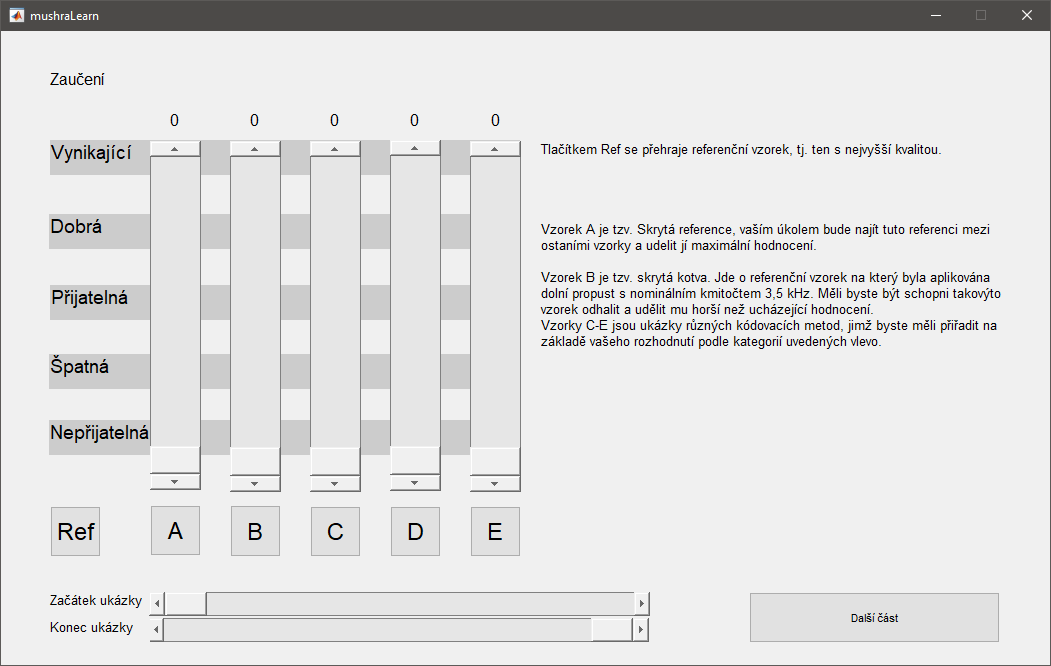
\includegraphics[width=.75\textwidth]{pic/learn.png}
    \caption{Grafické rozhraní části zvané: Zaučení}
    \label{pic:learn}
    \end{figure}
\end{comment}    

    \item Okno pro jednu zkoušku testu
    
    
Toto okno se přizpůsobuje na základě toho jaký návrhář testu zvolí počet zkoušek a vzorků. Soubor \code{scenarios.txt} v kořenovém adresáři testu, obsahuje názvy jednotlivých zkoušek oddělených novým řádkem. Pro představu test popsaný v tabulce \ref{table:test1} je zapsán takto:

\samepage{\code{Klasická hudba\\
Rock\\                            
Mluvené slovo\\
Zpěv(acapella)\\
Mixed}}

Tomu musí odpovídat počet podsložek uložených do složky \code{scenarios}. Podle počtu vzorků v podsložkách se aktivuje počet přehrávacích tlačítek hodnotících posuvníků. Maximálně jich ovšem může být 12 včetně dvou referencí a jedné kotvy.

Nad každým posuvníkem se nachází udělené hodnocení v procentech. Pro lepší orientaci jsou posuvníky podkresleny barevně odlišenými oblastmi, které odpovídají kvalitativním úrovním definovaným v doporučení ITU-R BS 1534.

Po vyplnění všech zkoušek je test ukončen dialogovým oknem s nápisem \uv{Konec!}, které volá funkci pro export výsledků do souboru.

O průměrování, post-screening a zobrazení do sloupcových grafů se stará skript \code{displayResults}, taktéž umístěný v kořenovém adresáři testu.

\begin{figure}[h]
\centering
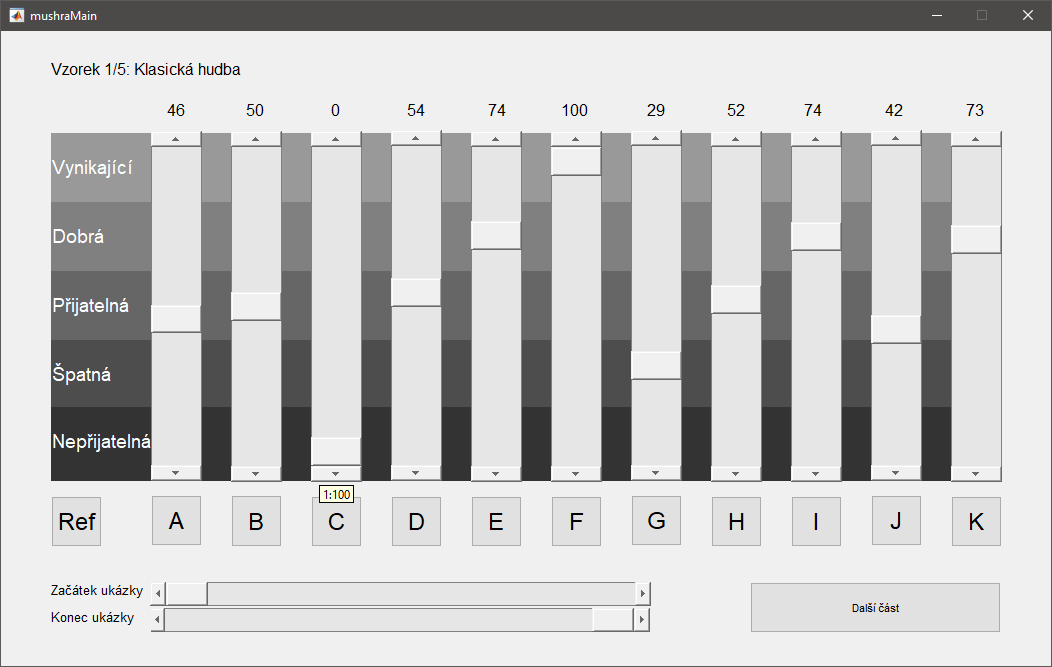
\includegraphics[width=.95\textwidth]{pic/test.png}
\caption{Grafické rozhraní průběhu testu}
\label{pic:test}
\end{figure}

Posuvníky ve spodní části okna nazvané \uv{Začátek ukázky} a \uv{Konec ukázky} slouží k časovému omezení všech přehrávaných vzorků dané zkoušky. Touto funkci lze využít při rozhodování pouze na základě krátkého úseku vzorku. Například při podezření, že se v ukázce vyskytuje kompresní artefakt.


\end{itemize}

\section{Použité implementace algoritmů pro objektivní testování kvality audiosignálů}

\subsection{PEAQ}

Matlabová implementace PQevalAudio základního modelu PEAQ je volně k dispozici na stránkách univerzity McGill \cite{web:mcgill}. V předběžných testech byl využit právě tento model, nicméně sami autoři v poznámkách tvrdí, že slouží pro výukové účely a nikoliv pro výzkum na poli zvukového zpracování, jelikož nesplňuje všechna kritéria vytyčená doporučením \cite{itur:1387}. Proto se v praxi se základní verzí algoritmu příliš nesetkáváme. Pokročilá verze byla implementována v roce 2003 do programu s názvem Opera\footnote{Opera obsahuje i základní verzi algoritmu PEAQ.} německou firmou OPTICOM \cite{web:opticom}, která se soustředí na vývoj softwaru pro hodnocení kvality zvuku již od roku 1995 a podílela se i na vzniku standardu \cite{itur:1387}. Katedra radiotechniky ČVUT má zakoupenou licenci tohoto programu pro akademické využití. K ověření platnosti licence využívá USB klíčenku, kterou je třeba mít připojenou k PC po celou dobu běhu algoritmu.

Rozhraní programu (na obrázku \ref{pic:Opera}) je poměrně spartánské. V levém horním rohu se nachází tlačítka pro obsluhu. Zbytek prostoru je vyhrazen pro prezentaci výsledků hodnocení. Tlačítkem \uv{Start} s obrázkem vlaječky se spouští průvodce importem vzorků. Lze použít různé mapování kanálů, kompenzaci zpoždění, a několik filtrů, například odstranění stejnosměrné složky.

Po zadání všech parametrů a cest k referenčnímu a testovanému vzorku přejde program k hodnocení a po dokončení běhu algoritmu zobrazí výsledky jako například: zpozdění, rozdíl hlasitostí vyjádřený v úrovních, délky vzorků a především $ODG$ s grafickou reprezentací.

\begin{figure}[h]
    \centering
    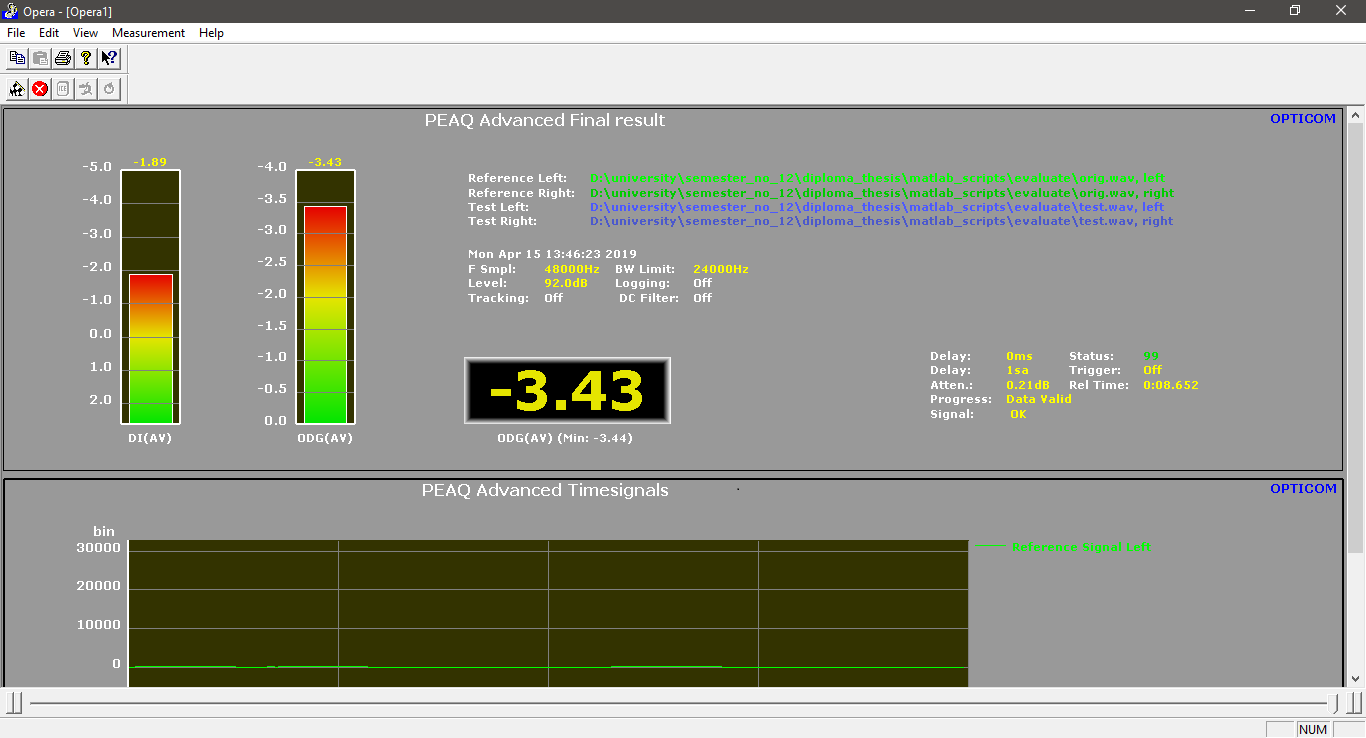
\includegraphics[width=.95\textwidth]{pic/opera.png}
    \caption{Uživatelské rozhraní programu OPERA}
    \label{pic:Opera}
\end{figure}


Takovýto postup je časově náročný a při hodnocení stovek až tisíců vzorků nepoužitelný. Naštěstí lze Opera volat z příkazové řádky a tím je proces automatizovatelný. Volání programu \code{opera.exe} vrací záznam ve formě tabulky v textovém souboru, ze kterého lze parametry předat jiným programům.

I přes to, že se v akademické sféře používá pokročilý model, čistě ze zvědavosti autora jsou v této práci zahrnuty výstupy obou verzí algoritmu počítané programem Opera.

\subsection{PEMO-Q}

Balík \code{OpenQual+} vznikl jako přepis implementace algoritmu PEMO-Q z diplomové práce Martina Zalabáka \cite{thesis:zalabak} užitím principů objektově orientovaného programování. Zároveň je kód upravený tak, aby poskytoval výsledky blížící se verifikované komerční implementaci PEMO-Q od HörTech gGmbH \cite{web:hortech}. Jeho autor Jan Novák ve své bakalářské práci \cite{thesis:novak} zmiňuje, že balík je optimalizovaný pro \matlab 2017a a novější. Ve verzi 2018b nicméně vykazoval značně podivné chování často končící chybou, což je důvod proč je v této práci použito právě prostředí 2017a i přes svou téměř dvou roční zastaralost. Smyslem objektově orientovaného přístupu při programování \code{OpenQual+} byla myšlenka jednoduché rozšířitelnosti o další hodnotící algoritmy. V této práci je ovšem využita pouze pro hodnocení metodou PEMO-Q.

Inicializace balíku probíhá skrze metodu \code{ getEvaluationEngine}, která po zadání parametrů vrátí instanci třídy modelu, se kterým se dá následně pracovat jako s obyčejnou funkcí pomocí příkazu \code{ engineInstance.evalObjQuality(y,y1)}, kde \code{y} je referenční vzorek a \code{y1} je vzorek testovaný.
Ve srovnání s programem Opera je hodnocení poměrně časově náročné.

\subsection{ViSQOL Audio}

Zprovoznění implementace algoritmu ViSQOL bylo ze všech použitých implementací nejjednodušší. Jedná se o funkci \code{visqol.m} napsanou v jazyce \matlab dostupnou z \cite{web:visqol} se vstupy pro referenční signál, testovaný signál a parametry. Těmi je konkrétně myšleno, zda bude použit základní model pro hodnocení hlasu či pokročilý ViSQOL-Audio.

Jelikož původně byl algoritmus ViSQOL vyvíjen k hodnocení kvality přenosu řeči v telekomunikacích, neposkytuje výsledky ve formě $ODG$, ale na škále \textit{MOS-LQO} (\textit{Mean Opinion Score - Linear Quadrature Objective}). Je to taktéž jediný výstup funkce \code{visqol.m}, což může být bráno jako nevýhoda oproti algoritmům PEAQ a PEMO-Q, které disponují větším množstvím výstupních parametrů.
\begin{comment}
    V doporučení \cite{itur:1284} v kapitole 5: \textit{Grading Scales}, je tabulka (uvedená na obrázku \ref{pic:mosodg}), která pokládá pomyslné rovnítko mezi stupnice \textit{MOS} a $ODG$. 
    
    \begin{figure}[h]
        \centering
        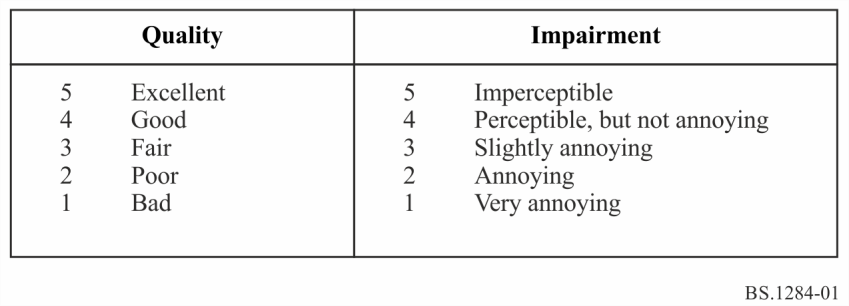
\includegraphics[width=0.7\textwidth]{pic/mos_odg.png}
        \caption{Vztah $MOS$ a $SDG$ ($ODG$) z \cite{itur:1284}}
        \label{pic:mosodg}
    \end{figure}
\end{comment}


\section{Popis ostatních funkcí, skriptů a rozhraní}

V průběhu této diplomové práce bylo připraveno v rozhraní \matlab několik skriptů, funkcí a programů, jenž slouží ke generování vzorků, jejich hodnocení a zobrazování výsledků. V následujících podkapitolách je popsána jejich funkce a ovládání.

\subsection{main}

Main je skript propojující většinu funkcí, skriptů a podprogramů, použitých při vyhodnocování kvality zvuku. Jeho kompletní kód je v digitální příloze.% \ref{code:main}.
Postupně se na základě uživatelského vstupu stará o:
\begin{itemize}
    \item inicializaci cest
    \item přípravu zakódovaných souborů
    \item hodnocení objektivními algoritmy
    \item zobrazení výsledků
\end{itemize}

\subsection{evaluate}

Funkce \code{evaluate} provádí sekvenčně několik operací. Na základě vybraného kodeku přidělí možné bitové rychlosti, ve kterých je hodnocení možné. Následně načte testovaný vzorek, k němu ve složce \code{original} vyhledá referenci a vyřeší časové zarovnání, bez něhož by hodnocení nebylo korektní. Poté oba vzorky předá hodnotícímu algoritmu, popřípadě provede převzorkování na jiný kmitočet, a výsledné hodnocení uloží do souboru pro další zpracování.

\subsection{showResults}

Grafické rozhraní \code{showResuls} slouží k prezentaci závislostí $ODG$ na bitové rychlosti, získaných z výstupů objektivních algoritmů pomocí funkce \code{evaluate}. K návrhu byl využit systém GUIDE \cite{web:guide}. Okno programu na obrázku \ref{pic:showResults} je rozdělené do dvou částí. Vlevo se nachází ovládací prvky, vpravo je prostor pro zobrazení grafů. Vykreslení grafů reaguje okamžitě na uživatelem volenou kombinaci kodeků (přepínačem \textit{Codec}) a hodnotící metody (přepínačem \textit{Method}). Tlačítkem \textit{Choose Samples} se otevře dialogové okno \code{ChooseDialog}, ve kterém je možné vybrat si pouze vzorky, jenž uživatele zajímají. Přepínačem \textit{Display} lze vykreslit celou množinu závislostí, či jejich aritmetický průměr společně se směrodatnou odchylkou.
Hodnoty na ose \textit{x} lze buďto nechat automaticky se přizpůsobovat obsahu grafu, nebo lze zatrhávacím boxem \textit{Fixed Bitrate} zvolit pevný rozsah v intervalu $\langle12;384\rangle$ kb/s.

\begin{figure}[h]
\centering
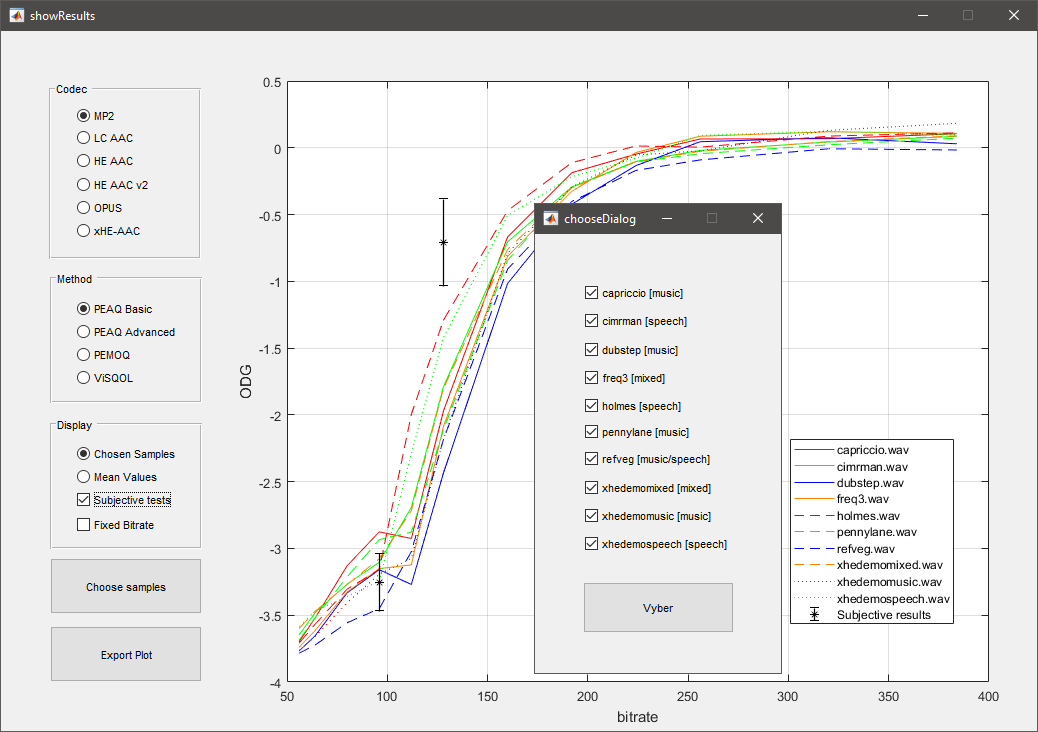
\includegraphics[width=.85\textwidth]{pic/showResults.png}
\caption{Grafické rozhraní \code{showResults}}
\label{pic:showResults}
\end{figure}

Zatrhávací box \textit{Subjective tests} umožňuje zobrazit výsledky subjektivních testů, pokud jsou k dispozici. Protože rozhraní \code{showResults} bylo vymyšleno pro vykreslování výsledků hodnocení objektivními algoritmy, je tato funkce pouze doplňková a nectí set vybraných vzorků tlačítkem \textit{Choose Samples}, který ostatně vůbec nemusí být shodný.  Při kliknutí myší na tento box se zobrazí varování o tom, na kterých vzorcích byl subjektivní test proveden. Je ponecháno na uživateli, aby dbal na to jaká data porovnává. 
Grafy lze exportovat tlačítkem \textit{Export Plot} do formátů pdf, png, jpeg a bmp..

\subsection{makeCell}

Výsledky objektivního hodnocení je do zobrazovače \code{showResults} třeba importovat. Skript \code{makeCell} je jednoduchý kód jehož úkolem je kumulace výsledků (závislostí $ODG$ na bitových tocích) z funkce \code{evaluate} do jednoho souboru, se kterým se bude lépe pracovat. V Matlabu pro takové aplikace existuje datový typ zvaný buňka (\textit{cell}), do kterého jdou nořit libovolné datové typy. Buňka
vytvořená pomocí funkce \code{makeCell} má následující kořenovou strukturu:

\centerline{\code{cellName/algorithms/codecs/odgs}}


%%\chapter{Objektivní testování}
\label{chap:objetiveTests}

\chapter{Výsledky testů}
\label{chap:results}

\section{Výsledky subjektivních testů}

Nakonec byly oba testy představené v kapitole \ref{chap:realization} provedeny sedmnácti subjekty ve věkovém intervalu od 21 do 62 let. Šest z nich mělo předchozí zkušenosti s poslechovými testy. Poměr mužských posluchačů vůči ženám byl přibližně 2:1. Všem byly poskytnuty průvodní informace, prošli fází zaučení a podepsali informovaný souhlas. 

Dvě formy post-screeningu byly aplikovány na množinu získaných hodnocení. První za pomoci skryté reference a druhá pomocí skryté kotvy. Doporučení říká, že subjekty jejichž hodnocení skryté reference je v patnácti procentech případů nižší než devadesát procent, by měli být vyřazeni. To je poměrně přísná podmínka a při jejím aplikování by bylo vyřazeno více než 60 \% subjektů. Protože test míří na běžné posluchače rozhlasového vysílání, nikoliv na studiový poslech znalými posluchači, bylo toto kritérium poníženo a vyřazeni byli ti, jejichž průměrné hodnocení vzorků bylo nižší než 90 \%. Zároveň nejsou zahrnuta hodnocení posluchačů, jejichž průměrné hodnocení skryté kotvy bylo vyšší než 50 \%. Prvním kritériem byly vyřazeni tři posluchači a druhým jeden další. Celkový počet subjektů s relevantním hodnocením byl tedy roven $N = 12$.

Výsledky poslechových testů jsou vyneseny do tabulek \ref{table:mos:test1} a \ref{table:mos:test2}. Zároveň jsou vyobrazeny pomocí sloupcových grafů, které ukazují průměr subjektivně vnímané poslechové kvality $\overline{u}_{jk}$. Na obrázcích \ref{pic:mushra1} a \ref{pic:mushra2} lze vidět průměrné hodnocení přes všechny zkoušky. Grafy \ref{pic:mushra1:kat} a \ref{pic:mushra2:kat} tyto hodnoty dělí do třech sledovaných kategorií: hudební, řečové a smíšené. Všechny výsledky jsou doplněny chybovými úsečkami vyznačující interval spolehlivosti o velikosti $2\delta_k$ vypočítaný podle vztahu \ref{equation:inteval}, ve kterém se s 95\% pravděpodobností nachází populační průměr. 

\begin{table}[h]
\centering
\begin{tabular}{|c|c|c|c|c|c|c|c|c|c|c|c|}
\hline
 & \rot{128 MP2} & \rot{24 opus} & \rot{32 HE-AAC v2} & \rot{32 opus} & \rot{48 HE-AAC v1} & \rot{48 HE-AAC v2 } & \rot{64 HE-AAC v1} & \rot{64 LC-AAC} & \rot{96 MP2} & \rot{hidden ref} & \rot{lp35}\\ \hline
$\overline{u}_{k}$ & 82,3 & 59,4 & 26,6 & 67,3 & 58,1 & 62,6 & 85,0 & 86,4 & 18,7 & 96,6 & 11,9 \\ \hline
$\delta_{k}$ & 8,1 & 6,9 & 3,7 & 6,7 & 8,5 & 7,5 & 9,0 & 8,4 & 5,4 & 1,9 & 6,8 \\ \hline
$\overline{u}_{jk(music)}$ & 78,2 & 42,2 & 19,7 & 60,0 & 51,1 & 54,7 & 84,8 & 85,6 & 13,3 & 96,8 & 11,5 \\ \hline
$\delta_{jk(music)}$ & 9,0 & 7,2 & 3,2 & 5,2 & 7,2 & 10,0 & 9,8 & 9,4 & 5,7 & 1,6 & 7,6 \\ \hline
$\overline{u}_{k(speech)}$ & 89,0 & 86,7 & 45,8 & 73,5 & 72,4 & 80,1 & 97,0 & 95,4 & 34,3 & 95,9 & 14,3 \\ \hline
$\delta_{k(speech)}$ & 10,5 & 7,0 & 11,7 & 10,9 & 16,2 & 8,8 & 3,1 & 4,5 & 14,1 & 4,3 & 11,4 \\ \hline
$\overline{u}_{k(mixed)}$ & 88,0 & 84,0 & 28,0 & 83,0 & 64,7 & 68,8 & 73,4 & 80,1 & 19,4 & 96,7 & 10,4 \\ \hline
$\delta_{k(mixed)}$ & 6,5 & 9,1 & 7,6 & 12,4 & 11,6 & 10,7 & 19,6 & 16,6 & 10,2 & 2,4 & 9,5 \\ \hline
\end{tabular}
\caption{Výsledky prvního testu}
\label{table:mos:test1}
\end{table}

\begin{figure}[h!]
    \centering
    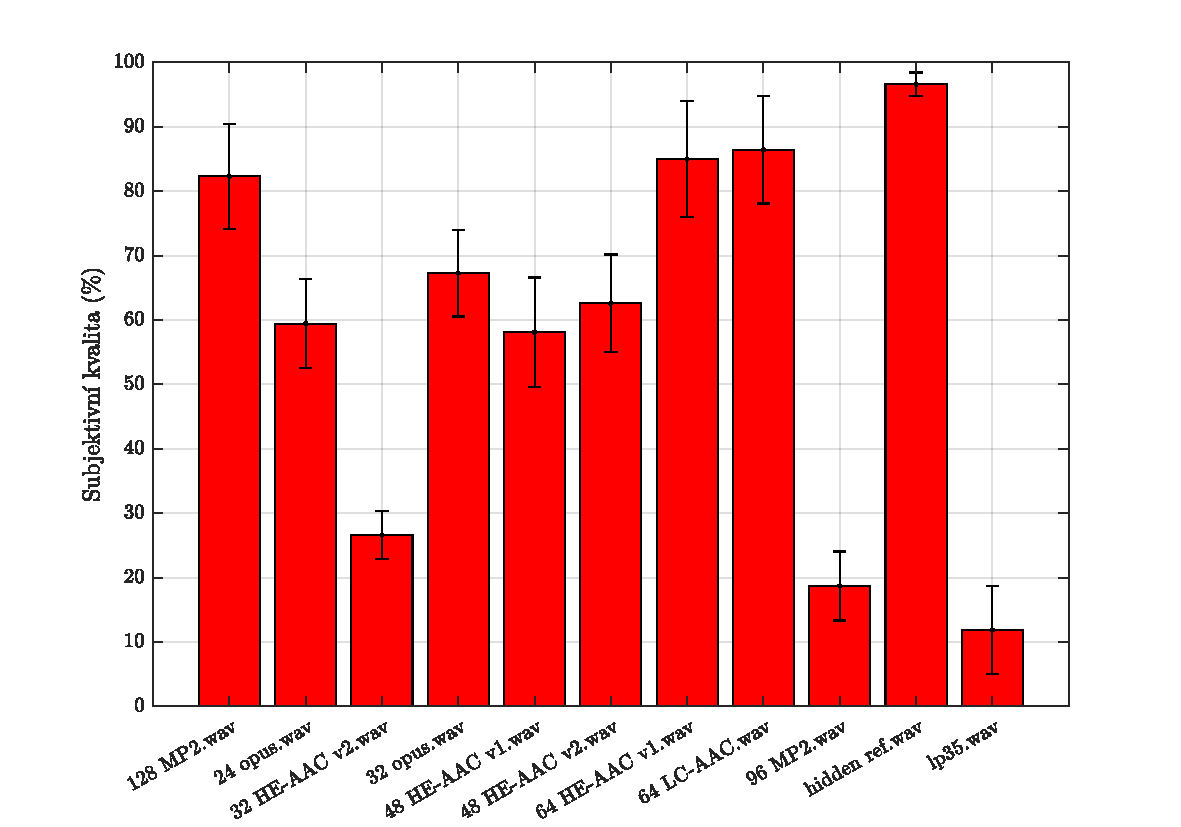
\includegraphics[width = 1\textwidth]{pic/mushra1Mean.pdf}
    \caption{Grafické zobrazení výsledků prvního testu}
    \label{pic:mushra1}
\end{figure}

\begin{figure}[h!]
    \centering
    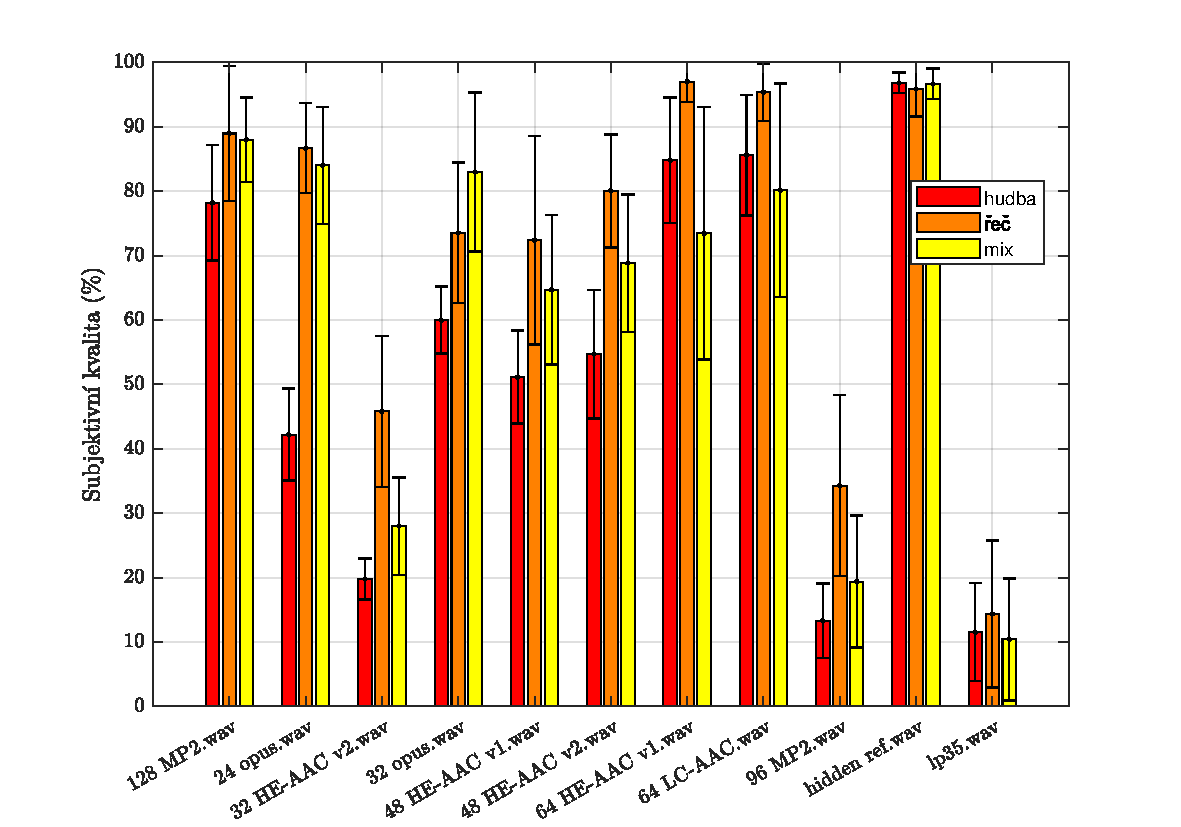
\includegraphics[width = 1\textwidth]{pic/mushra1.pdf}
    \caption{Grafické zobrazení výsledků prvního testu rozdělené do kategorií}
    \label{pic:mushra1:kat}
\end{figure}


\begin{table}[h]
\centering
\begin{tabular}{|c|c|c|c|c|c|c|c|c|c|}
\hline
 & \rot{12 Opus} & \rot{12 xHE-AAC} & \rot{24 HE-AAC v2} & \rot{24 Opus} & \rot{48 HE-AAC v2} & \rot{64 HE-AAC v2 } & \rot{8 xHE-AAC} & \rot{hidden} & \rot{lp35} \\ \hline
$\overline{u}_{k}$ & 24,7 & 48,2 & 27,8 & 68,6 & 61,0 & 65,5 & 28,5 & 97,1 & 16,0 \\ \hline
$\delta_{k}$ & 8,0 & 11,1 & 10,3 & 6,1 & 15,0 & 6,7 & 11,9 & 2,5 & 8,9 \\ \hline
$\overline{u}_{jk(music)}$ & 14,3 & 57,0 & 31,3 & 53,6 & 58,6 & 59,5 & 43,3 & 95,1 & 13,6 \\ \hline
$\delta_{jk(music)}$ & 11,1 & 25,6 & 12,6 & 17,0 & 23,3 & 18,3 & 20,5 & 6,2 & 7,7 \\ \hline
$\overline{u}_{k(speech)}$ & 40,9 & 68,2 & 25,1 & 82,0 & 68,3 & 68,3 & 29,5 & 97,8 & 24,3 \\ \hline
$\delta_{k(speech)}$ & 12,5 & 18,1 & 11,9 & 7,0 & 14,1 & 15,3 & 13,3 & 2,1 & 13,8 \\ \hline
$\overline{u}_{k(mixed)}$ & 18,9 & 19,4 & 26,8 & 70,3 & 56,0 & 68,7 & 12,8 & 98,4 & 10,2 \\ \hline
$\delta_{k(mixed)}$ & 9,9 & 7,5 & 11,0 & 14,1 & 12,1 & 9,2 & 9,1 & 2,2 & 8,3 \\ \hline
\end{tabular}
\caption{Výsledky druhého testu}
\label{table:mos:test2}
\end{table}

\begin{figure}[h!]
    \centering
    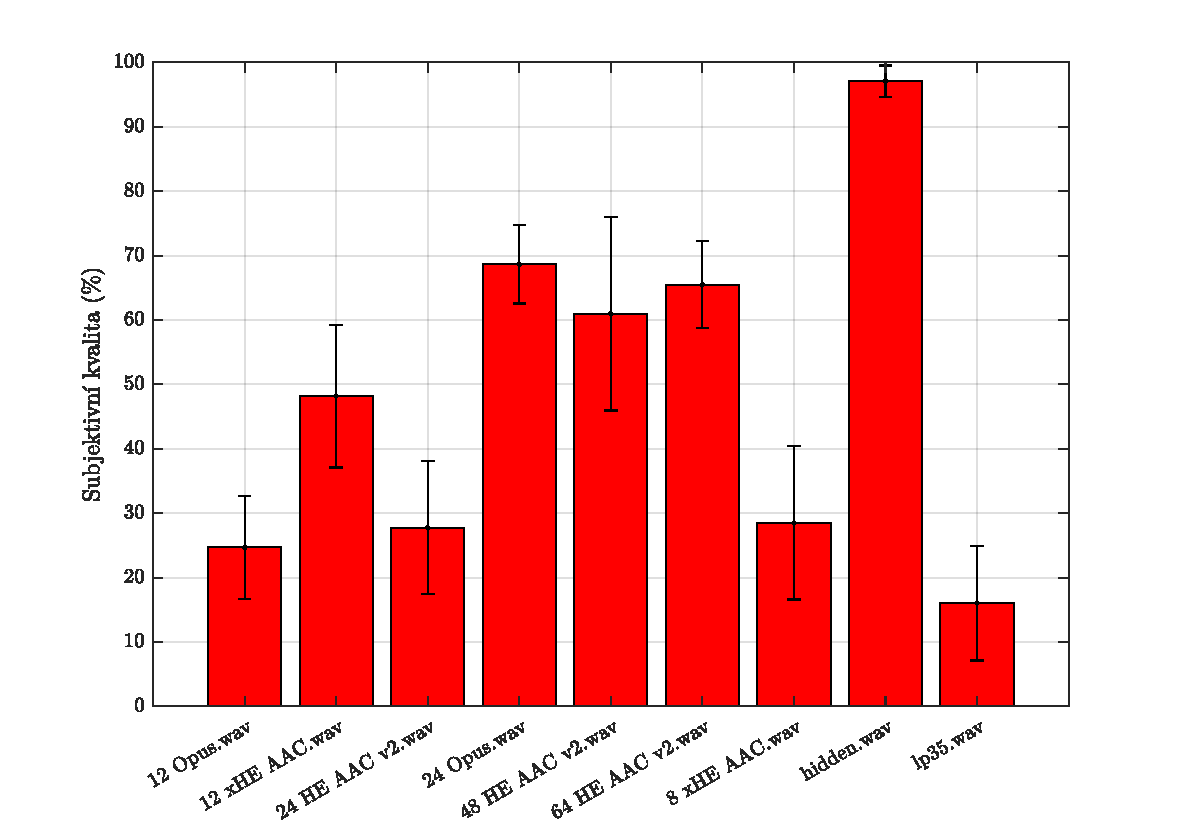
\includegraphics[width = 1\textwidth]{pic/mushra2Mean.pdf}
    \caption{Výsledky testu MUSHRA pro nižší bitové rychlosti}
    \label{pic:mushra2}
\end{figure}

\begin{figure}[h!]
    \centering
    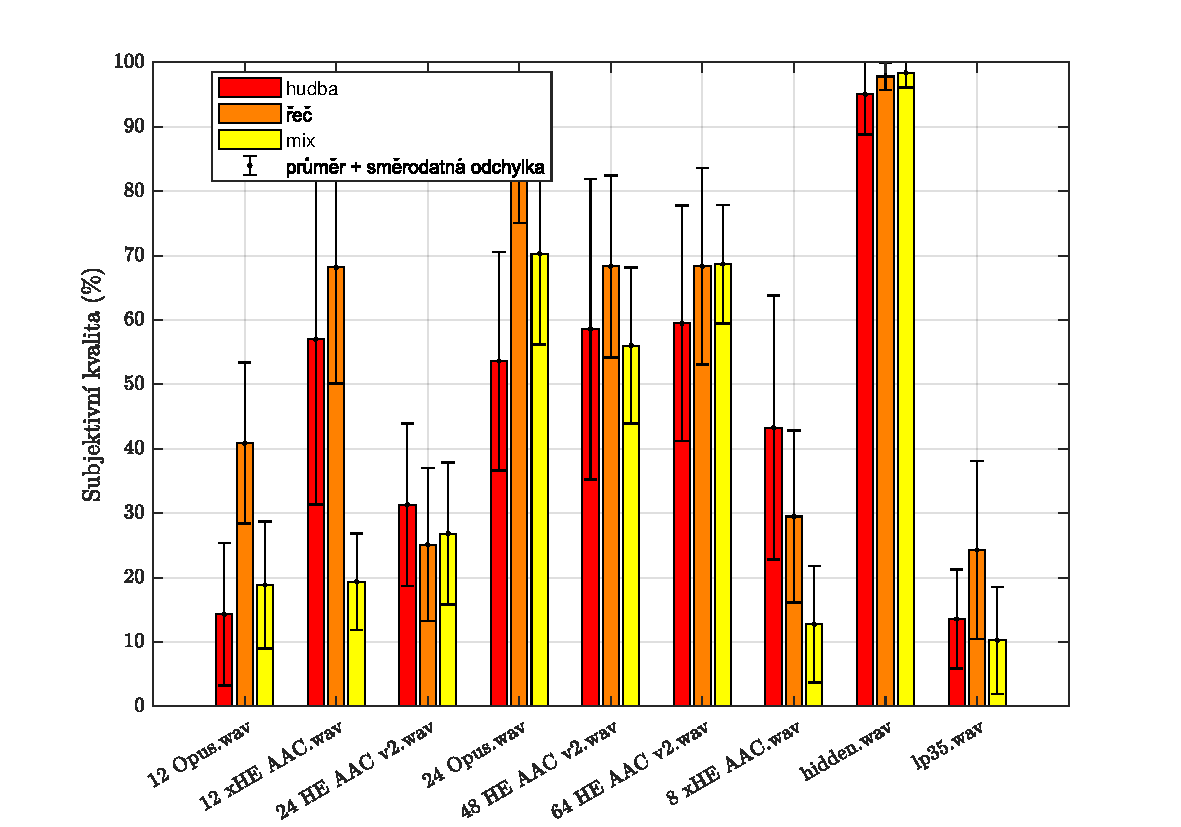
\includegraphics[width = 1\textwidth]{pic/mushra2.pdf}
    \caption{Výsledky testu MUSHRA pro nižší bitové rychlosti včetně kategorií}
    \label{pic:mushra2:kat}
\end{figure}

Jako ukazatel výpovědní hodnoty dosažených výsledků lze brát shodu v hodnocení vzorků konzistentních pro oba testy (zeleně vyznačených v tabulkách \ref{table:test1} a \ref{table:test2}). Průměrné hodnocení stimulů zakódovaných kodekem HE-AAC v2 o bitové rychlosti 48 kb/s dosáhlo hodnot $\overline{u} = 62,6 \%$ s velikostí intervalu spolehlivosti $2\delta = 15 \%$ pro první test a $\overline{u} = 61 \%$ v intervalu s velikostí $2\delta = 30 \%$ pro test druhý. Druhý set vzorků určených pro kontrolu hodnocení mezi dvěma testy byl zkomprimován kodekem Opus s bitovou rychlostí 24 kb/s. Průměrné hodnocení posluchačů v prvním testu $\overline{u} = 59,4 \%$ na intervalu $2\delta = 13,8 \%$ se s průměrnou hodnotou získanou druhým testem $\overline{u} = 68,4 \%$ na intervalu $2\delta = 12,2 \%$ shoduje o něco méně než v prvním případě, se stále však jedná o srovnatelné hodnoty.

Nejlepší hodnocení získala v obou testech skrytá reference a nejhorší skrytá kotva. MPEG Layer II na 96 kb/s dopadl jen o málo lépe než signál omezený dolní propustí o nominálním kmitočtu 3,5 kHz, jelikož při nedostatečné bitové rychlosti jeho psychoakustický model poměrně agresivně kvantizuje vyšší kmitočty a chová se tak jako dolní propust.

Mezigenerační souboje členů rodiny AAC naznačují, že použití metody \textit{Spectral Band Replication} na rychlosti 64 kb/s nepřináší významné vylepšení subjektivně vnímané kvality. Její růst o pár procentních bodů na hodnotící škále lze ovšem sledovat na rychlosti 48 kb/s při použití parametrického sterea. Při poklesu bitové rychlosti na 32/kb už ovšem kvalita padá do oblasti označené jako \uv{špatná}. Proti tomu kodek Opus na stejných rychlostech dosahuje výsledků o zhruba jednu až dvě kvalitativní úrovně výše.

S výjimkou kodeku Opus, u kterého na vyšších rychlostech dopadají nejlépe smíšené vzorky, hodnotí posluchači hudební vzorky hůře než nahrávky z kategorií mluvené slovo a smíšené vzorky. Řeč je ovšem z frekvenčního hlediska méně komplexní než hudba a tak se u ní projevují kompresní artefakty ve srovnání se zakódovanou hudbou méně, i při použití kodeků které nejsou přímo určené ke kompresi mluveného slova. Při započítání překryvů intervalů spolehlivosti dosahují rozdíly v hodnocení jednotlivých kategorií maximálně deseti procent. Celkově se dá pozorovat, že s klesající bitovou rychlostí roste rozptyl získaných hodnot. V testu na nižších bitových rychlostech dosahuje velikost intervalu spolehlivosti hodnoty až $ 2\delta = 30 \%$.

Co druhý test nepotvrdil je výhoda sjednoceného kódování řeči a hudby profilem xHE-AAC. U obou testovaných bitových rychlostí dopadl smíšený vzorek nejhůře ze všech třech kategorií a to s více než desetiprocentní ztrátou oproti průměrné hodnotě. U kodeku Opus dopadají nejlépe téměř výhradně vzorky řečové. Celkově ale xHE-AAC dosahuje vyšší kvality při nízkých rychlostech ve srovnání s ostatními použitými kodeky.

Pokud by tento test měl sloužit jako výběr ideálního kandidáta pro přenos signálu digitálním rádiem, nebyl by zřejmě příliš úspěšný, neboť jen minimum vzorků dosahuje úrovně \uv{Vynikající} či \uv{Dobrá}. Spíše se výsledky pohybují od hladiny 80 \% níže, až po úroveň označovanou jako nedostatečná. Toto \uv{rozprostření} výsledků přes všechny možné úrovně se však hodí pro porovnávání výsledků získaných objektivními algoritmy. Zvýší se tím výpovědní hodnota grafů v následující podkapitole.


\section{Porovnání objektivních a subjektivních výsledků}

Při určování věrohodnosti objektivních metod jsou brány výsledky subjektivních testů jako referenční ukazatel kvality. Při výpočtech a zobrazení je počítáno s aritmetickým průměrem hodnot subjektivně vnímané kvality přes množinu všech subjektů. Všemi předem zmíněnými algoritmy byl za pomocí skriptů popsaných v kapitole \ref{chap:realization} ohodnocen stejný set vzorků jako při poslechových testech. Grafy na obrázku \ref{fig:compare} zobrazují závislost hodnocení kvality objektivními algoritmy na subjektivně vnímané kvalitě pro jednotlivé hodnotící metody. Po vzoru článku \textit{Objective Assessment of Perceptual Audio Quality Using ViSQOLAudio} \cite{article:assessment} byly výsledky všech testů přepočítány na stejnou míru, respektive zobrazeny na stejné škále, aby bylo porovnání přehledné a objektivní. U subjektivních testů byla lineární sto-dílková škála $CQS$ jednoduchým vydělením přepočtena na $SDG$. PEAQ a PEMO-Q poskytují výsledky ve formě $ODG$ a na tu byly přepočítány i výsledky algoritmu ViSQOL, přepočtem z jeho standardního výstupu $MOS\text{-}LQO$. Barevně a za pomocí znaků jsou v nich odlišené metody komprese. Těm je rovněž přidělená eliptická oblast, kde poloosa ve vodorovném směru odpovídá směrodatné odchylce výsledků subjektivních testů a svislá poloosa odpovídá směrodatné odchylce objektivních hodnocení zároveň uvedených v tabulce \ref{table:sigma}. 

Jelikož ideální případ závislosti $ODG$ na $SDG$ je jejich rovnost (čerchovaná modrá přímka) lze velikost chyby spočítat jejich rozdílem. Z těchto rozdílů lze vypočítat střední kvadratickou chybu $\varepsilon$ (\textit{Root Mean Squared Error}) podle:

\begin{equation}
    {\varepsilon} = \sqrt{\sum_{j=1}^{J}\frac{({ODG_j}-{SDG_j})^2}{J}}
\end{equation}

V tabulce \ref{table:epsilon} je vypočítané $\varepsilon$ pro všechny testované metody komprese pomocí všech objektivních metod a v tabulce \ref{table:epsilon:avg} jsou průměrné hodnoty $\overline{\varepsilon}$ a průměru kodeků používaných v digitálním rádiu $\overline{\varepsilon}_{radio}$.

\tabulinesep=1.3mm
\begin{table}[h]
\centering
\small
\begin{tabu}{|c|c|c|c|c|c|c|c|c|c|c|c|c|c|}
\hline
 & \rot{128 MP2} & \rot{24 opus} & \rot{32 HE-AAC v2} & \rot{32 opus} & \rot{48 HE-AAC v1} & \rot{48 HE-AAC v2 } & \rot{64 HE-AAC v1} & \rot{64 LC-AAC} & \rot{96 MP2} & \rot{8 xHE AAC} & \rot{12 xHE AAC} & \rot{lp35} & \rot{uncompressed} \\ \hline
$\varepsilon_{\text{peaq-a.}}$ & 1,70 & 0,70 & 0,46 & 1,34 & 1,16 & 1,27 & 1,49 & 1,79 & 0,40 & 1,62 & 0,75 & 0,21 & 0,15 \\ \hline
$\varepsilon_{\text{peaq-b.}}$ & 1,19 & 0,99 & 0,45 & 1,23 & 0,96 & 0,35 & 1,31 & 1,77 & 0,42 & 1,61 & 0,63 & 0,57 & 0,15 \\ \hline
$\varepsilon_{\text{pemoq}}$ & 0,46 & 0,48 & 0,45 & 1,67 & 1,04 & 0,99 & 0,97 & 1,30 & 1,02 & 1,68 & 0,73 & 1,19 & 0,15 \\ \hline
$\varepsilon_{\text{visqol}}$ & 0,66 & 1,30 & 1,03 & 0,58 & 0,48 & 0,35 & 0,92 & 1,02 & 1,64 & 1,21 & 0,98 & 0,99 & 0,15 \\ \hline
\end{tabu}
\caption{Kvadratické střední chyby $\varepsilon$ pro jednotlivé kompresní metody}
\label{table:epsilon}
\end{table}

\begin{table}[h]
\centering
\begin{tabu}{|c|c|c|}
\hline
 & $\overline{\varepsilon}$ & $\overline{\varepsilon}_{radio}$ \\ \hline
PEAQ A. & 1,01 & 1,27 \\ \hline
PEAQ B. & 0,89 & 1,04 \\ \hline
PEMO-Q & 0,87 & 1,01 \\ \hline
ViSQOL & 0,87 & 0,90 \\ \hline
\end{tabu}
\caption{Průměrná hodnota $\varepsilon$ a $\varepsilon_{radio}$}
\label{table:epsilon:avg}
\end{table}

\begin{table}[h]
\centering
\small
\begin{tabu}{|c|c|c|c|c|c|c|c|c|c|c|c|c|c|}
\hline
 & \rot{128 MP2} & \rot{24 opus} & \rot{32 HE-AAC v2} & \rot{32 opus} & \rot{48 HE-AAC v1} & \rot{48 HE-AAC v2 } & \rot{64 HE-AAC v1} & \rot{64 LC-AAC} & \rot{96 MP2} & \rot{8 xHE AAC} & \rot{12 xHE AAC} & \rot{lp35} & \rot{uncompressed} \\ \hline
 $\sigma_{\text{peaq-a.}}$ & 0,51 & 0,43 & 0,41 & 0,43 & 0,56 & 0,88 & 0,66 & 0,33 & 0,04 & 0,05 & 0,06 & 0,05 & 0,00 \\ \hline
$\sigma_{\text{peaq-b.}}$ & 0,36 & 0,61 & 0,52 & 0,61 & 0,74 & 0,80 & 0,69 & 0,74 & 0,23 & 0,27 & 0,42 & 0,33 & 0,00 \\ \hline
$\sigma_{\text{pemoq}}$ & 0,18 & 0,31 & 0,52 & 0,31 & 0,54 & 1,18 & 0,44 & 0,29 & 0,18 & 0,04 & 0,04 & 0,46 & 0,00 \\ \hline
$\sigma_{\text{visqol}}$ & 0,11 & 0,28 & 0,63 & 0,28 & 0,15 & 0,72 & 0,28 & 0,19 & 0,07 & 0,46 & 0,41 & 0,51 & 0,00 \\ \hline
\end{tabu}
\caption{Směrodatné odchylky objektivního hodnocení}
\label{table:sigma}
\end{table}


\begin{figure}[h!]
    \centering
    \begin{subfigure}{.5\textwidth}
        \centering
        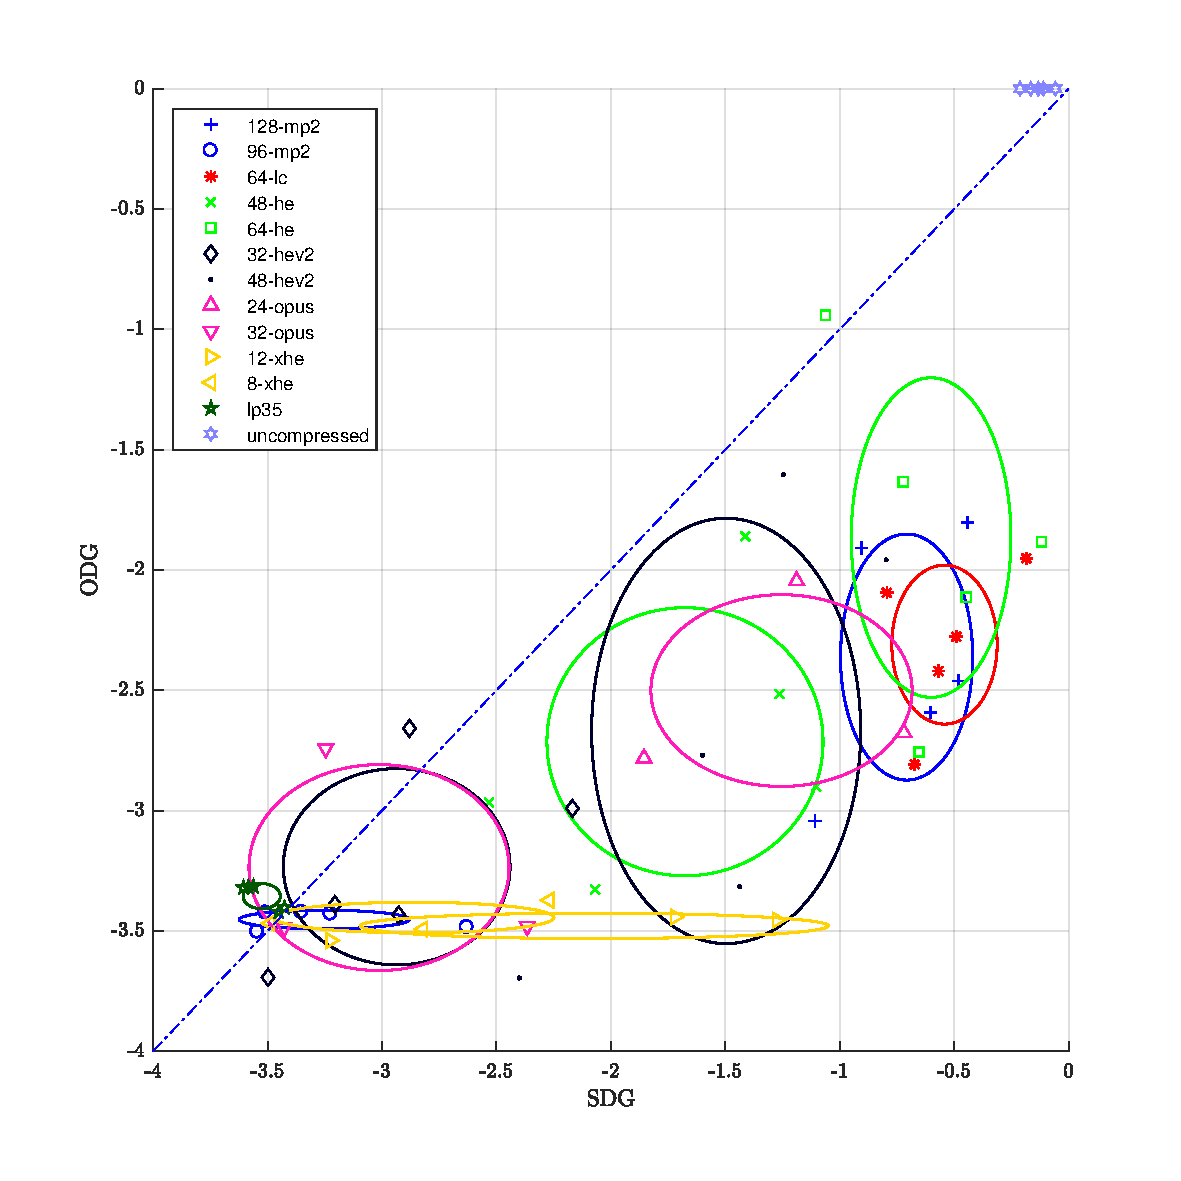
\includegraphics[width=1\linewidth]{pic/compareAdvanced.pdf}
        \caption{PEAQ Advanced}
        \label{fig:compare:advanced}
    \end{subfigure}%
    \begin{subfigure}{.5\textwidth}
        \centering
        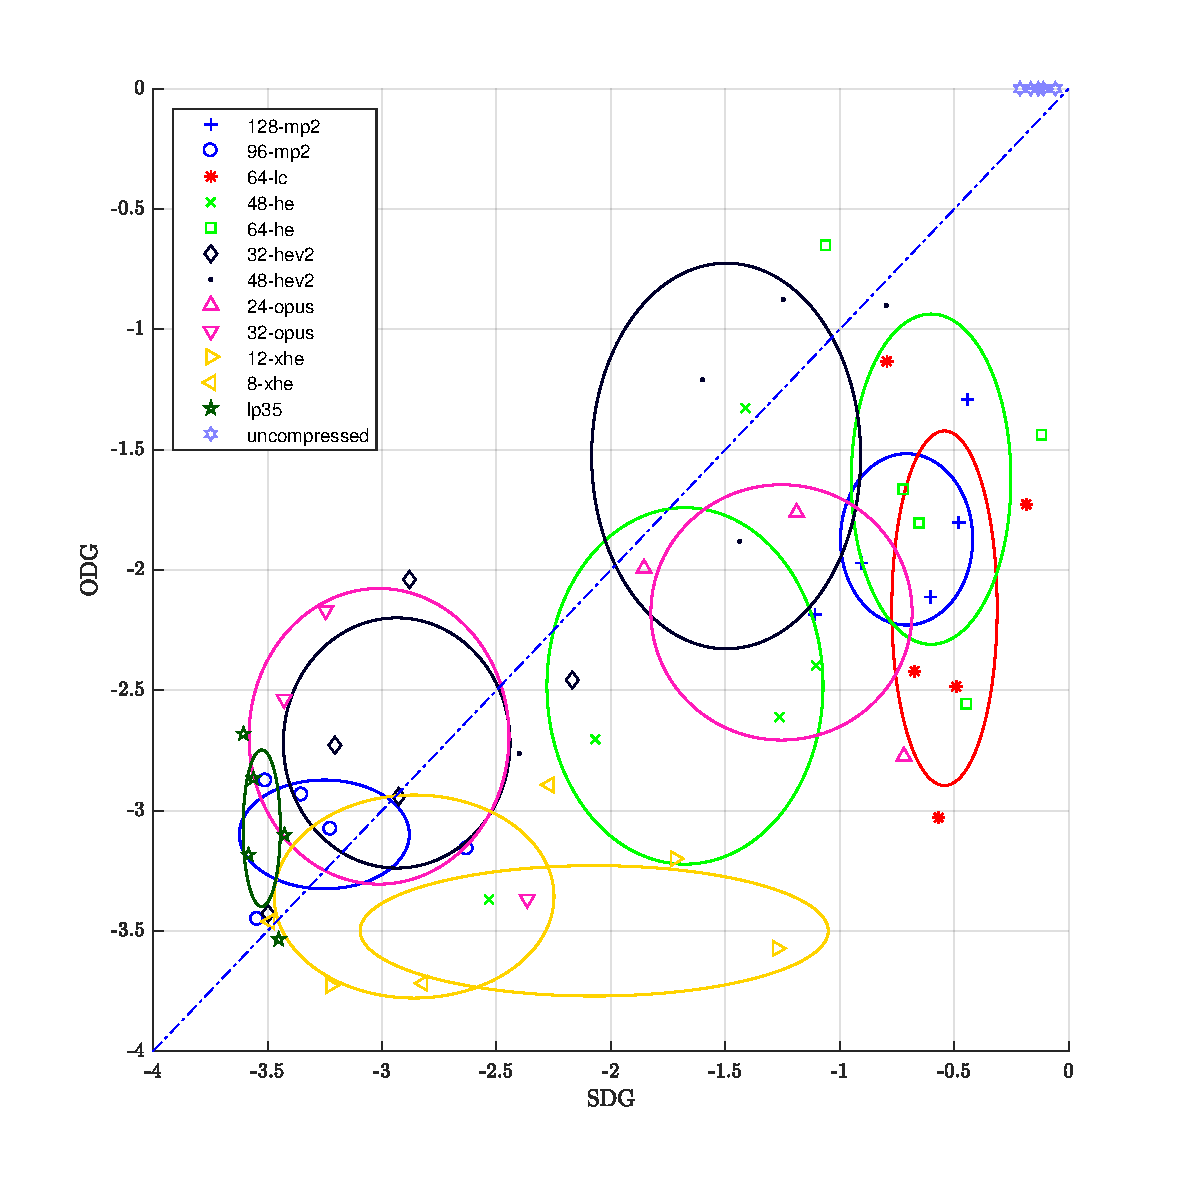
\includegraphics[width=1\linewidth]{pic/compareBasic.pdf}
        \caption{PEAQ Basic}
        \label{fig:compare:basic}
    \end{subfigure}
    \\
        \begin{subfigure}{.5\textwidth}
        \centering
        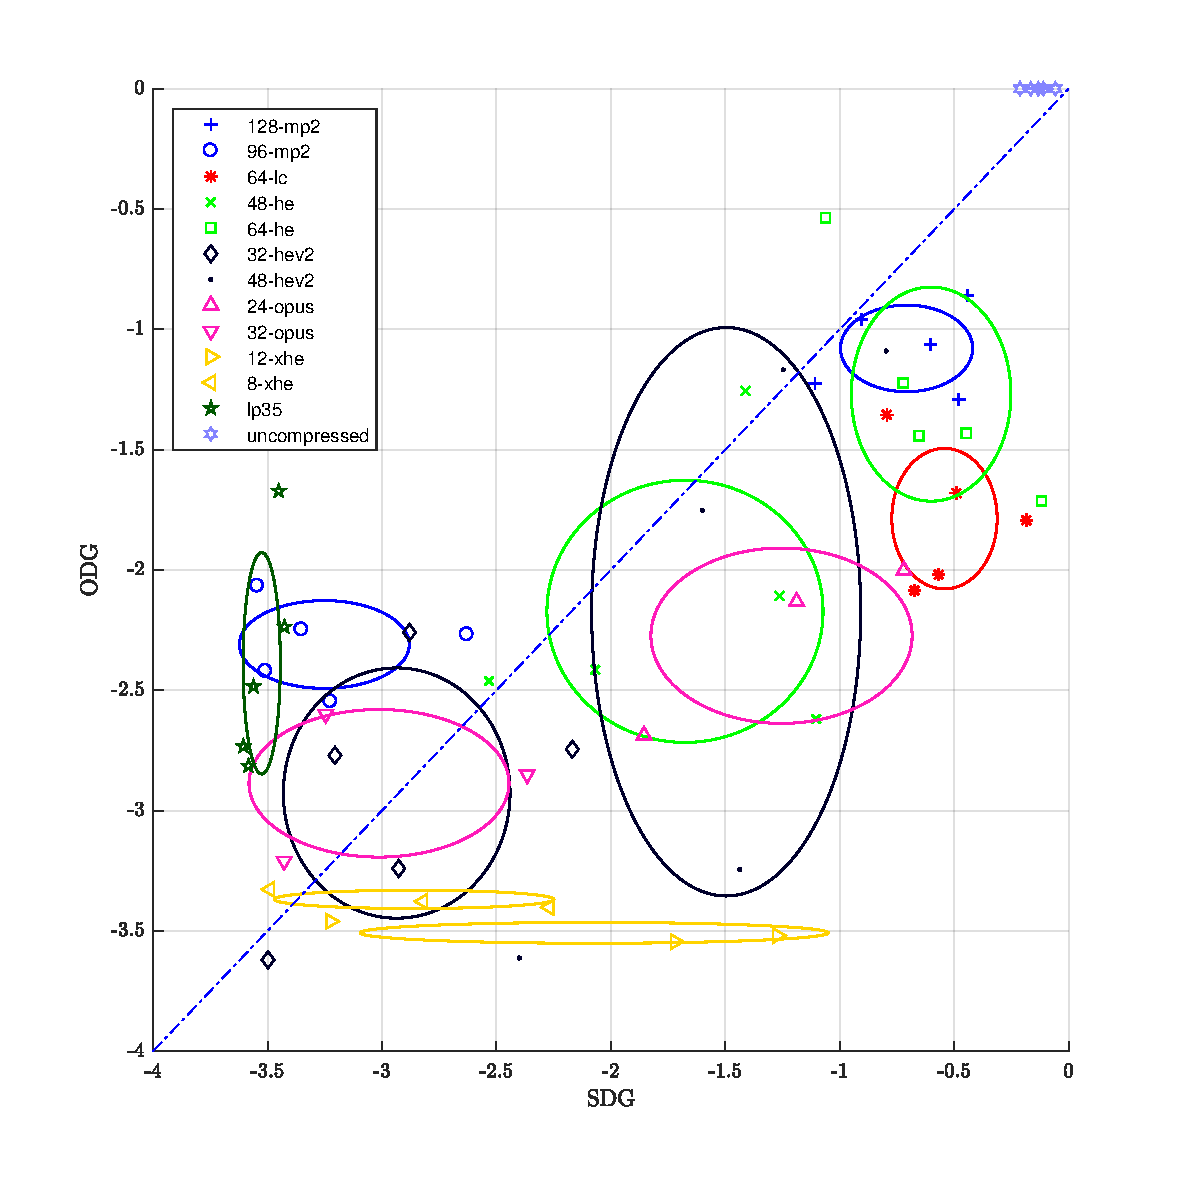
\includegraphics[width=1\linewidth]{pic/comparePemoq.pdf}
        \caption{PEMO-Q}
        \label{fig:compare:pemoq}
    \end{subfigure}%
        \begin{subfigure}{.5\textwidth}
        \centering
        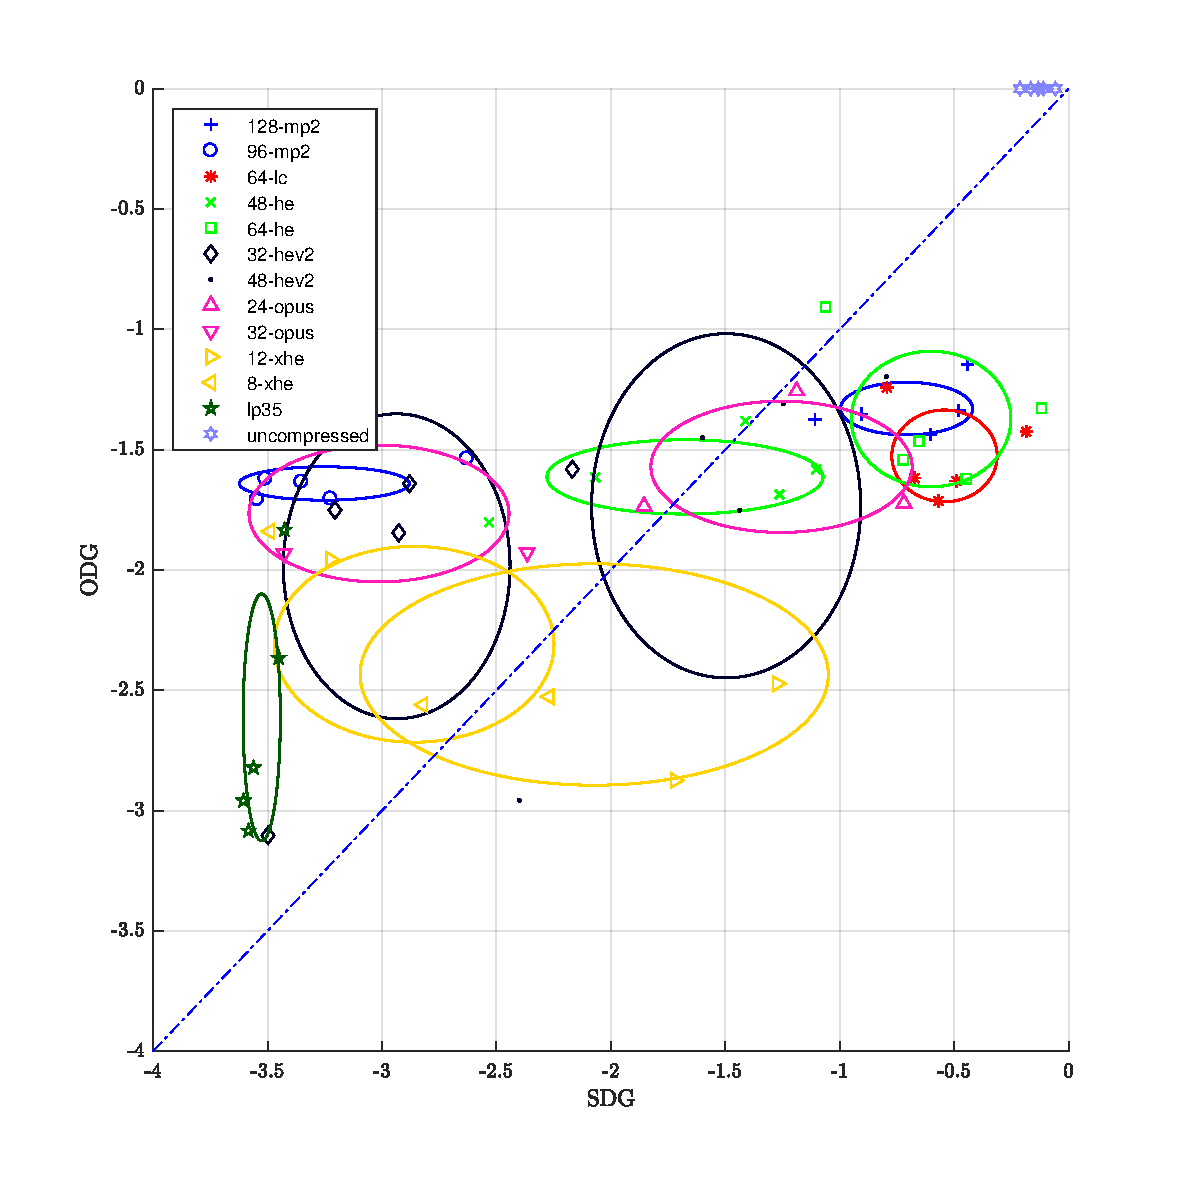
\includegraphics[width=1\linewidth]{pic/compareVisqol.pdf}
        \caption{ViSQOL}
        \label{fig:comapre:visqol}
    \end{subfigure}%
    \caption{Závislost ODG na SDG včetně oblastí vytyčených směrodatnými odchylkami objektivních a subjektivních testů}
    \label{fig:compare}
\end{figure}

Zjednodušeně řečeno, tabulka \ref{table:epsilon} říká, jak moc se jednotlivé algoritmy \uv{mýlí} a tabulka \ref{table:sigma} ukazuje, jak moc náhodné výsledky poskytují.

Bráno podle stáří, hodnocení vzorků zkomprimovaných kodekem MPEG Layer II dosahuje nízkých hodnot rozptylu přes různé druhy nahrávek. Na nižší použité rychlosti 96 kb/s hodnotí s nejmenší chybou oba zástupci algoritmu PEAQ. U PEMO-Q došlo k nadhodnocení o jeden stupeň $ODG$ a u algoritmu ViSQOL je tato hodnota ještě vyšší. Jak už bylo řečeno, MPEG Layer II se při nízkých rychlostech chová jako dolní propust, která mění spektrogram (současně tedy i neurogram) jen nepatrně, díky čemuž je \uv{políčková podobnost} vyšší než u modernějších kompresních metod. PEAQ a na něm založené PEMO-Q zřejmě přikládá vetší váhu gammatónovým filtrům modelu ucha na vysokých kmitočtech, a tak hodnotí \textit{mp2} věrněji. Na druhou stranu při vyšší bitové rychlosti je kvalita MPEG Layer II podhodnocena právě algoritmem PEAQ. Nejmenší chybu poskytl PEMO-Q a druhou nejmenší ViSQOL.

Základní profil AAC LC tvoří v grafech \ref{pic:res:Visqol} zastoupen jen jednou oblastí o bitové rychlosti 64 kb/s, kterou obě verze algoritmu PEAQ podhodnotili o více než jeden stupeň na ODG škále. Základní verze má navíc ze všech algoritmů jednoznačně nejvyšší rozptyl. Nejkonzistentnější výsledek a zároveň nejmenší chybu poskytl ViSQOL. 

Pokud se k základnímu profilu AAC přidá rozšíření SBR, projevuje se to poklesem kvadratické chyby a současným vzrůstem směrodatné odchylky u všech metod. Tento trend dál pokračuje i s poklesem rychlosti HE-AAC v1 na 48 kb/s, kromě hodnocení algoritmu ViSQOL u kterého rozptyl naopak klesá. Také chybu udává nejmenší a to $\varepsilon = 0,48$.

Dalším generačním krokem k HE-AAC v2 kvadratická chyba roste u algoritmů PEAQ a PEMO-Q, zatímco u hodnocení metodou ViSQOL chyba opět klesá. U tohoto profilu je nejvyšší rozptyl objektivně změřené kvality. Směrodatná odchylka výsledků algoritmu PEAQ dosahuje téměř 1,2 stupně ODG na obě strany od průměru. PEAQ Advanced poskytuje hodnotu $\sigma = 0,88$ a ViSQOL $\sigma = 0,72$. Oblast s nižší rcyhlostí 32 kb/s HE-AAC v2 protíná ideální převodní křivku ve třech případech ze čtyř. Jen hodnocení algoritmem ViSQOL je vyšší než u subjektivních testů a to o jeden stupeň ODG.

Kodek Opus v digitálních rádiích nefiguruje a proto jeho hodnocení nemá vliv na jakýkoliv výsledný verdikt. Na nižší rychlosti 24 kb/s ho s nejmenší chybou hodnotil algoritmus PEMO-Q a při vyšším toku 32 kb/s ViSQOL, který dosáhl taktéž nejmenší směrodatné odchylky u obou rychlostí.

Téměř zázračně nízké hodnoty směrodatné odchylky u kodeku xHE-AAC jsou způsobeny spíše tím, že PEAQ ani PEMO-Q si s jeho hodnocením neví příliš rady a tak všem testovaným vzorkům přiřadili hodnotu $ODG \approx 3,5$. Jediný ViSQOL dosahuje hodnocení, které se přibližuje výsledkům subjektivních testů.

Trochu mimo dosavadní výběr stojí dvě poslední oblasti a to skrytá kotva a skrytá reference. Jsou ovšem součástí výstupu subjektivního testování a není důvod nezařadit je do těchto závislostí po bok kompresních metod. Referenční vzorek všechny algoritmy ohodnotily bez jakékoliv ztráty kvality a tak se eliptická oblast zjednodušila na úsečku v pravém horním rohu grafů \ref{pic:res:Visqol}. Signál s potlačenými kmitočty od 3,5 kHz výše stejně jako posluchači ohodnotily obě verze algoritmu PEAQ. ViSQOL i PEMO-Q skrytou kotvu nadhodnocují zhruba o jeden stupeň ODG.

Ani jedna z metod neposkytuje ideální výsledky. Lze ale vysledovat trend, že algoritmy PEAQ a PEMO-Q poskytují horší výsledky u modernějších kodeků používaných v digitálních rádiích zatímco ViSQOL má problémy spíše s nadhodnocováním vzorků, které postrádají vyšší harmonické. ViSQOL také v průměru hodnotí s nejmenší kvadratickou chybou, což je ještě výraznější u průměrné hodnoty $\varepsilon_{radio}$, ve které jsou zahrnuty kodeky používané v DRM(+) a DAB/DAB+. Na základě těchto poznatků je označen za nejobjektivnější hodnotící metodu ze všech prezentovaných.

\section{Výsledky objektivních testů}

V zadání této práce je mimo jiné zmíněno, že vybraná objektivní metoda by měla být využita pro vyhodnocení kvality zvuku v systémech digitálního rozhlasového vysílání. Z algoritmizačního hlediska bylo jednodušší vyhodnotit kvalitu všemi metodami, pro všechny kodeky a všechny možné bitové rychlosti a naimportovat je pomocí skriptu \code{makeCell} do zobrazovacího nástroje \code{showResults}. Protože v předchozí podkapitole je jako nejvěrohodnější objektivní metoda vybrán ViSQOL, potažmo jeho varianta ViSQOLAudio jsou v tomto textu tedy vybrány pouze závislosti vygenerované algoritmem ViSQOL. 

Výsledky z ostatních algoritmů jsou k nahlédnutí v dodatku \ref{app:3}, či v samotném nástroji \code{showResults}, kde si může uživatel výstup libovolně nakonfigurovat a exportovat do souboru.

Obrázek \ref{pic:res:Visqol} obsahuje šestici grafů zobrazující průměrné $ODG$ a směrodatnou odchylku všech vzorků z tabulky \ref{table:material}. Do nich jsou rovněž vyneseny výsledky poslechových testů pro lepší představu toho jak spolu korespondují. Pro DRM+ a DAB+ jsou klíčové grafy \ref{fig:vis:sub1} a  \ref{fig:vis:sub3} až \ref{fig:vis:sub6}.

Pro hodnocení \textit{MPEG Layer II} není ViSQOL příliš vhodný avšak to je jediný případ, kdy je radno sáhnout po jiné objektivní metodě. Na velmi nízkých bitových rychlostech stále uděluje hodnocení MOS-LQO vyšší než 3, slovně řečeno lepší než přijatelné. Tento kodek je ovšem v současnosti nahrazován pokročilejšími kompresními metodami a tam si ViSQOL vede podstatně lépe.

Podobně jako první subjektivní test ukázal, že mezi generacemi HE-AAC v1 a HE-AAC v2 lidské ucho téměř neslyší rozdíl, hodnotí v průměru ViSQOL tyto dva profily velmi podobně. U HE-AAC v2 nicméně podává výsledky se zhruba o třetinu větším rozptylem. Užití rozšíření PS a SBR má své výhody, ale i rizika. S rostoucím bitovým tokem se kódový zisk nabytý použitím metod založených na psychoakustických poznatcích klesá a v určitém momentu již nastoupí výhody nižšího profilu.

\begin{figure}[H]
    \centering
    \begin{subfigure}{.5\textwidth}
        \centering
        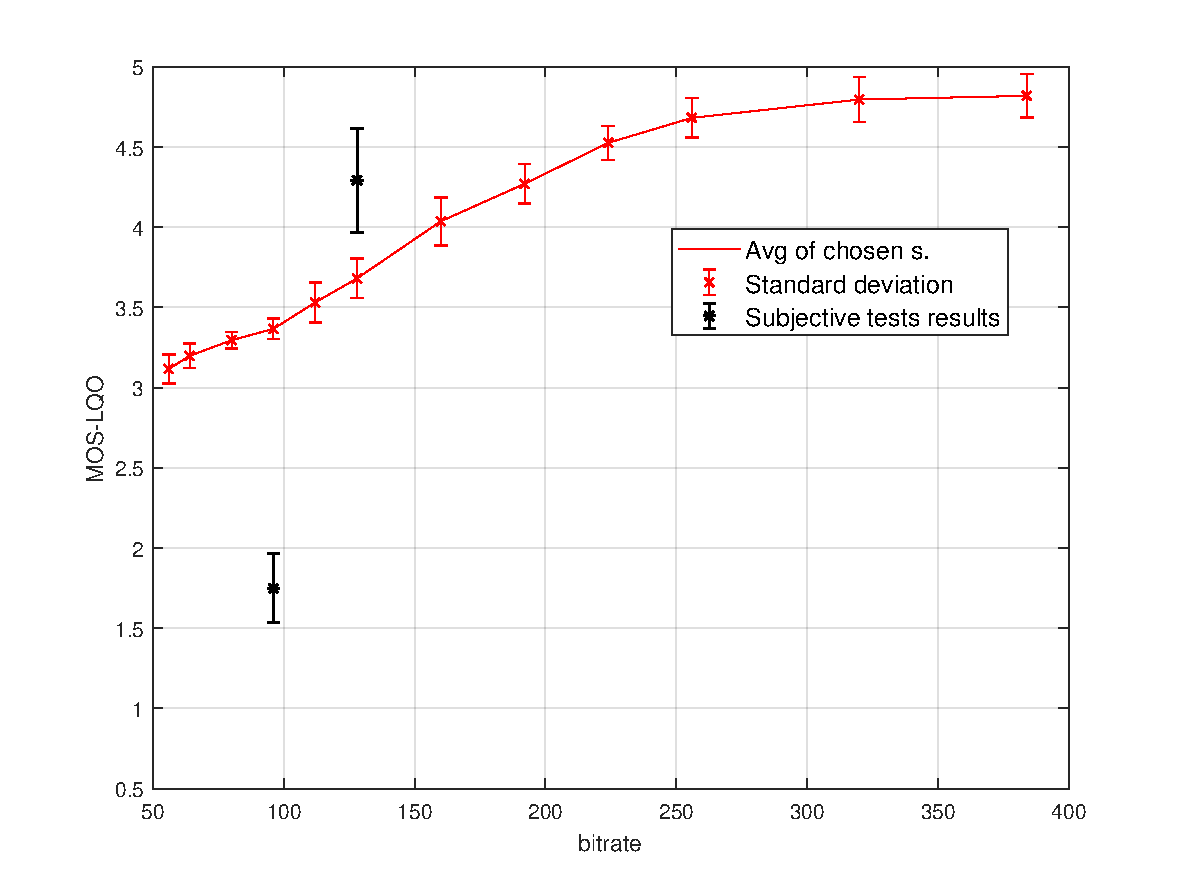
\includegraphics[width=1\linewidth]{pic/objective/mp2Visqol.pdf}
        \caption{MP2}
        \label{fig:vis:sub1}
    \end{subfigure}%
    \begin{subfigure}{.5\textwidth}
        \centering
        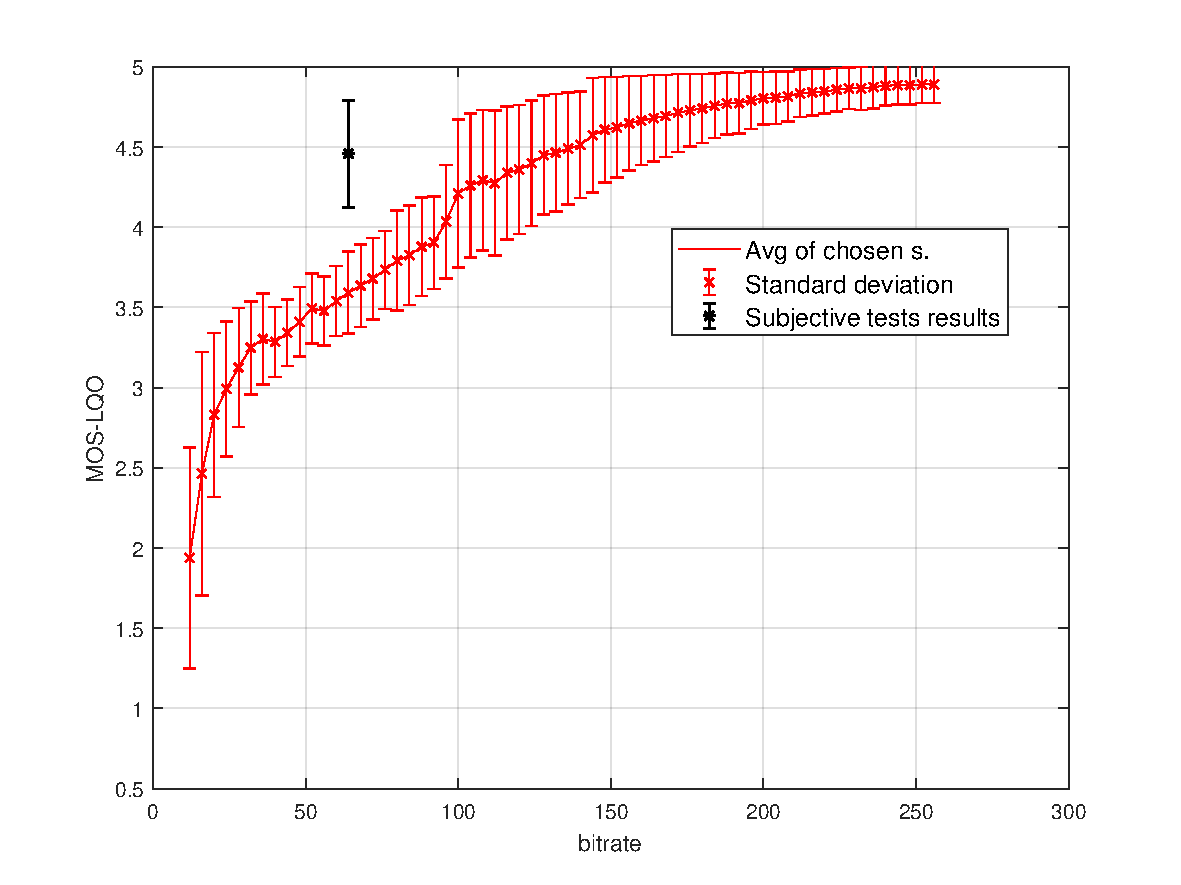
\includegraphics[width=1\linewidth]{pic/objective/lcVisqol.pdf}
        \caption{LC-AAC}
        \label{fig:vis:sub2}
    \end{subfigure}
    \\
%\end{figure}
%\begin{figure}[htb]\ContinuedFloat        
    \begin{subfigure}{.5\textwidth}
        \centering
        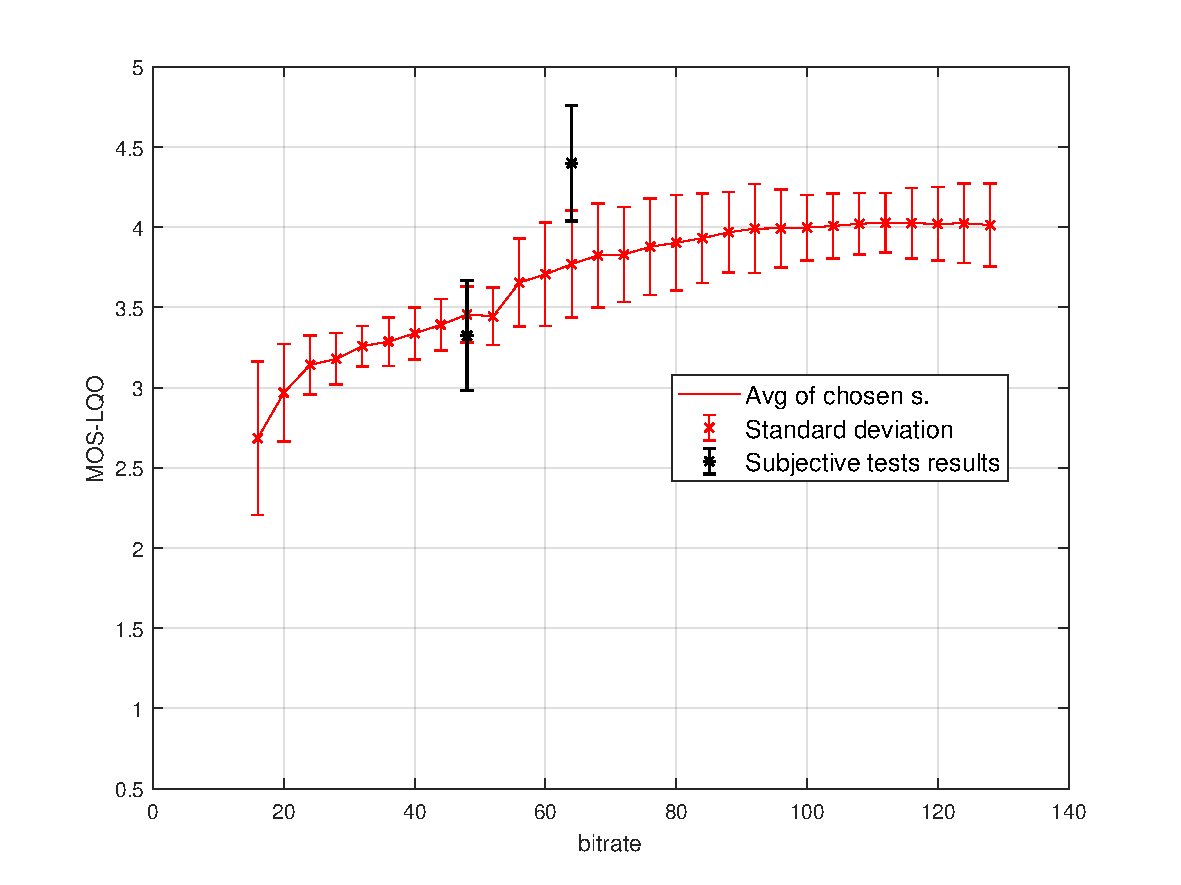
\includegraphics[width=1\linewidth]{pic/objective/heVisqol.pdf}
        \caption{HE-AAC v1}
        \label{fig:vis:sub3}
    \end{subfigure}%
        \begin{subfigure}{.5\textwidth}
        \centering
        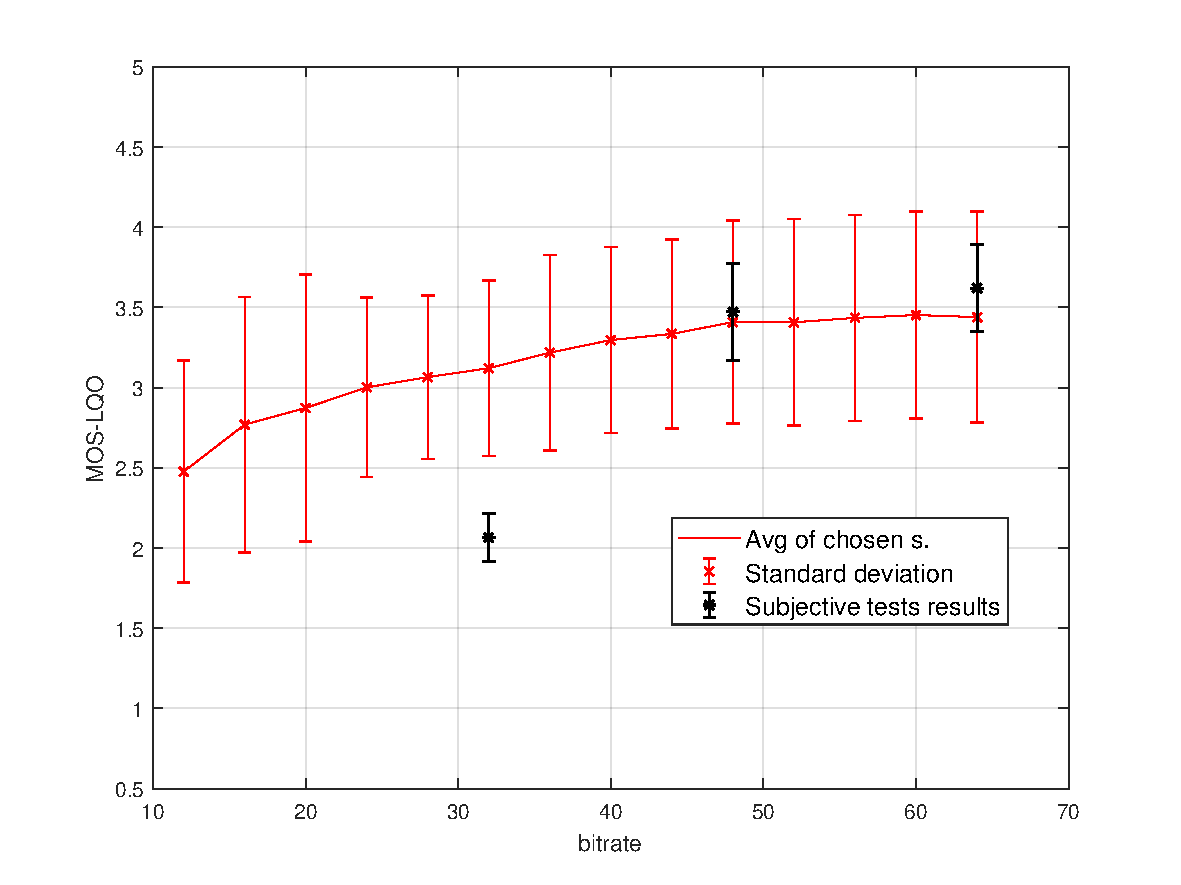
\includegraphics[width=1\linewidth]{pic/objective/hev2Visqol.pdf}
        \caption{HE-AAC v2}
        \label{fig:vis:sub4}
    \end{subfigure}%
    \\
\end{figure}
\begin{figure}[h]\ContinuedFloat
        \begin{subfigure}{.5\textwidth}
        \centering
        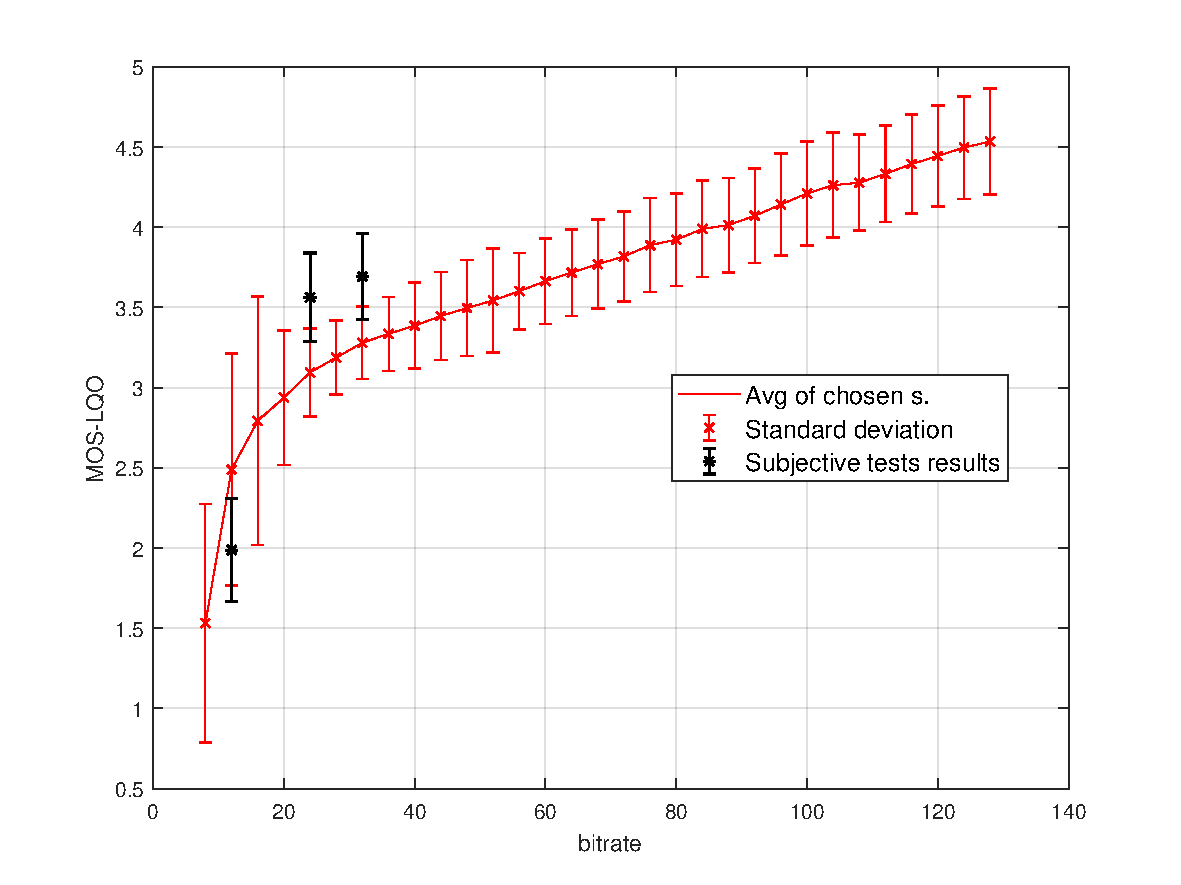
\includegraphics[width=1\linewidth]{pic/objective/opusVisqol.pdf}
        \caption{Opus}
        \label{fig:vis:sub5}
    \end{subfigure}%
        \begin{subfigure}{.5\textwidth}
        \centering
        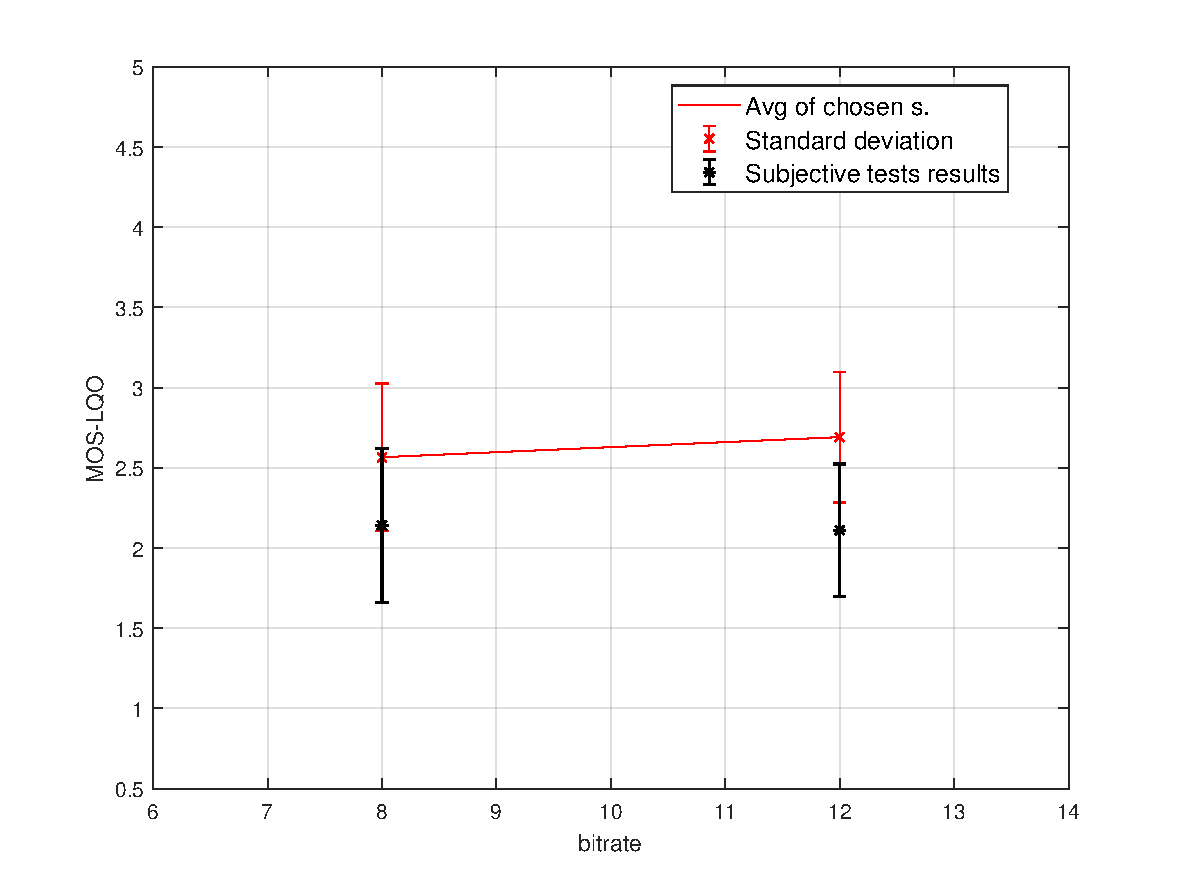
\includegraphics[width=1\linewidth]{pic/objective/xheVisqol.pdf}
        \caption{xHE-AAC}
        \label{fig:vis:sub6}
    \end{subfigure}%
    \caption{Hodnocení algoritmem ViSQOL.} 
\label{pic:res:Visqol}
\end{figure}

\bigskip
\bigskip

I přes to, že k rozhodnutí zvolit právě ViSQOL nevedlo hodnocení vzorků zakódovaných kodekem Opus, je podobnost objektivních a subjektivních výsledků značná.

%Lze očekávat, že v blízké budoucnosti bude svět DRM postupně adaptován na využití kodeku xHE-AAC, který nabízí přijatelnou kvalitu na velmi nízkých rychlostech. Jak si stojí při použití vyšší bitové rychlosti 

Ze závislostí na obrázku \ref{pic:res:Visqol} lze říci, že pokud má být kvalita zvuku přenášeného digitálním rádiem hodnocena posluchači jako vynikající nezbývá než volit z kodeků MPEG Layer II a AAC LC. U prvního ze zmíněných je třeba bitového toku 160 kb/s či více, druhému k překročení spodní hranice vynikající kvality stačí 128 kb/s. Žádná jiná z kompresních metod tohoto kvalitativního prahu nedosahuje. 

Pokud je poskytovatel ochotný slevit ze svých požadavků a vysílat kvalitou označovanou jako dobrá (60 \% - 80 \% na CQS stupnici), dosáhne nejvyšší efektivity volbou profilu HE-AAC v2 na bitové rychlosti 44 kb/s. Kdyby z nějakých důvodů nebylo možné využít rozšíření \textit{Parametric Stereo}, dosáhne stejného výsledku s bitovým tokem 56 kb/s profilů HE-AAC v1 a AAC LC, které na této rychlosti ViSQOL hodnotí stejně. Při použití MPEG Layer II by bylo potřeba dvojnásobného toku 112 kb/s. 

Pokud je prioritou úspora prostředků a padne rozhodnutí vysílat pouze přijatelnou kvalitou, lze dle hodnocení algoritmu ViSQOL využít kompresní metodu xHE-AAC. Pro přenos mluveného slova je dostatečnou bitovou rychlostí 8 kb/s. Při přenosu hudebních záznamů je lepší sáhnout po rychlosti 12 kb/s. Jaké kvality xHE-AAC dosahuje na vyšších tocích bohužel kvůli absenci kodéru nebylo zjištěno. V digitálním rádiu DAB, které xHE-AAC neintegruje lze stejné kvality pro vysílání řeči dosáhnout užitím kodeku HE-AAC v2 s tokem 16 kb/s a pro přenos hudebního obsahu nejméně 20 kb/s.




\widowpenalty=9999
\chapter{Závěr}
\label{chap:conclusion}

\epigraph{\textit{\hfill Nejjednodušší řešení je obvykle to správné.}}{-jedna z interpretací filozofického přístupu známého jako Occamova Břitva}

Tato práce měla několik dílčích cílů. Zpočátku bylo třeba zmapovat metody pro hodnocení zvukového signálu. Dále bylo třeba realizovat a vyhodnotit poslechový test na množině vzorků reprezentující obsah a kompresní metody používané v systémech \textit{Digital Radio Mondiale} a \textit{Digital Audio Broadcasting}. Stejnou množinu vzorků bylo potřeba oznámkovat dostupnými algoritmy pro objektivní hodnocení kvality zvuku a s ohledem na výsledek subjektivních testů vybrat metodu vhodnou pro objektivní hodnocení signálu používaného v digitálních rádiích. Posledním dílčím úkolem bylo za pomoci vybraného hodnotícího postupu posoudit kvalitu zvukových nahrávek v závislosti na bitovém toku a typu použité komprese.

Jelikož digitální rádio je středobodem této práce, jsou mu společně s popisem zdrojového kódování věnovány první dvě kapitoly. Popsány jsou možnosti a principy systémů DAB/DAB+ a DRM(+). Dále je uveden stručný vhled do problematiky kompresních standardů MPEG Layer II, MPEG 4 AAC v profilech AAC LC, HE-AAC v1 a HE-AAC v2, MPEG D xHE-AAC a kodeku Opus, který v systémech digitálního rádia nefiguruje, nicméně sdílí s xHE-AAC sjednocené kódování zvuku a řeči a je tak zajímavým doplňkem.

Konzumentem rozhlasového obsahu byl, je a pravděpodobně vždy bude člověk. Lidský vjem je tak stále nejlepším způsobem jak hodnotit kvalitu zvuku. Proto je určování kvality pomocí poslechu lidskými subjekty věnována celá kapitola. Popsány jsou postupy definované mezinárodní telekomunikační unií od přístupů obecných, přes způsob určování nepatrných zhoršení až po metodu pro střední kvalitu s označením MUSHRA.

Ta je využita při subjektivním testování. Pro určení kvality vzorků, rozdělených do kategorií: hudební, řečové s smíšené, byly navrženy dva mírně se překrývající testy. Jeden sledující kvalitu na vyšších bitových rychlostech starších kodeků, a druhý obsahující materiál zakódovaný moderními kodeky, jenž cílí na velmi nízké bitové toky. Bylo pro ně vyvinuto grafické uživatelské rozhraní v programovacím jazyce \matlab a celkově sedmnáct subjektů absolvovalo oba testy.

Pro generování vzorků, jejich objektivní testování a zobrazování získaných výsledků byla vyvinuta skupina znovupoužitelných skriptů a aplikací, taktéž v prostředí \matlab. Pomocí algoritmů PEAQ Basic, PEAQ Advanced, PEMO-Q a ViSQOL byly ohodnoceny vzorky zakódované všemi již zmíněnými kodeky.

Porovnání subjektivního a objektivního hodnocení odhalilo, že ne vždy lze použít Occamovu břitvu. Žádná z metod totiž není stoprocentně spolehlivá. Nejstarší PEAQ nejlépe hodnotí dnes už historický kodek MPEG Layer II a u novějších kompresních algoritmů klesá věrohodnost jeho hodnocení. PEMO-Q, které algoritmus PEAQ doplňuje o komplexnější model ucha sdílí podobný trend. Nejmodernější ViSQOL, původně vytvořený pro hodnocení řeči v telekomunikacích, si vede lépe u moderních metod komprese. Jako jediný se přibližuje výsledku subjektivního hodnocení vzorků zakódovaných metodou xHE-AAC. Nejstarší MPEG Layer II na nízkém bitovém toku ovšem značně nadhodnocuje. Protože jsou ale starší kodeky vytlačovány novými efektivnějšími kompresními přístupy, jeví se ViSQOL jako nejlepší volba do budoucna.

Zároveň je ale možné, že snížením váhy přikládané výstupům filtrů na vysokých kmitočtech v modelu sluchové cesty u algoritmů PEAQ či PEMO-Q by mohlo vést ke zvýšení věrohodnosti jimi podaných výsledků. Jelikož implementace algoritmů PEAQ Basic, PEMO-Q i ViSQOL byly k dispozici ve formě funkcí pro \matlab, nabízí se do budoucna možnost jejich úprav či propojení, tak aby podávaly věrohodnější hodnocení pro kompletní škálu kompresních metod.

V této práci je za prozatím nejvěrohodnější metodou zvolen ViSQOL. Pomocí něho je ohodnocen kompletní set vzorků, podrobně popsaný v kapitole \ref{chap:realization}. Výsledky jsou s komentářem k dispozici v grafické podobě v poslední kapitole této práce, věnované kvalitě přenosu zvuku v digitálních rádiích. Vynikající poslechové kvality lze při zdrojovém kódování dosáhnout pouze použitím starších kodeků na vyšších bitových rychlostech. Vývoj moderních kodeků se soustřeďuje na zvyšování kódového zisku při zachování dobré, či alespoň přijatelné kvality. Té lze dosáhnout už při datovém toku 8 kb/s pro přenos mluveného slova nebo 12 kb/s pro vysílání hudebních záznamů. Protože jsou vysílací mechanismy digitálního rádia podstatně odolnější vůči analogovému rušení, existuje velmi vysoká pravděpodobnost, že se ke koncovému zákazníkovi dostane zvukový signál ve stejné kvalitě, do jaké byl kompresní metodou zakódován. Ta tak ve výsledku mnohdy předčí kvalitu analogového rádia.
%------------------------------------------------------------------------------------------
% Use bibtex to produce bibliography used in the thesis, except for your own publications
%------------------------------------------------------------------------------------------
\bibliographystyle{iso690}
%\bibliographystyle{abbrv}
% \cleardoublepage\phantomsection\addcontentsline{toc}{chapter}{\protect\numberline{}{Bibliography}}
\bibliography{main}


% list your own books or papers in refereed journals or conference proceedings
% or chapters in scientific monographies that are RELEVANT FOR YOUR THESIS


\appendix

\appendix
\chapter{Digitální přílohy}
\label{app:1}

Na přiloženém CD jsou následující přílohy v digitální podobě:

\begin{itemize}
    \item Skripty pro \matlab:
    \begin{itemize}
        \item \code{main}
        \item \code{makeAac}
        \item \code{makeMp2}
        \item \code{makeOpus}
        \item \code{makeWav}
        \item \code{makeCell}
        \item \code{mushra}
        \item \code{showResults}
    \end{itemize}
    
    \item Vzorky ve zkomprimované a PCM formě
    \item Text práce v PDF
\end{itemize}
\chapter{Přílohy k subjektivnímu testu}
\label{app:2}
\section{Informovaný souhlas}

\begin{figure}[H]
    \centering
    \frame{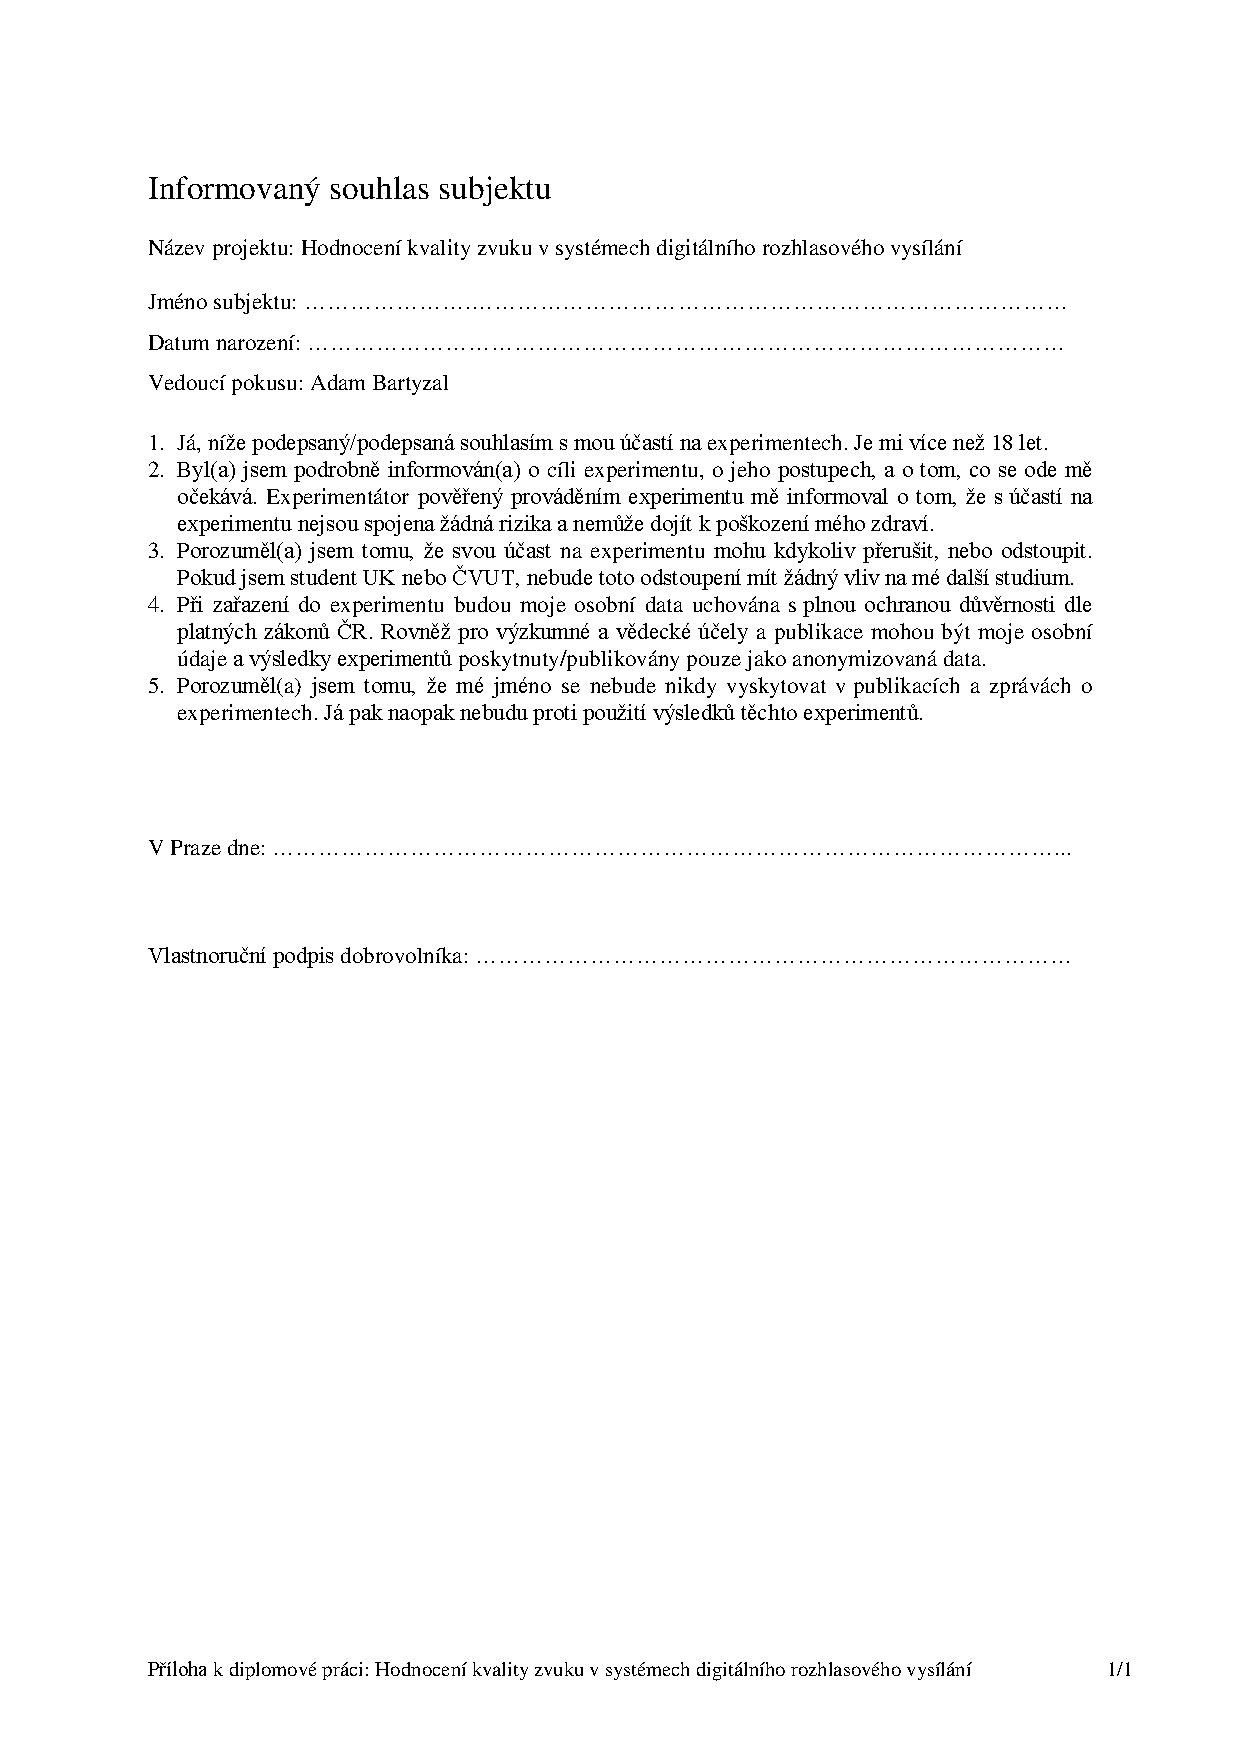
\includegraphics[page=1,width=.55\textwidth]{pdf/agreement.pdf}}
    \label{pdf:agreement}
\end{figure}

\section{Doprovodné informace}

\begin{figure}[H]
    \centering
    \frame{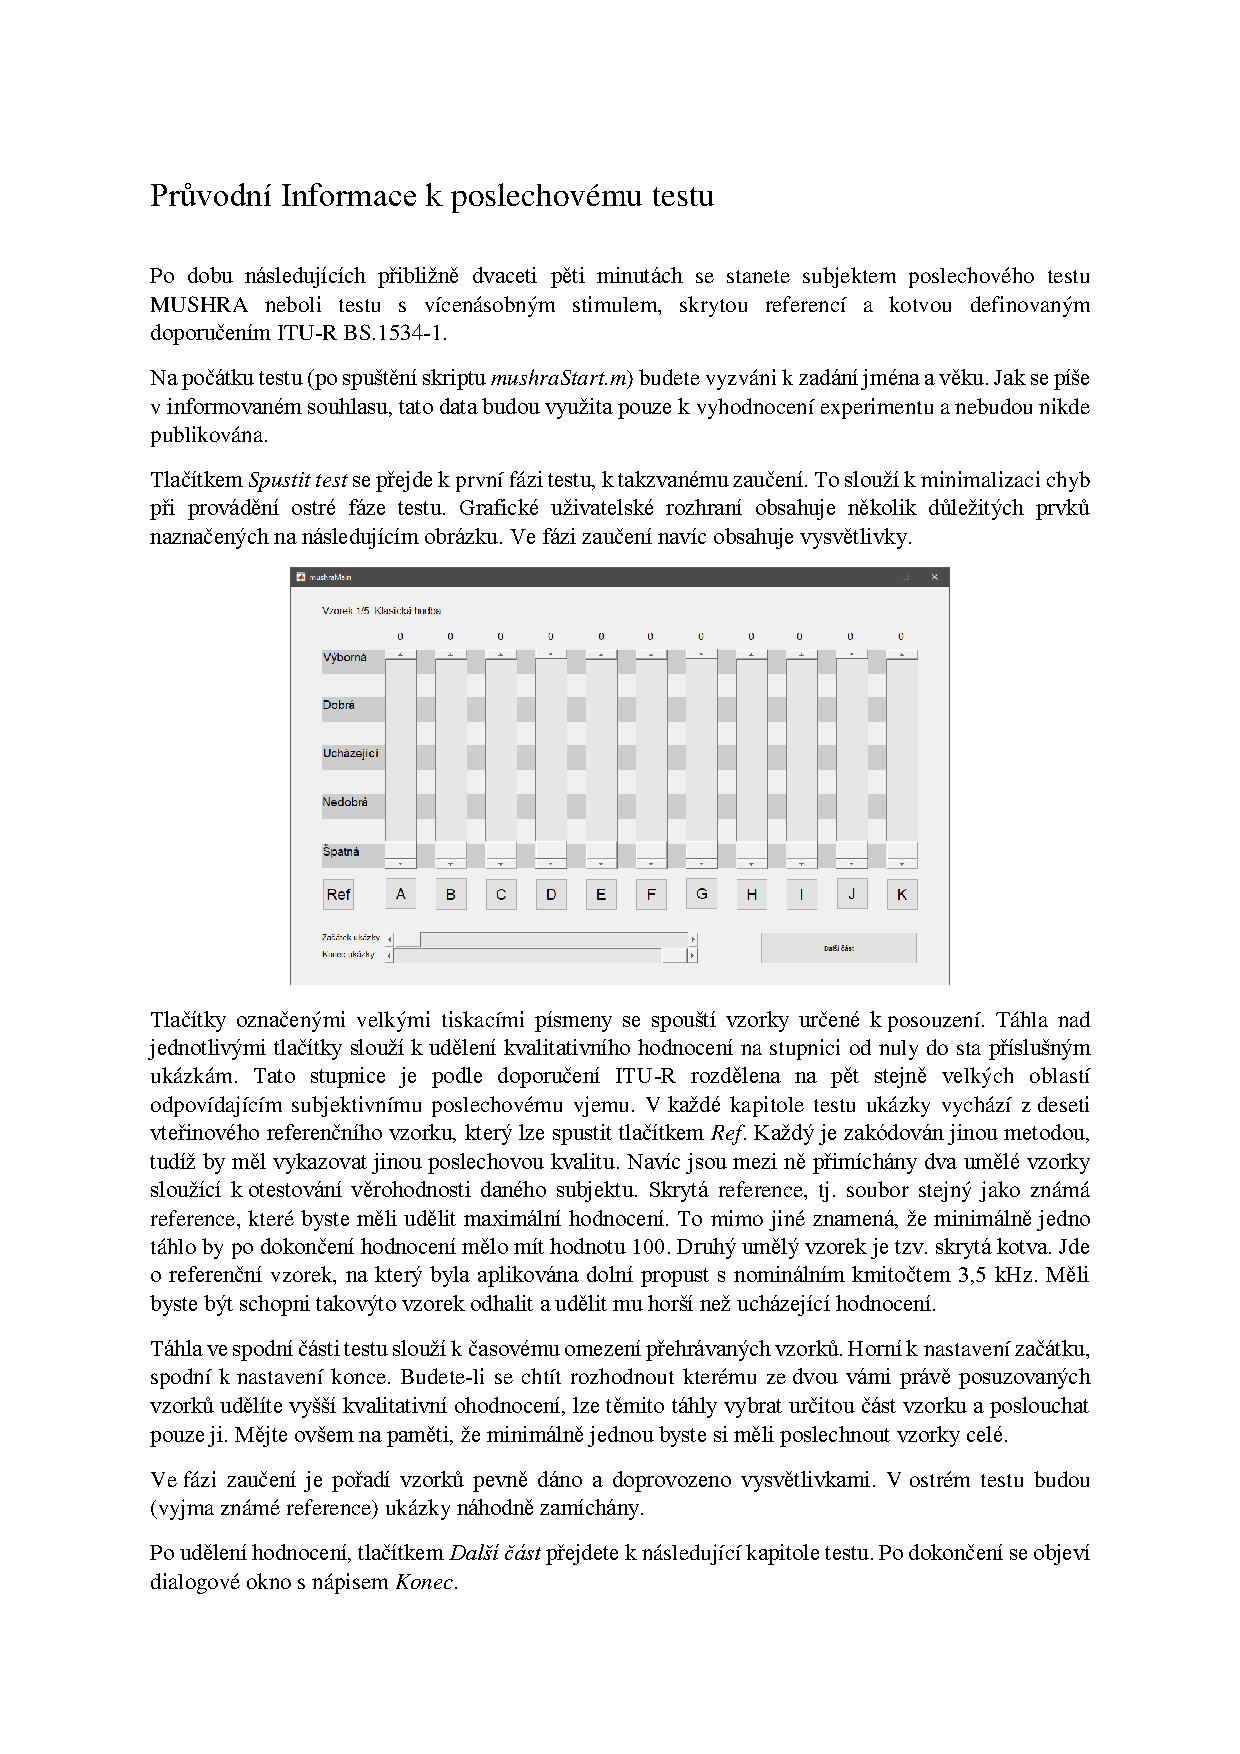
\includegraphics[page=1,width=.55\textwidth]{pdf/info.pdf}}
    \label{pdf:info}
\end{figure}
\chapter{Podrobné výsledky objektivního hodnocení}
\label{app:3}
%\section{PEAQ Basic}

Zde jsou uvedeny výsledky objektivního hodnocení ostatními algoritmy.

\begin{figure}[h]
    \centering
    \begin{subfigure}{.5\textwidth}
        \centering
        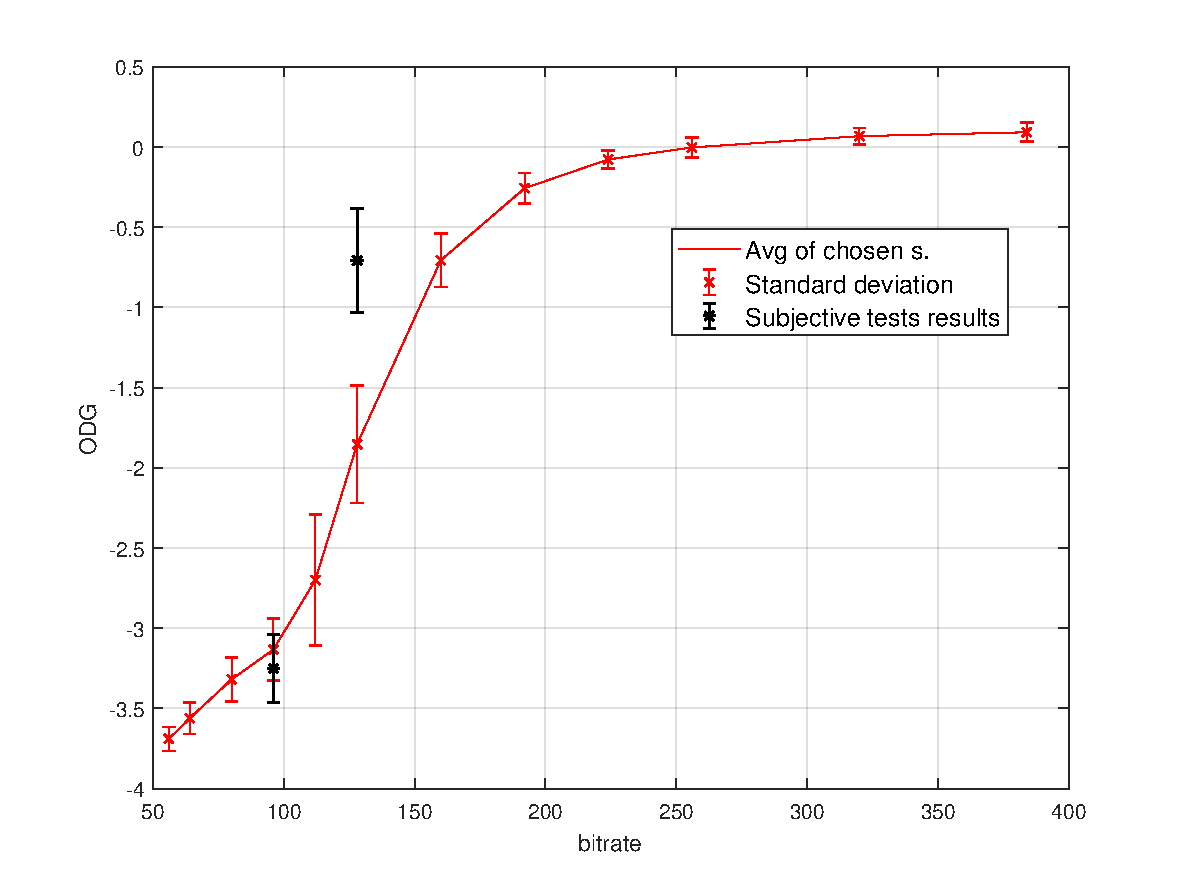
\includegraphics[width=1\linewidth]{pic/objective/mp2Basic.pdf}
        \caption{MP2}
        \label{app:bas:sub1}
    \end{subfigure}%
    \begin{subfigure}{.5\textwidth}
        \centering
        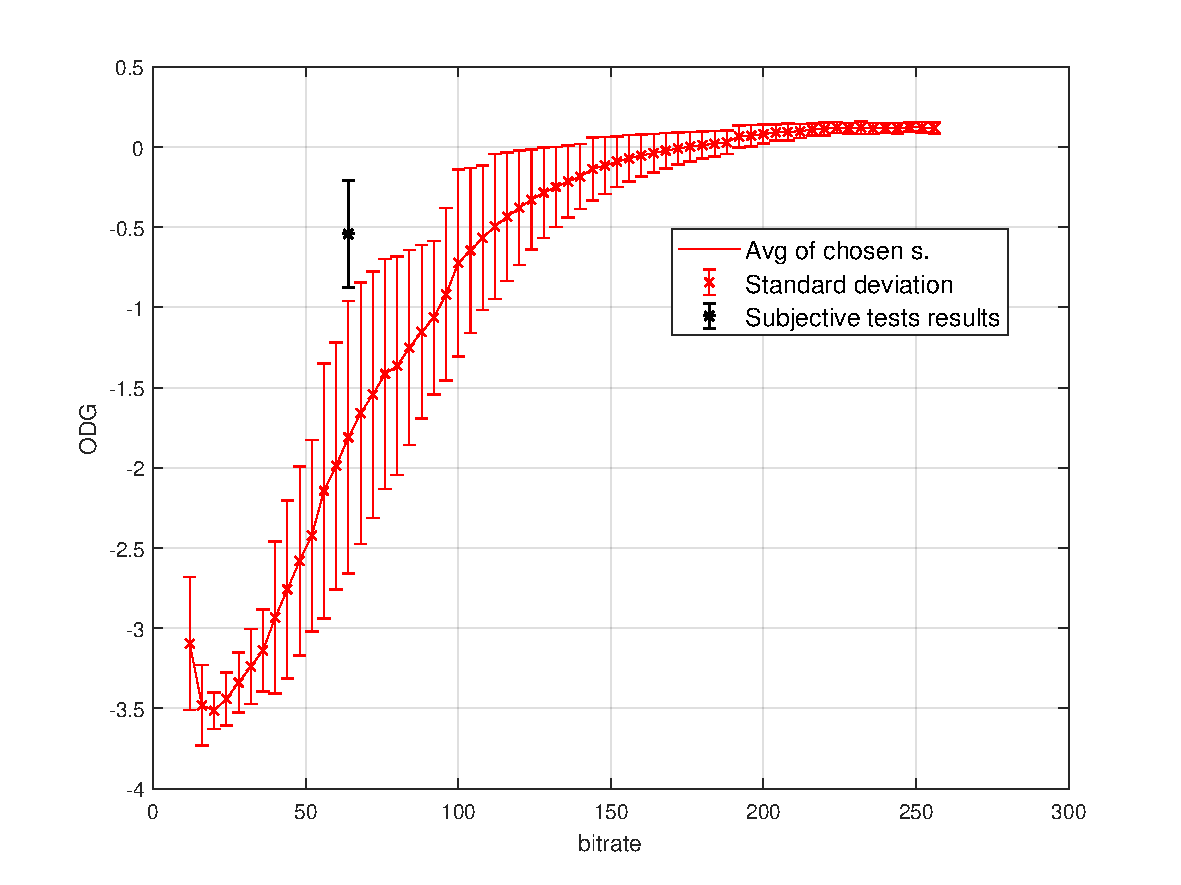
\includegraphics[width=1\linewidth]{pic/objective/lcBasic.pdf}
        \caption{LC-AAC}
        \label{app:bas:sub2}
    \end{subfigure}
\end{figure}
\begin{figure}[htb]\ContinuedFloat 
        \begin{subfigure}{.5\textwidth}
        \centering
        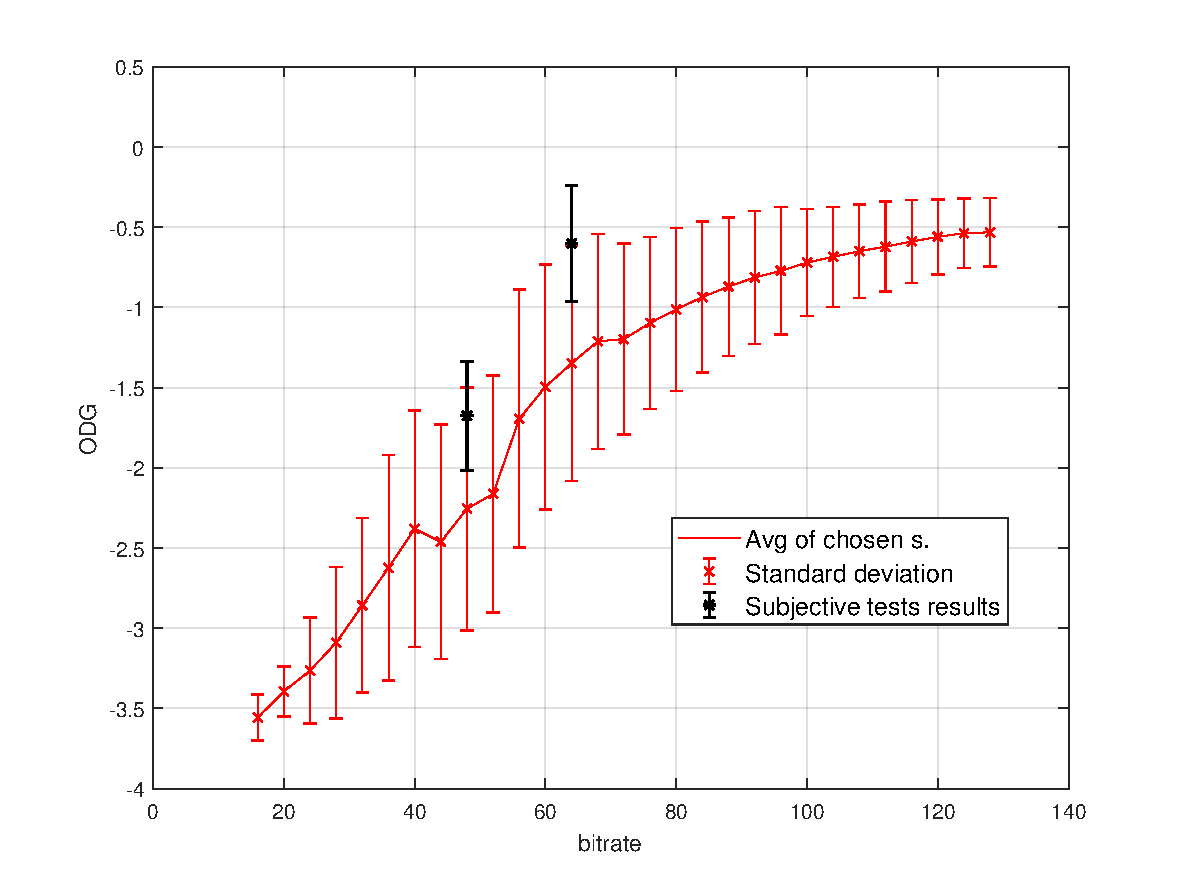
\includegraphics[width=1\linewidth]{pic/objective/heBasic.pdf}
        \caption{HE-AAC v1}
        \label{app:adv:sub3}
    \end{subfigure}%
        \begin{subfigure}{.5\textwidth}
        \centering
        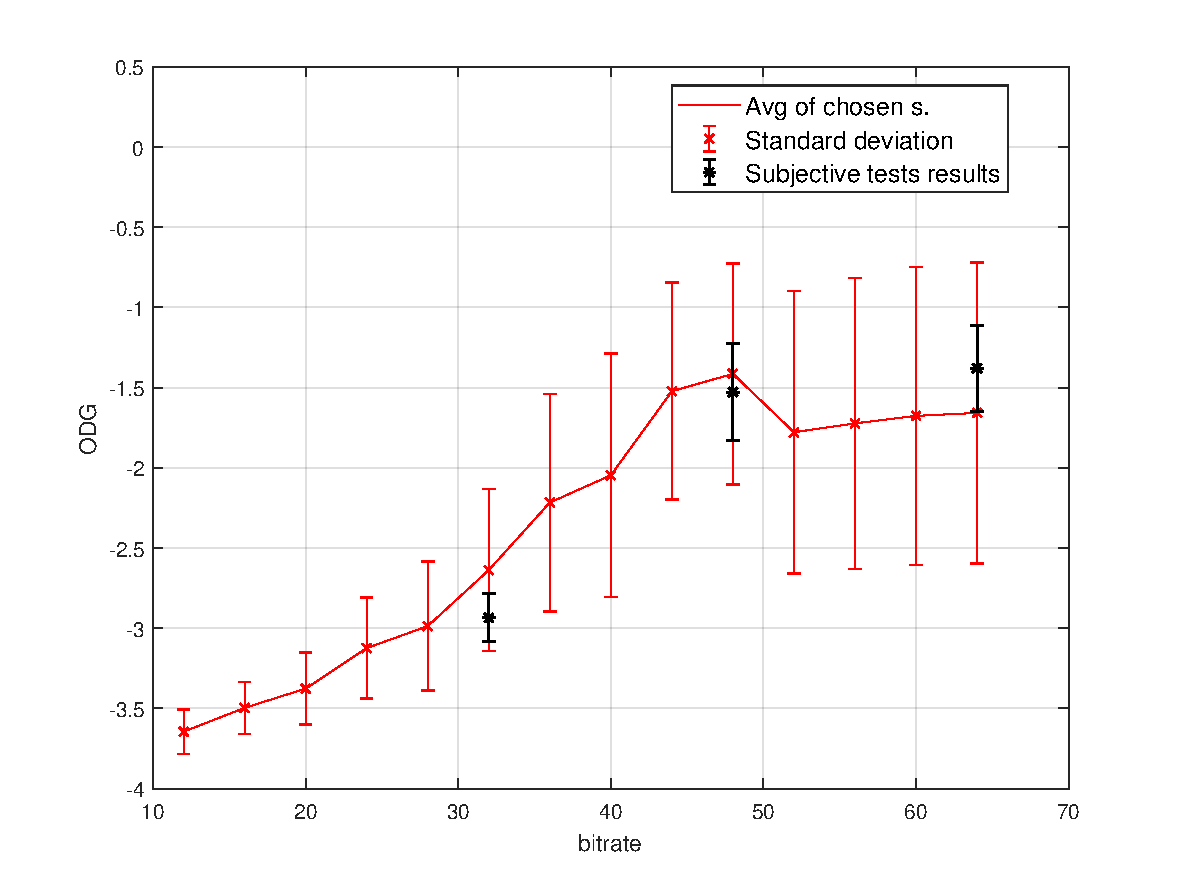
\includegraphics[width=1\linewidth]{pic/objective/hev2Basic.pdf}
        \caption{HE-AAC v2}
        \label{app:bas:sub4}
    \end{subfigure}%
    \\ 
        \begin{subfigure}{.5\textwidth}
        \centering
        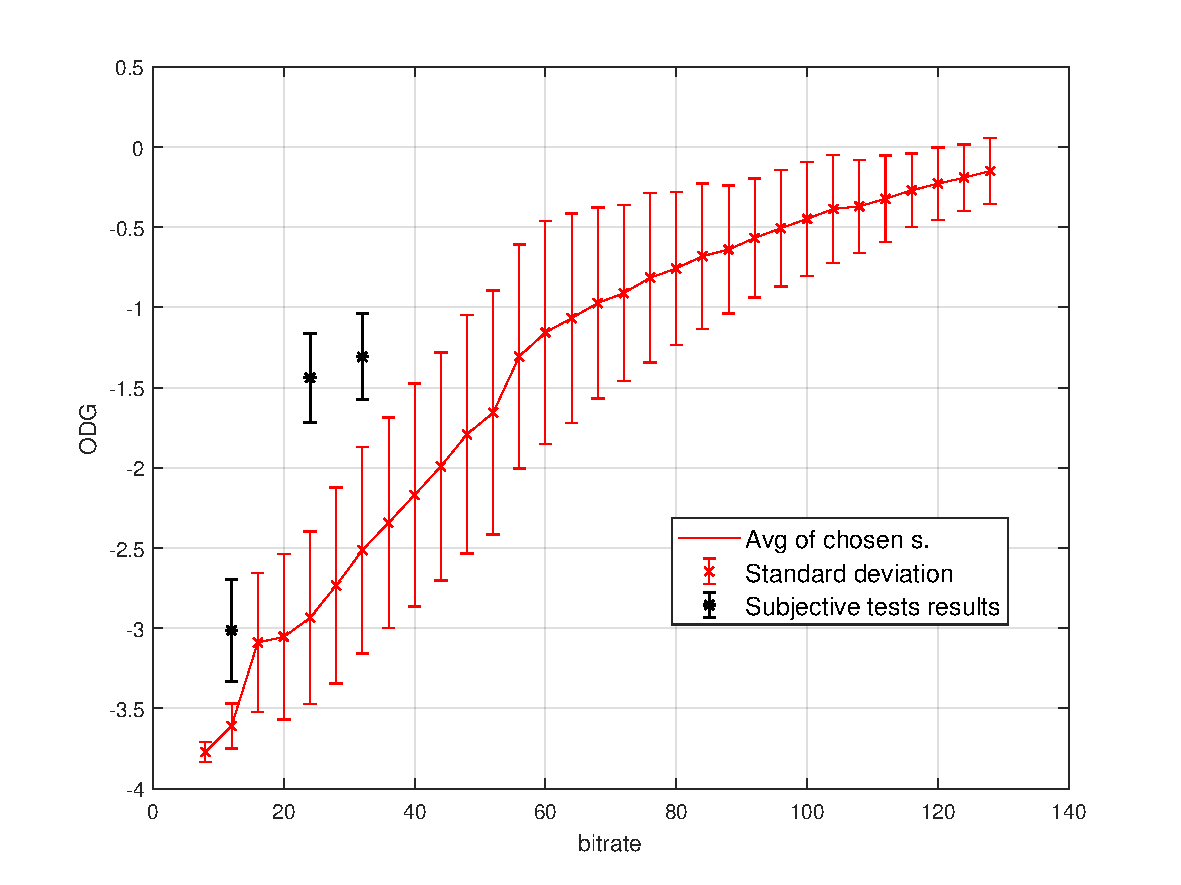
\includegraphics[width=1\linewidth]{pic/objective/opusBasic.pdf}
        \caption{Opus}
        \label{app:bas:sub5}
    \end{subfigure}%
        \begin{subfigure}{.5\textwidth}
        \centering
        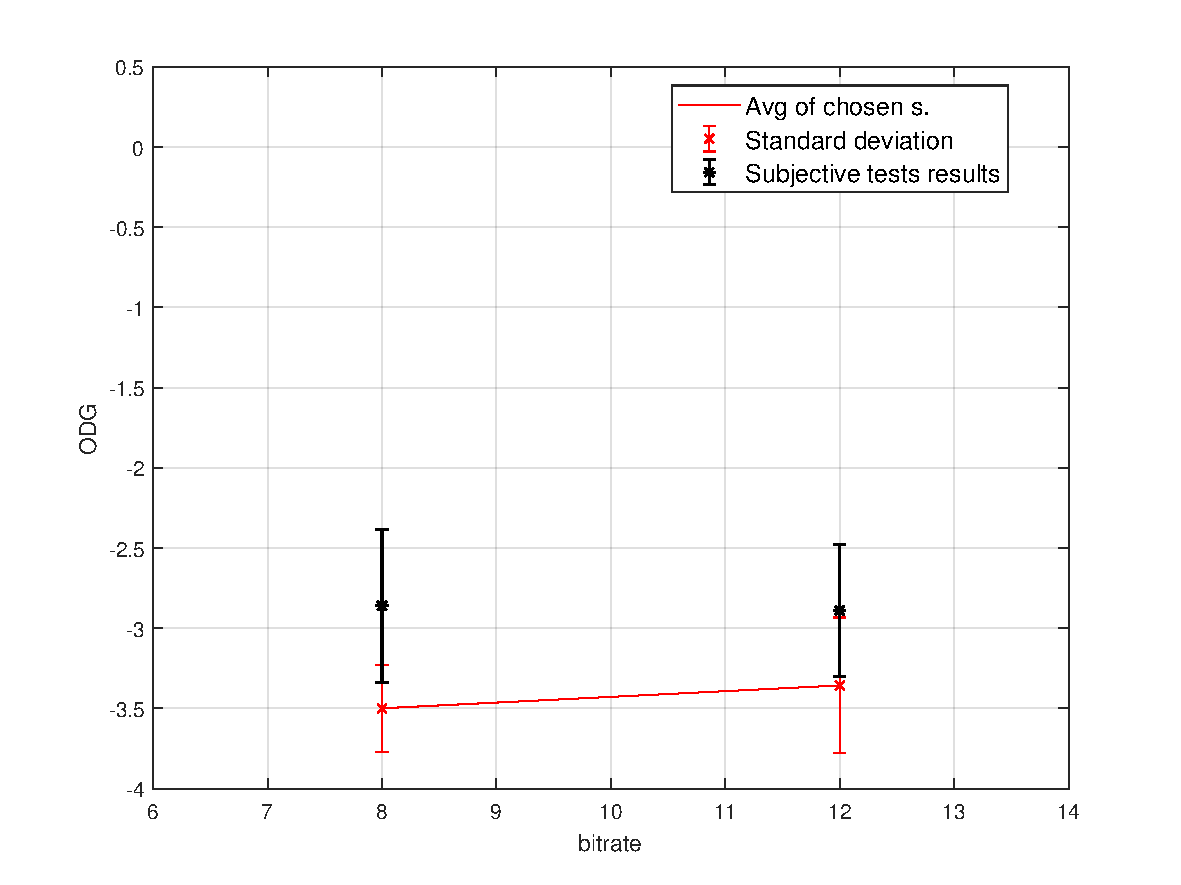
\includegraphics[width=1\linewidth]{pic/objective/xheBasic.pdf}
        \caption{xHE-AAC}
        \label{app:bas:sub6}
    \end{subfigure}%
    \caption{Hodnocení algoritmem PEAQ Basic.} 
\label{app:Basic}
\end{figure}

%\section{PEAQ Basic}

\begin{figure}[h]
    \centering
    \begin{subfigure}{.5\textwidth}
        \centering
        \includegraphics[width=1\linewidth]{pic/objective/mp2Advanced.pdf}
        \caption{MP2}
        \label{app:adv:sub1}
    \end{subfigure}%
    \begin{subfigure}{.5\textwidth}
        \centering
        \includegraphics[width=1\linewidth]{pic/objective/lcAdvanced.pdf}
        \caption{LC-AAC}
        \label{app:adv:sub2}
    \end{subfigure}
    \\
        \begin{subfigure}{.5\textwidth}
        \centering
        \includegraphics[width=1\linewidth]{pic/objective/heAdvanced.pdf}
        \caption{HE-AAC v1}
        \label{app:sub3}
    \end{subfigure}%
        \begin{subfigure}{.5\textwidth}
        \centering
        \includegraphics[width=1\linewidth]{pic/objective/hev2Advanced.pdf}
        \caption{HE-AAC v2}
        \label{app:adv:sub4}
    \end{subfigure}%
        \\
        \begin{subfigure}{.5\textwidth}
        \centering
        \includegraphics[width=1\linewidth]{pic/objective/opusAdvanced.pdf}
        \caption{Opus}
        \label{app:adv:sub5}
    \end{subfigure}%
        \begin{subfigure}{.5\textwidth}
        \centering
        \includegraphics[width=1\linewidth]{pic/objective/xheAdvanced.pdf}
        \caption{xHE-AAC}
        \label{app:adv:sub6}
    \end{subfigure}%
    \caption{Hodnocení algoritmem PEAQ Advanced} 
\label{app:Advanced}
\end{figure}


%\section{PEMO-Q}


\begin{figure}[h]
    \centering
    \begin{subfigure}{.5\textwidth}
        \centering
        \includegraphics[width=1\linewidth]{pic/objective/mp2Pemoq.pdf}
        \caption{MP2}
        \label{app:pem:sub1}
    \end{subfigure}%
    \begin{subfigure}{.5\textwidth}
        \centering
        \includegraphics[width=1\linewidth]{pic/objective/lcPemoq.pdf}
        \caption{LC-AAC}
        \label{app:pem:sub2}
    \end{subfigure}
    \\
        \begin{subfigure}{.5\textwidth}
        \centering
        \includegraphics[width=1\linewidth]{pic/objective/hePemoq.pdf}
        \caption{HE-AAC v1}
        \label{app:pem:sub3}
    \end{subfigure}%
        \begin{subfigure}{.5\textwidth}
        \centering
        \includegraphics[width=1\linewidth]{pic/objective/hev2Pemoq.pdf}
        \caption{HE-AAC v2}
        \label{app:pem:sub4}
    \end{subfigure}%
        \\
        \begin{subfigure}{.5\textwidth}
        \centering
        \includegraphics[width=1\linewidth]{pic/objective/opusPemoq.pdf}
        \caption{Opus}
        \label{app:pem:sub5}
    \end{subfigure}%
        \begin{subfigure}{.5\textwidth}
        \centering
        \includegraphics[width=1\linewidth]{pic/objective/xhePemoq.pdf}
        \caption{xHE-AAC}
        \label{app:pem:sub6}
    \end{subfigure}%
    \caption{Hodnocení algoritmem PEMO-Q.} 
\label{app:Pemoq}
\end{figure}




% % Add the index if it is requested above
% \ifx\printindex\undefined\relax\else\cleardoublepage\phantomsection\addcontentsline{toc}{chapter}{\protect\numberline{}{Index}}\fi
% \ifx\printindex\undefined\relax\else\printindex\fi
\end{document}
